\documentclass[oldfontcommands, b5paper]{memoir}%\stockbv\pageaiv

\usepackage[T1]{fontenc}
\usepackage[utf8]{inputenc}
\usepackage[a4paper]{geometry}%[b5paper]{geometry}%[a4paper]{geometry}
\geometry{verbose,tmargin=2.5cm,bmargin=2.5cm,lmargin=2.5cm,rmargin=2.5cm}
%\usepackage{geometry}
%\geometry{
% b5paper
% total={170mm,257mm},
% left=20mm,
% top=20mm,
% } 
\pagestyle{Ruled}
%\settypeblocksize{6.5in}{4.5in}{*}
%\setlrmargins{*}{*}{1}
%\checkandfixthelayout
\usepackage{array}
\usepackage{verbatim}
\usepackage{prettyref}
\usepackage{booktabs}
\usepackage{textcomp}
\usepackage{url}
\usepackage{amsmath}
\usepackage{chemarr}%flechas para reacciones químicas (SFER.tex)
\usepackage{graphicx}
\usepackage{amssymb}
\usepackage{nomencl}
\usepackage[usenames,dvipsnames]{xcolor}
%\usepackage{subfig}
\usepackage{subcaption}


\newcommand\blfootnote[1]{%
  \begingroup
  \renewcommand\thefootnote{}\footnote{#1}%
  \addtocounter{footnote}{-1}%
  \endgroup
}

%\includeonly{Discusion}

\OnehalfSpacing

% the following is useful when we have the old nomencl.sty package
% \providecommand{\printnomenclature}{\printglossary}
% \providecommand{\makenomenclature}{\makeglossary}
\makenomenclature

\usepackage[caption=false]{subfig}
%Configuración de los caption
%\PassOptionsToPackage{caption=false}{subfig}%Evita que el paquete subfig lo descabale todo
\captiontitlefont{\itshape}
\captionnamefont{\scshape}
\captionsetup{font=footnotesize}
% \captionstyle{\centering}
\hangcaption


%\usepackage[spanish]{babel}
%\addto\shorthandsspanish{\spanishdeactivate{~<>}}
 

\usepackage[emulate=units]{siunitx}
\sisetup{per=fraction, fraction=nice}
\newunit{\wattpeak}{Wp}
\newunit{\watthour}{Wh}
\newunit{\watt}{W}
\newunit{\metro}{m}

% \usepackage{lscape}
\usepackage{mathpazo}%Letra palatino con fuentes para matemáticas
\usepackage{flafter}%obliga a que los flotantes aparezcan después de su referencia
\usepackage{memhfixc}
\usepackage{mempatch}


\raggedbottom
\sloppybottom
\clubpenalty=10000
\widowpenalty=10000

%\raggedbottomsection
\feetbelowfloat

% !! esta seccion esta comentada en veleta

\usepackage[citestyle=alphabetic, bibstyle=alphabetic, maxbibnames=5, minbibnames=3, backend=bibtex, doi=true, url=true]{biblatex}

\DefineBibliographyStrings{spanish}{%
  andothers        = {et\addabbrvspace al\adddot},
  andmore          = {et\addabbrvspace al\adddot},
  in               = {},
}

% \addbibresource{../biblio.bib}
\addbibresource{Data.bib}

\let\cite\parencite

\renewcommand{\bibsection}{%
	\chapter*{\bibname}
	\bibmark
	\phantomsection
	\addcontentsline{toc}{chapter}{\bibname}
	\prebibhook}
\renewcommand{\bbltechreport}{Informe T\'ecnico}

% !!

%definition of some colors I could use.      
\definecolor{amaranth}{rgb}{0.9, 0.17, 0.31}
\definecolor{brightmaroon}{rgb}{0.76, 0.13, 0.28}

\usepackage{hyperref}


\hypersetup{
    bookmarks=true,         % show bookmarks bar?
    unicode=true,          % non-Latin characters in Acrobat’s bookmarks
    bookmarksnumbered=false,
    bookmarksopen=false,
    breaklinks=true,
    backref=true,
    pdftoolbar=true,        % show Acrobat’s toolbar?
    pdfmenubar=true,        % show Acrobat’s menu?
    pdffitwindow=false,     % window fit to page when opened
    pdfstartview={FitH},    % fits the width of the page to the window
    pdftitle={Tesis Claudia},    % title
    pdfauthor={Claudia Gutiérrez},     % author
    pdfsubject={Energia Solar Fotovoltaica},   % subject of the document
    pdfcreator={AucTeX/Emacs},   % creator of the document
    pdfproducer={LaTeX}, % producer of the document
    pdfkeywords={radiación solar, energía solar fotovoltaica, energías
    renovables}, % list of keywords
    pdfnewwindow=true,      % links in new window
    pdfborder={0 0 0},
    colorlinks=true,       % false: boxed links; true: colored links
    linkcolor=grey,          % color of internal links
    citecolor=brigthmaroon %BrickRed,        % color of links to bibliography
    filecolor=black,      % color of file links
    urlcolor=Blue           % color of external links 
}
	

\DeclareSIUnit\kWh{kWh}
\DeclareSIUnit\Wh{Wh}
\DeclareSIUnit\Wp{Wp}
\DeclareSIUnit\kWp{kWp}
\DeclareSIUnit\amperehour{Ah}
\DeclareSIUnit\celula{celula}

%\spanishdecimal{.} %Para que no lo sustituya automáticamente por comas
\addto\captionsspanish{%
\def\tablename{Tabla}%
\def\listtablename{\'Indice de tablas}}

\renewcommand\nomname{Nomenclatura}
\def\nompreamble{\addcontentsline{toc}{chapter}{\nomname}\markboth{\nomname}{\nomname}}


%\@addtoreset{equation}{section}
%\renewcommand{\theequation}{\thesection.\arabic{equation}}
%\numberwithin{equation}{section}
%\@addtoreset{table}{section}
%\renewcommand{\thetable}{\thesection.\arabic{table}}
%\numberwithin{table}{section}
%\@addtoreset{figure}{section}
%\renewcommand{\thefigure}{\thesection.\arabic{figure}}
%\numberwithin{figure}{section}


%\declarebtxcommands{spanish}{%
 % \def\btxphdthesis#1{\protect\foreignlanguage{spanish}{Tesis Doctoral}}%
%}
%\setbibliographyfont{lastname}{\scshape}%Pone los autores en Small Caps



%Configuración de MEMOIR
%%Pone la fecha en SMALL CAPS y hacia la derecha
%%pagina 60 de memman.pdf
\pretitle{\vfill \begin{center} \bfseries\HUGE \color{Black}}% \scshape \HUGE \color{Black}}
\posttitle{\par\end{flushright}}

\preauthor{\begin{center} \large}% \scshape}
\postauthor{\par\end{flushright}}

\date{}
\predate{\vfill \begin{flushright}\large\scshape}
\postdate{\par\end{flushright}\vfill}

\setsecnumdepth{subsection}


%\definecolor{ared}{rgb}{.647,.129,.149}
%\renewcommand{\colorchapnum}{\color{ared}}
%\renewcommand{\colorchaptitle}{\color{ared}}
%\chapterstyle{pedersen}
\chapterstyle{ger}

\setlength{\afterchapskip}{35pt}
\maxtocdepth{section}

% \setcounter{topnumber}{3}
%\setcounter{bottomnumber}{2}
%\setcounter{totalnumber}{4}
\renewcommand{\topfraction}{0.85}
\renewcommand{\bottomfraction}{0.5}
\renewcommand{\textfraction}{0.15}
\renewcommand{\floatpagefraction}{0.7}


%Centra las figuras en los flotantes y los enmarca
\makeatletter
\renewenvironment{figure}[1][]{%
     	\@float{figure}%
		%\begin{framed}    
		\precaption{\rule{\linewidth}{0.4pt}\par}%En las figuras el caption va debajo
		%\hrule\vspace{\onelineskip}
		\centering
		  }{%
		%\end{framed}
		%\postcaption{\rule{\linewidth}{0.4pt}}
		%\vspace{\onelineskip}\hrule
    	\end@float	
}
\makeatother

\makeatletter
\renewenvironment{table}[1][]{%
      	\@float{table}%
		%\begin{framed}    
		\postcaption{\rule{\linewidth}{0.4pt}\par}%En las tablas el caption va encima
		\centering
		  }{%
		%\end{framed}
    	\end@float	
}
\makeatother


\renewcommand{\textfloatsep}{10pt}%Espacio entre el flotante y el texto

%backgroung image
\usepackage{eso-pic} 

%http://stackoverflow.com/questions/240097/how-to-create-a-background-image-on-titlepage-with-latex
\newcommand\BackgroundPic{
  \put(350,-150){
    \parbox[b][0.5\paperheight]{0.5\paperwidth}{%
      \includegraphics[scale=0.5]{../figs/johnny_automatic_old_sun}%
}}}

\newcommand\BackgroundPicLight{
  \put(350,-150){
    \parbox[b][0.5\paperheight]{0.5\paperwidth}{%
 %     \vfill 
%\centering
      \includegraphics[scale=0.5]{../figs/johnny_automatic_old_sun_light}%
%\vfill
}}}

%claudia

\renewenvironment{abstract}%
{\clearpage\null \vfill\begin{center}%
\bfseries\abstractname\end{center}}%
{\vfill\null}

%%%% claudia:
% \usepackage{color,calc,graphicx,soul,fourier}
% \definecolor{nicered}{rgb}{.647,.129,.149}
% \makeatletter
% \newlength\dlf@normtxtw
% \setlength\dlf@normtxtw{\textwidth}
% \def\myhelvetfont{\def\sfdefault{mdput}}
% \newsavebox{\feline@chapter}
% \newcommand\feline@chapter@marker[1][4cm]{%
% \sbox\feline@chapter{%
% \resizebox{!}{#1}{\fboxsep=1pt%
% \colorbox{nicered}{\color{white}\bfseries\sffamily\thechapter}%
% }}%
% \rotatebox{90}{%
% \resizebox{%
% \heightof{\usebox{\feline@chapter}}+\depthof{\usebox{\feline@chapter}}}%
% {!}{\scshape\so\@chapapp}}\quad%
% \raisebox{\depthof{\usebox{\feline@chapter}}}{\usebox{\feline@chapter}}%
% }
% \newcommand\feline@chm[1][4cm]{%
% \sbox\feline@chapter{\feline@chapter@marker[#1]}%
% \makebox[0pt][l]{% aka \rlap
% \makebox[1cm][r]{\usebox\feline@chapter}%
% }}
% \makechapterstyle{daleif1}{
% \renewcommand\chapnamefont{\normalfont\Large\scshape\raggedleft\so}
% \renewcommand\chaptitlefont{\normalfont\huge\bfseries\scshape\color{nicered}}
% \renewcommand\chapternamenum{}
% \renewcommand\printchaptername{}
% \renewcommand\printchapternum{\null\hfill\feline@chm[2.5cm]\par}
% \renewcommand\afterchapternum{\par\vskip\midchapskip}
% \renewcommand\printchaptertitle[1]{\chaptitlefont\raggedleft ##1\par}
% }
% \makeatother
% \chapterstyle{daleif1}
%probar bluebox

% \usepackage{calc,color}
% \newif\ifNoChapNumber
% \newcommand\Vlines{%
% \def\VL{\rule[-2cm]{1pt}{5cm}\hspace{1mm}\relax}
% \VL\VL\VL\VL\VL\VL\VL}
% \makeatletter
% \setlength\midchapskip{0pt}
% \makechapterstyle{VZ43}{
% \renewcommand\chapternamenum{}
% \renewcommand\printchaptername{}
% \renewcommand\printchapternum{}
% \renewcommand\chapnumfont{\Huge\bfseries\centering}
% \renewcommand\chaptitlefont{\Huge\bfseries\raggedright}
% \renewcommand\printchaptertitle[1]{%
% \Vlines\hspace*{-2em}%
% \begin{tabular}{@{}p{1cm} p{\textwidth-3cm}}%
% \ifNoChapNumber\relax\else%
% \colorbox{black}{\color{white}%
% \makebox[.8cm]{\chapnumfont\strut \thechapter}}
% \fi
% & \chaptitlefont ##1
% \end{tabular}
% \NoChapNumberfalse
% }
% \renewcommand\printchapternonum{\NoChapNumbertrue}
% }
% \makeatother
% \chapterstyle{VZ43}

\usepackage{fourier} % or what ever
\usepackage[scaled=0.92]{helvet}%. Sans serif - Helvetica
\usepackage{color,calc}
\newsavebox{\ChpNumBox}
\definecolor{ChapBlue}{rgb}{0.00,0.65,0.65}
\makeatletter
\newcommand*{\thickhrulefill}{%
\leavevmode\leaders\hrule height 1\p@ \hfill \kern \z@}
\newcommand*\BuildChpNum[2]{%
\begin{tabular}[t]{@{}c@{}}
\makebox[0pt][c]{#1\strut} \\[.5ex]
\colorbox{ChapBlue}{%
\rule[-10em]{0pt}{0pt}%
\rule{1ex}{0pt}\color{black}#2\strut
\rule{1ex}{0pt}}%
\end{tabular}}
\makechapterstyle{BlueBox}{%
\renewcommand{\chapnamefont}{\large\scshape}
\renewcommand{\chapnumfont}{\Huge\bfseries}
\renewcommand{\chaptitlefont}{\raggedright\Huge\bfseries}
\setlength{\beforechapskip}{20pt}
\setlength{\midchapskip}{26pt}
\setlength{\afterchapskip}{40pt}
\renewcommand{\printchaptername}{}
\renewcommand{\chapternamenum}{}
\renewcommand{\printchapternum}{%
\sbox{\ChpNumBox}{%
\BuildChpNum{\chapnamefont\@chapapp}%
{\chapnumfont\thechapter}}}
\renewcommand{\printchapternonum}{%
\sbox{\ChpNumBox}{%
\BuildChpNum{\chapnamefont\vphantom{\@chapapp}}%
{\chapnumfont\hphantom{\thechapter}}}}
\renewcommand{\afterchapternum}{}
\renewcommand{\printchaptertitle}[1]{%
\usebox{\ChpNumBox}\hfill
\parbox[t]{\hsize-\wd\ChpNumBox-1em}{%
\vspace{\midchapskip}%
\thickhrulefill\par
\chaptitlefont ##1\par}}%
}
\chapterstyle{BlueBox}

\epigraphfontsize{\small\itshape}
\setlength\epigraphwidth{8cm}
\setlength\epigraphrule{0pt}
  
% \renewcommand{\prebibhook}{Nota: todos los enlaces URL han sido
%   comprobados en Marzo de 2013.}

\begin{document}

%\AddToShipoutPicture*{\BackgroundPic}


%\pagestyle{empty}
\begin{titlingpage}


\title{Características espacio-temporales de la producción fotovoltaica en el área Euro-Mediterránea: análisis climático}

\author{Claudia Gutiérrez Escribano}
\date{}

\maketitle


\end{titlingpage}

\frontmatter

%\AddToShipoutPicture{\BackgroundPicLight}

%\include{Licencia}

\chapter{Preface}
Applied science has made societies evolved trough the linked between the basic science and the 'ingenios' that implement the structural knowdlege to the individual dailylife. The bridge between the fundamental studies and its evolution or transformation into something applied (useful) for the societies development is been a matter of interpretation or 'translation' (so interpreters/translator) that have been able to find the accurate language to exchange this knowdlege.

% Esta transversalidad entre las disciplinas básicas de la física, la química o la biología con distintas acepciones prácticas, la mayoría de ellas recogidas bajo el paraguas de las ingenierías, desemboca ineludiblemente en una transformación de lo abstracto en lo tangible con la premisa o el ideal de mejorar el bienestar de las sociedades presentes y futuras.

Transversality between the fundamental disciplines of physiscs, chemistry or biology and their different applied branches, most of them under the umbrella of ingenieering, end unavoidably into a transformation from the abstract
ion to the tanglible with the premise or ideal of improving wellbeing of present and future societies.

% Es sin embargo muy probable, que esta concepción de la aplicación científica haya desembocado en el mayor problema al que la humanidad tiene que hacer frente desde su existencia, el cambio climático. Siendo este antropocentrismo parte del problema, y no de la solución. Jorge Wasenberg escibe en su libro, ``el pensador intruso'' en referencia a la evolución de la ciencia y el progreso subyacente lo siguiente:

However, it is very likely that this conception of the scientific application had lead to the most challeging problem that humanity has to face from its existance, climate change, being this anthropocentrism part of the problem and not of the solution.

In his book ``El pensador intruso'', Jorge Wasengber wrote about the evolution of science and the underlying progress what follows: 

'There are above all two vices that tend to set 'pre-cooked' ideollogy into science. First is base on different kinds of anthropocentrism and consist in put the knowdlege subjet into the cosmos's center. The history of knowdlege is the witness: each time we 'barremos' the 'I' from the spot, the knowdlege progresses and only because of it.'
% ``Existen sobre todo dos vicios que tienden a inyectar ideología precocinada en la ciencia. Una de ellas se basa en las distintas formas de antropocentrismo y consiste en situar instintivamente al sujeto del conocimiento en el centro del cosmos. La historia del conocimiento es testigo: cada vez que barremos el Yo del centro del escenario el conocimiento avanza, y avanza sólo por ello.''

% Sin caer en lo pretencioso, este trabajo contribuye a la imbricación entre la ciencia del cambio climático y la tecnología renovable de producción eléctrica con mayor potencial a día de hoy, la solar fotovoltaica.

\clearpage
%\include{Creditos}
\tableofcontents
%\clearpage
%\listoffigures*
%\clearpage
%\listoftables*

%\printnomenclature{}

\cleardoublepage{}

\begin{abstract}
Resumen de la tesis
\end{abstract}

%\abstractname

\mainmatter

% Este documento contiene el índice del manuscrito de la tesis.
%\documentclass[12pt,a4paper]{report}
%\usepackage{graphicx}
 
%\title{Introduction}
%\author{Claudia Guti\'errez}
%\date{ January 2018}


%\begin{document}

%\maketitle

%\tableofcontents{}

%%%%%%%%%%%%%%%%%%%%%%%%%%%%%%%%%%%%%%%%%%%%%%%%%%%%%%%%%%%%%%%%%%%%%%%%%%%%%%%%%%%%%%
\part{Introduction\label{cha:intro}}

\chapter{Context and introduction\label{context}}

\epigraphfontsize{\small\itshape}
\epigraph{''Begin at the beginning,'' the King said gravely, ''and go on till you
come to the end: then stop.''}{--- \textup{Lewis Carroll}, Alice in Wonderland}

\section{A changing world} 

% Ideas a desarrollar:

% * Un mundo en constante evolución.
% * Cambio climático
% * Transición energética global
% * Cambios sociales/políticos.
% * Migraciones

It is said that nothing is permanent except for change. We are in a constantly evolving world where, unavoidably, some of these changes will go over us without us  being able to adapt to them. Meanwhile, other changes will go unnoticed because of their slowness or because they are not part of our main concerns. It seems paradox to think that some of those human induced changes, consciously or unconsciously, willingly or by mistake, will make human beings resist an get adapted as a species against the consequences of something that they themselves created. 

The evolution and development of nations has been linked since the first Industrial Revolution to an increment on the energy demand. The use of fossil fuels since the vapour engine has changed the well-being of societies. Related to this increase, the green house gasses (GHG) emissions and their concentration in the atmosphere has risen dramatically in contrast to pre-Industrial times. Global warming, with its origin in human activities, is one of the biggest challenges of adaptation for human beings. The \textit{anisotropic} character of the associated impacts of climate change puts our solidarity with the most vulnerable and less responsible communities on trial.

Some people believe we are in what has been described as the Third Industrial Revolution \cite*{Rifkin2012}, a process of exponential scientific-technological development, characterised as a convergence of the evolution of renewable energy technologies and the massive use of new communication technologies. The ongoing energy transition should be the answer to committed citizens that find those technologies as an alternative and an answer to the environmental challenges and associated consequences.     

The actual context is characterised by an advanced globalisation where the borders have been blurred through telecommunications development and international migration movements are becoming more feasible. In 2015, there were 100 millions more people living in a different country of its birth country than in 1990 [International Organisation for Migration]. Most of that movements are related to work opportunities or family issues. However, the increase of the population and the rising demand of natural resources to support a system based on the continuous growth lead to geopolitic conflicts and the depletion of natural resources \cite*{Rosa2012,commoner1991}, what supposes an increase in migration movements of different character. Populations migrate away from conflict areas or most affected areas by natural disasters [ref ``Environmental Migration Portal'', ref ``International Organisation for Migration'']. In that sense, these movements affect most vulnerable people and require special attention.

In order to address the human needs in a juncture of population growth, increase of energy demand and environmental crisis, a paradigm shift is needed. This change would mean recognising our interdependence with every ecosystem and all living beings as well as recognising the importance of nature itself. In 1962, Thomas Kuhn wrote in his book  "The Structure of Scientific Revolutions" that a paradigm shift does not occur until the adherents of the old paradigm are replaced with the new generation. We should then wait to see the end of this paradigm shift hoping that it is not too late.

\section{Renewable Energy}

%\subsection{Concept of energy}

% The physics concept of \textbf{energy} is defined as the capacity of a system to perform a work and it is divided into two groups: kinetic energy, that is related to the movement of the system, and the potential energy, related to its position. For this fundamental classification, mechanical energy, electromagnetic and thermal energy are encompassed in the kinetic energy group, while the chemical energy or the gravitational potential energy, as it is the case of hydropower,  are inside the potential energy group.
 
% \subsection{Types and classification}

% It is elementary to delimit the differences between kinds and sources of energy. Sources of energy are defined as those from which useful energy can be extracted, and directly applied to its purpose (being this one movement, electricity production or metabolic processes) or by undergoing any transformation process.

In the context of society's energy consumption we call \textbf{primary energy sources} those from whom, after a process of extraction or transformation and transport, we are able to obtain final energy to be used. Regarding that, we consider fossil fuels as a primary energy source, as well as hydro-power, solar energy or biomass. %These sources of primary energy provide the final energy that many times will be in the form of electricity. 

These primary energy sources can be classified depending on their origin, being \textbf{renewable} those ones that are inexhaustible. The sun, despite of its unquestionable finitude is considered inexhaustible as well, because of the difference in the temporal scale of  human existence and the life of such star, which is lots of magnitude orders above.

\subsection{History and evolution}

The use of renewable energy has come along the development of humanity since ancient times. From the use of biomass to get thermal energy to the transformation of wind energy into mechanical energy to be used in the traditional windmills or for shipping. It was around the middle of the 19Th century with the invention of the vapour engine that fossil fuels started to be used massively and linked to that, what was called the \textit{First Industrial Revolution}. This period meant a big technological development that directly impacted positively on the societies's  wellbeing, at least to those from the richest or western countries.

This economic development brought about an increase on the fossil fuels demand that grew up exponentially during the 20Th century. Societies were more and more dependent on energy and evolved turning a blind eye to the reality that the base of their development are finite resources unequally distributed around the globe.

The first step to diversify sources of primary energy did not take place until the 70's, with the first petroleum crisis in 1973 (and the second crisis in 1979) \cite*{Sorensen1991}. The embargo of the petroleum producer countries had some important economic consequences on the importer ones, resulting in the fact that some of them started to consider new sources of energy in order to ensure stability and supply.

In the last decades, in addition to the socio-economic and geopolitic factors that have led to the need of limiting petroleum dependence from importer countries, the stimulus for the big increase of these alternative technologies, has come about due to their decreasing costs, which have the origin in the promotion of support policies. These policies have been driven by different organisms and governments that have created a virtuous cycle around these technologies. The decrease in costs thanks to the support and long-term view policies favours, at the same time, more national target commitments in the use of renewable energy to reduce GHG emissions and to fight against Climate Change. In 2017 more than 170 countries had established goals of renewable generation (IRENA2017).
 
In the actual context, the global energy demand is growing based on the needs of developing countries. It has been estimated that for 2040 it will be up by more than a quarter and it will have an associated shift from Europe to Asia, which will account for 40$\%$ of the energy demand (leaded by China) by that time [WEO2018].

Energy systems accounts for approximately 3/5 of all anthropogenic green house gas emissions [ref] which force us to find the way for a sustainable development that is able to afford human needs. This, unavoidably needs a decarbonization scenario for next years.  

In 2018 renewable energies account for the 18.2$\%$ of the \textbf{final energy consumption} according to the REN21 report [ref], with a share of 27$\%$ in heat generation and $25\%$ for electricity generation. Transport remains the sector with less share of renewable energies with only a $3\%$. These numbers, reflect that contribution of RE to the mix is continuosly growing, with increasing relevance in the electricity sector.

Future scenarios continue to project an increase in the energy demand with an overall decrease of the fossil fuel's share. At the same time, it is expected that the power sector increase its share in the final energy consumption distribution. According to that, renewable energies and specially solar and wind are key for delivering low carbon electricity [WEMC].

In 2017, the renewable capacity added was about 178 GW, accounting for the first time for more than 2/3 of global net electricity capacity growth and it was the PV the one that expanded the most with 97 GW [IEA].

%It has been reported that the integration of big shares of variable renewable energies, VRE, in the electricity system is not technically challenging as it was supposed. In many countries, 30$\%$ of VRE has been integrated into the system without a big increase in the storage [IRENA]. 

% \begin{itemize}
% \item Algunas estadísticas más sobre renovables  
% \item Remarcar el crecimiento de la fotovoltaica
% \item Terminar con: los escenarios futuros estarán determinados principalmente por 3 factores: un aumento en la demanda dada sobre todo por los países en desarrollo, una mayor electrificación y un descenso en el consumo de los combustibles fósiles.  
% \end{itemize}

 
\section{Photovoltaic Energy}

Among all the renewable energy technologies that had started to increase their installed capacity over the world, the photovoltaic energy is the one with higher ratios of installation in recent years and bigger rates of decreasing prices (80$\%$ since 2008 IRENA). Based on the completed projects in 2010, the levelized cost of energy, LCOE of PV projects fell 73$\%$ between 2010-2017 [REN21].

It has been mentioned that in 2017, RE had its largest anual increase of generation capacity [REN21], 178 GW, of RE from whom 55$\%$ correspond to PV technology. It means that it was added more capacity from solar PV than for any other technology. Nowadays, the total amount of solar PV capacity reach the 402 GW.

It is also forecasted that the PV capacity can grow by 600 GW more, which is more than the projected increase for any other technology combined. Within this framework, China would lead the PV installations, as it has happened for the 2017 when from the 97 GW of added PV capacity more than a half were installed there [REN21]. 

% Photovoltaic energy is based in the conversion of incident solar energy into electricity. This process is made by the photovoltaic systems whose basic unit that transform solar radiation intro electricity is the \textbf{solar cell.}

% \subsection{P-N junction}


% The fundamental physics of a solar cell is based in the \textbf{P-N junction}: a device that put in contact an extrinsic semiconductor, also called doped semiconductor, of type P and N.

% A N-type semiconductor is the one that has been doped with impurities: impurities are atoms with a higher number of valence electrons that the original semiconductor. Due to that, there is an excess of electrons, or negative charge carriers, in a cristal N-type. Once the new atom is icluded in the net, the extra-electrons goes to the conduction band of the semiconductor, reaining the associated positive charge in the net. This positive charge is called ``hole''. In a N-type semiconductor the concentration of electrons is bigger than the concentration of holes, what makes them the majority charge carrier. 

% In a P-type semiconductor the doping process consists in the addition to the net of some atoms with an smaller number of electrons than the original semiconductor. The holes density is then higher than the density of electrons.

% The P-N juntion put in contact the two semiconductors \ref{fig:pn}, which oringinates an imbalance due to the difference in concentration of charge carriers. That difference in the density starts a difsusion process from one side to another of the union, consisting in a movement of holes to the 'n' side through the valence band and a movement of the carriers of type 'p' to the opposite side (throught the conduction band). If carriers were not electrically charged, the diffusion process would continue until equilibrium. Due to their electrical charge, the ions linked to the net generates an electric field that oposse to the carriers diffusion. Then, it reaches the balance when the processes of diffusion and are equal.

% \begin{figure}[h!]
% \centering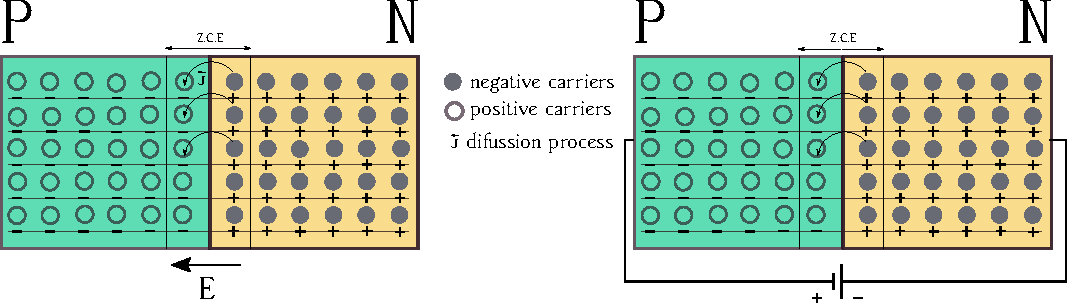
\includegraphics[width=0.6\textwidth]{figs/unionpn.pdf}
% \caption{PN junction, b) PN forward bias}
% \label{fig:pn}
% \end{figure}


% When the equilibrium is reached, the closer region to the interface called \textbf{space charge region}, the minority carriers are recombined and there are only electrically charged ions linked to the net. The electric field created by the ions generates a potential difference called, thermodinamical potential, that avoid the mjoroty carriers to cross to the other side f the juntion.

% \subsection{P-N forward bias}

% If we want to make a current to cross the P-N junction it is necessary to break the balance and that means that you need to reduce the thermodinamical potential. In order to do that, we can apply a potential difference between the edges of each semicunductor. If the P side has a positive voltage with respect to the N side, the PN junction is forward bias and reverse in the other case. In the forward biases the potential barrier is reduced and then electric charge cannot compensate the diffusion. The carriers of each side can go through the charge area and reach the other side, where they are minority carriers. At this moment the diffusion process creates two currents with two opposite directions, so they do not compensate each other and it generates an usable current. 

% If the P-N junction is reverse biases, which means that the P side has a negative voltage, the potential barrier increases and there will not be an usable current.

% Los procesos de generación de corriente en la unión P-N pueden resumirse en la ecuación de Shockley \ref{eq:shockley} que define la corriente generada por un diodo. El diodo es el dispositivo electrónico que se basa en el funcionamiento teórico de la unión P-N. En \ref{eq:shockley} $I_0$ es la corriente de saturación del diodo en oscuridad, $V$ la tensión aplicada y $m$ un factor para ajustar al funcionamiento real y $V_T$ el potencial térmico.

% The processes of current generation in the P-N junction can be summarized in the Shockley equation \ref{eq:shockley} that defines the current generated in a diode, an electronic deviced based in the P-N functioning. In \ref{eq:shockley} $I_0$  is the saturation current, $V$ the voltage applied and $m$ is a factor to adjust to real behaviour and $V_T$ is the thermodinamical potential.


% \begin{equation}
%   I_{D}=I_0\cdot [e^{{V}\over {m\cdot {V_{T}}}}-1]
% \label{eq:shockley}
% \end{equation}

% \subsection{Solar Cell}

% When the P-N junction is iluminated, the incident energy can be absorbed by the electrons in the semiconductor that can jump into the conduction band, due to the photoelectric effect. Charge carriers are produced in this process because a pair electron-hole is created, this pair of carriers is then conducted due to the electric field of the junction creating a current.  

% The equation \ref{eq:Isolar} determine the generated current by an iluminated solar cell.

% \begin{equation}
%   I=I_L - I_0\cdot [e^{{V}\over {m\cdot {V_{T}}}}-1]
% \label{eq:Isolar}
% \end{equation}


% The generated phtotocurrent will depend in the first place on the energy of the incident ligth. If its frequency is not high enough, the ligth will not be able to break bonds and it will go trough the cristal without being absorbed. Due to that not all the ligth can be usable to generate current and it will exist some loses of transmission, reflection and recombination of some of the carriers.

% The equivalent equation of solar cell that makes possible to model its behaviour is based on a current generator and a diode. It can be described by the next equation:

% \begin{equation}
%   I=I_{sc}[1-exp({\frac{V-V_{oc}+I\cdot R_s}{m\cdot V_T}})
% \label{eq:Ieq}
% \end{equation}

% Where $I_{sc}$ is the \textit{short-circuit} current, obtain when the voltage applied to the junction is 0:

% \begin{equation}
%   I_{sc}=I(V=0)=I_L
% \label{eq:Isc}
% \end{equation}

% In addition, if we apply the condition of \textit{open circuit} to the solar cell equation (I=0):

% \begin{equation}
%   V_{oc}=V(I=0)=m\cdot {\frac{k\cdot T_c}{e}}\cdot ln({\frac{I_L}{I_0}}+1)
% \label{eq:Voc}
% \end{equation}

% Finally $R_s$ in \ref{eq:Ieq} represents the resistance due to semiconductor material and the metallic contacs.

\section{Links between climate and renewable energy}

The energy sector and in particular, the electricity power sector is highly dependent on the state of the atmosphere. For the renewable energy technologies, the amount of resource available at each time determine the final energy that can be generated. In addition, the meteorological conditions impact in the electricity demand most notably in extreme events like heatwaves or cold spells.

The energy market and different stakeholders, as well as the need of keep balance between supply and demand, requires an accurate and high resolution meteorological information in order to predict the amount of energy that can be generated with each technology. 

On the other hand, meteorological conditions also affect indirectly in other aspects. For instance, the maintenance and operating activities in an offshore wind farm are a complex process due to the accessibility of the wind turbines. To know beforehand the weather forecast is necessary in order to plan the activities and avoid the risk exposure of the employees.

Although the short-term activities are in the core of the operational side of a renewable energy project, there are also some stages that requires the study of longer temporal scales. Firstly, in order to establish the suitability of a renewable power plant, it is necessary to develop a resource assessment phase or potential assessment phase. This allows the owners to estimate the maximum power output of a project depending on the meteorological conditions and assess the amount of energy that they will be able to produce, what becomes important in order to finance the project.  

The term bankability makes reference to the suitability if a project of being profitable and reliable to financing. In order to determine that, long term information about the resource is considered in renewable projects. Bankabilkity [ref] of a project depends on two main factors: in first place the availability of the resource and in the second place the benefits obtained from the project. Benefits depends on the operation time and the amount of energy supplied during the lifetime of the project. Due to that, an accurate assessment, not only of the available resource, but also of its variability and trends, is necessary. 

The relevance of the seasonal and sub-seasonal scale for the operation and maintenance of power plants has to be noticed. The improvement in the climate forecast on that scales will impact directly on their activities and will help to the TSO and market opeartor in the management activities. For instance, to know in advance if the next Autumn is going to be specially rainy, will help to assess the amount of electricity the can be produced with hydro-power plants, making the system more reliable and efficient.

\subsection{Climate change and the energy cector}

In a global warming context, the link between energy and climate has been usually related to the impact that a big share of renewable in the generation mix can cause regarding the possible reduction of GHG in this way. However, the fact that climate change can cause at the same time variations in the availability or distribution of the resources, as well as in the electricity demand patterns, should be taken into account and thoroughly researched. 

One of the associated problems to the possible medium to long-term changes on the renewable resources, like the wind patterns, is the possibility of profitability loss of some projects that are now in the final stage of their lifetime. Repowering of these projects with upgraded technology, like the replace of old wind turbines by new ones with larger nameplate capacity or more efficient, is one of the options for the power plants installed almost two decades ago \cite*{delrio}. Changes in the resource can change the conditions of the project because of the turbines used and because of the availability of the resource.  


%{\color{red} AQUÍ PUEDO HABLAR DEL IMPACTO EN NUCLEARES, TÉRMICAS, CABLES ETC}

In addition, the rising temperature due to climate change can directly affect the energy generation and infrastructure in different ways. For the conventional power plants, that increase in air temperature means a decrease in their conversion efficiency as well some problems related to their refrigerating activities.

The projected increase in extreme events also have potential hazards and risks for the industry that have to be considered. One example is the increase in the temperature of the river flow due to the above normal air temperature in a heatwave episode, which are projected to be more frequent and severe [ref]. That increase can affect the nuclear power plants operations, because the impacted plants are not able to use the river for their refrigeration purposes [ref]. Also, the more frequent drought events impacts directly hydropower generation.  

The energy infrastructure can be also be affected by the increasing temperature. The exposure of air transmission lines to higher temperatures impacts its capcity. In addition, under extreme events they can be damage in rainfall episodes or extreme winds. 
%{\color{red}It is relevant to say that conventional power plants can get profit of the climate services information. Some of them can easily be impacted by some extreme events like heatwaves. The above normal air temperature in a heatwave episode can be related to the increase in the temperature of the river flow. That increase can affect the nuclear power plants operations, because the impacted plants are not able to use the river for their refrigeration purposes [ref].}   


\begin{figure}[h!]
\centering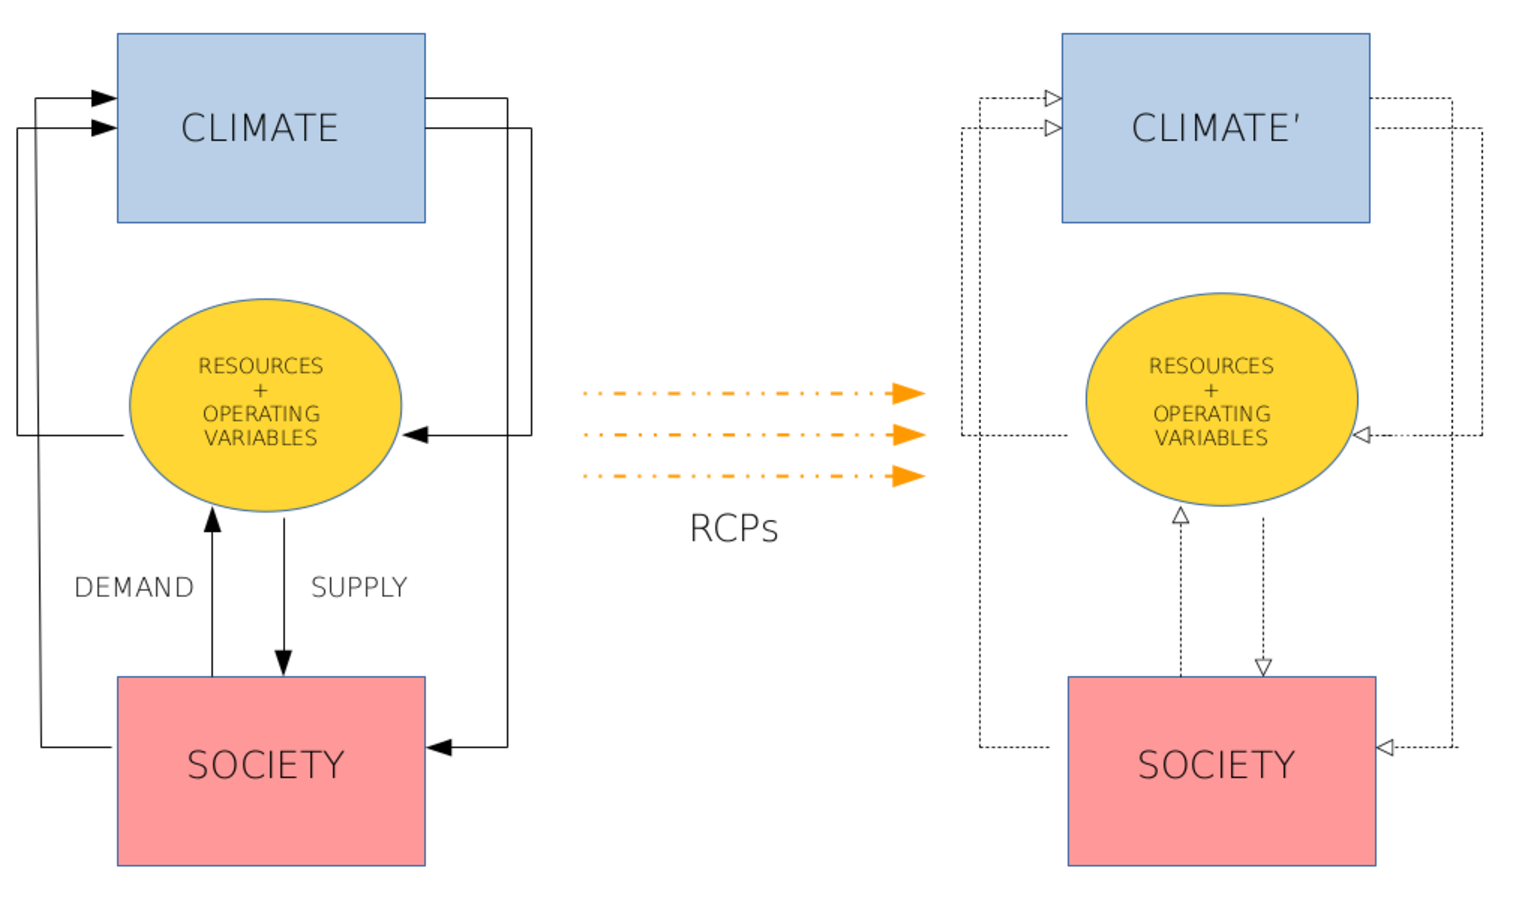
\includegraphics[width=0.6\textwidth]{figs/esquema.pdf}
\caption{Scheme: conceptual representation of the relationships between climate, energy sector and societies. Left side of the scheme represents actual conditions and right side is the future relationships after the evolution following an RCP scenario. }
\label{fig:feedback}
\end{figure}

 
%La bancabilidad[ref] de un proyecto renovable depende de dos factores: en primer lugar su recurso y en segundo lugar, sus beneficios. Los beneficios obtenidos por el proyecto renovable dependerán del periodo de operación y de la cantidad de energía suministrada en este tiempo. Por ello, una evaluación adecuada, no sólo del recurso disponible a lo largo de todo el proyecto, sino de su variabilidad y de las posibles tendencias, es necesario a lo largo del ciclo de vida de la planta, que puede alargarse hasta 30 años[ref].



%En la figura... están representados diversos eventos meteorológicos y climatológicos que afectan a la generación energética. El eje 'x' representa las distintas escalas temporales en las que ocurren estos eventos. Es interesante destacar, aunque no es el tema principal de esta investigación, la relevancia de la escala estacional y sub-estacional para la operación de las plantas energéticas de tipo renovable. La mejora en la predicción climática en estas escalas repercutirá de forma directa en la planificación de la operación y mantenimiento, así como ayuda en la gestión por parte del operador de red y mercado. Por ejemplo, conocer con antelación si un otoño va a ser especialmente lluvioso, sirve para predecir la cantidad de electricidad que se puede producir con las centrales hidroeléctricas, haciendo el sistema mucho más eficiente y fiable. 



% !! escalas climáticas: ¿es importante la repotenciacion? tener en cuenta esto? mismo recurso en el futuro?
% !! infraestructuras y extremos climáticos.


\subsection{Climate services}

%Con la creciente demanda de información por parte del sector energético de predicciones y proyecciones climáticas, aparece de manera natural la creación de los servicios climáticos para sistematizar, de alguna manera la información necesaria para los distintos stakeholders. 

Due to the intrinsic characteristics of renewable energy resources, related to their high space-time variability and the potential impacts on the energy sector mentioned above, there is an increasing demand of information about many climate forecast, projections and hazards. Altough the energy sector is one of the most interested in the development of an operational system of climate information, there are also other sectors that would benefit from that, like agriculture or turism.  
  
This increasing demand of predictions and climate projections from diferent sectors, has lead to the development of the  climate services, in order to systematise, to organise and to target the information for different stakeholders. [ref]

%Como puede observarse en la figure \ref{fig:feedback}, los procesos de interacción entre la sociedad y las variables involucradas en la generación de energía son de doble sentido. Por un lado el abastecimiento dependerá de la disponibilidad de los recursos y por otro, la demanda está directamente influenciada por estos factores climáticos. Teniendo en cuenta esto, el desarrollo de los servicios climáticos debe basar la mejora de sus modelos y por lo tanto, de los productos ofrecidos en estas dos premisas.

From the renewable energies side, climate information is specially relevant for strategic decisions, evaluation risks, planning and trading operations. As can be seen in figure \ref{fig:feedback}, interaction processes between society and the variables involved in the energy generation are two-way relations. On one hand, the energy supply would depend on the availability of the resources and constrains due to climate change;  and on the other hand, demand is directly influenced by those factors. Due to that, development of climate services should be based on the improvement of the models and the offered products considering the two sides.   

%La información climática en el sector energético es especialmente relevante para las descisiones estratégicas y la evaluación de riego, las operaciones de trading o la planficación de la operación y el mantenimiento en las plantas de generación (especialmente) renovables.



%Es relevante, aunque no es el tema de esta tesis, decir que también otros tipos de generación no renovable pueden beneficiarse de esta información y estar afectados de manera importante por algunos eventos climáticos. Por ejemplo, el aumento de temperatura del aire puede provocar una subida en la temperatura de los ríos, que ocasionalmente repercute en la operación de las plantas nucleares. En estos casos, estas plantas se ven afectadas porque no pueden continuar on las operaciones de refrigeración de los reactores (ref). 


%\section{Resource assessment}
\section{Climate change and the Mediterranean area}

% \begin{itemize}
% \item Cambio climático de origen antropogénico a escala global. Aumento de la temperatura global.
% \item Los impactos del cambio climático ocurren en escalas locales o afectan de manera local a distintas comunidades y poblaciones de una forma desigual, relacionada también con su capacidad de adaptación y resiliencia.
% \item Por las razones mencionadas arriba, la respuesta a los diferentes impactos de cambio climático deben adoptarse de manera local, a pesar de que el consenso sobre la urgencia de actuación sea global y se adopten compromisos globales comunes.
% \item La mitigación de los grandes impactos ocurre en escala regional/local.
% \end{itemize}

%El sistema climático ha variado continuamente y de manera significativa a lo largo de la historia de la Tierra. Las variaciones del clima puede explicarse debido a factores o forzamientos externos y la respuesta del sistema climático a los mismos o, por otro lado, puede ser la causa de inestabilidades internas y relaciones no lineales entre los distintos componentes del sistema.

Climate system has varied constantly and significantly along the Earth's history. Climate variability can be explained due to external factors and the response of climate system to them or, on the other hand, due to the internal instabilities and non-linear relationship between different components of the system, occuring the last ones with independence of the external forcings.

%Los distintos forzamientos de origen externo pueden ser factores astronómicos, como los cambios en la intensidad de la radiación solar o en los parámetros orbitales, o bien, factores terrestres como la composición de la atmósfera debido a la actividad humana, cambios en la superficie terrestre debido al uso de la misma etc.

External forcings can be astronomic factors, like changes on the intensity of solar radiation or in the orbital parameters, or they can be terrestrial factors like changes in the composition of the atmosphere due to human activity, changes in the earth's surface due to land use etc.

%Algunas variaciones del sistema climático ocurren de manera independiente de los forzamientos externos. Estas variaciones tienen su origen en las distintas interacciones no lineales entre los componentes del sistema climático y dan como resultado la variabilidad natural del sistema climático. 

%Some variations of the climate system happen independently of the external forcings. These variations have their origin on different no-linear interactions between different components of climate system and the result is the natural variability of the climate system.

%Desde la revolución industrial la Tierra ha experimentado un aumento de la temperatura global que no es posible explicar mediante los forzamientos externos 'naturales'  del clima como cambios en la actividad solar o en las emisiones volcánicas (Bindoff et al, 2013), ni forma parte de la variabilidad natural del sistema. El IPCC en su último informe, asegura que la actividad humana y en concreto las emisiones de efecto invernadero generadas desde la Revolución Industrial (1850) son responsables del cambio climático que ha generado el ascenso de temperatura global y que ha hecho que probablemente los 30 años entre 1983-2012 hayan sido los más cálidos en los últimos 1400 años en el hemisferio norte (IPCC). A pesar de la marcada variabilidad interanual (Stocker et al. 2013), el aumento de temperatura con caracter global en las últimas décadas es evidente. [ref de observaciones globales]

Since the Industrial Revolution the Earth has experimented an increase in the global temperature that cannot be explained due to natural external forcings like changes on solar activity or volcanic emissions (Bindoff et al, 2013), either it cannot be explained as part of the internal variability of the system. The IPCC in its last report, assure that human activity and more precisely, GHG emissions generated since 1850 are responsible of the climate change that causes the increase in global temperature and has made that probably the last 30 years between 1983-2012 have been the warmer in the last 1400 years in the northern hemisphere (IPCC). In spite of the large interannual variability (Stocker et al 2013), the global character of the temperature increase in last decades is clear.[ref de observaciones globales].

%Las consecuencias del aumento de temperatura desde un punto de vista físico dependen de la sensibilidad del sistema a los cambios en la concentración de gases de efecto invernadero. Son numerosos los estudios [ref] que se han realizado para intentar cuantificar el impacto que este aumento de temperatura puede tener en los distintos subsistemas a través de los diferentes mecanísmos de retroalimentación que pueden generarse.

%A pesar de la característica global del cambio climático, sus consecuencias e impactos son percibidos a escala local y regional. Estos impactos afectan a comunidades y poblaciones de manera desigual dependiendo de su capacidad de adaptación y resilencia. Por ello, la respuesta desde un punto de vista socio-económico para mitigar estos efectos, tiene que venir dada en esta escala, aunque exista consenso sobre la urgencia de actuación y se adopten compromisos comunes.

Despite that climate change is a global concept, its consequences and impacts are perceived in a local and regional scale. These hazards and impacts affect communities and population unequally depending on its vulnerability, adaptation capabilities and resilience. Due to that, the socio-economic response to mitigate climate change impacts has to be applied in that scale although it should be a consensus on the urgency and some common compromises have to be adopted.

%Uno de los primeros trabajos que intentaba cuantificar el impacto del cambio climático a escala local fue el de Giorgi et. al 2006. En este trabajo, se utilizaba por primera vez un índice (RCCI) para medir de forma cuantitativa y compara geográficamente las zonas más afectadas por el CC. En este aspecto, el trabajo estaba enfocado desde un punto de vista climático, es decir, el índice mide la sensibilidad del clima en esa zona. En este sentido, el Mediterráneo aparecía como una de las zonas más afectadas y desde entonces ha sido denominado como un hot-spot de CC.

One of the first works on quantification of climate change impacts in a regional scale was the one published by Giorgi in 2006 \cite*{Giorgi2006}. They used for the first time an index, RCCI, to measure and compare geographically the climate sensitivity of different areas to climate change. The conclusion of the research showed the Mediterranean area as on of the most affected area in terms of climate response to climate change, and since then it has been refered to as a climate change hot-spot.

%Los ensembles de modelos climáticos proyectan escenarios en los que las principales consecuencias del calentamiento global en el área Mediterránea son un descenso generalizado de las precipitaciones, debido a un aumento de la circulación anticiclónica asociada a un desplazamiento hacia el norte de ``Atlantic storm track''. Las temperaturas proyectadas son inusualmente altas con un ascenso especialmente alto en los meses de verano.

The climate models projects scenarios in which the main consequences of global warming in the Mediterranean area are a generalised decrease of precipitations (with the exception of some areas like the Alps), due to an increase in the anticyclonic circulation, that is associated with a northward shift of the Atlantic storm track [ref]. Also it is projected an increase in interannual variability of temperature and precipitation, mostly in the warm season \cite*{Giorgi2008}. In terms of extreme events, it is also projected less frequent but more intense precipitation events and with respect of temperature, some authors have evaluated the probability of an increase in heatwaves over the Mediterranean area [ref]. All this climatological perspectives, consequencies of the global warming,  should be considered in order to plan and prepare the adaptive capacity of the region.\\   

\section{Organization of the manuscript}%\section{General scientific question: spatiotemporal variability of solar resource and photovoltaic production}

This manuscript is organised as follows:

The \textbf{first part} of the text contains two chapters: the first one is the previous \textbf{Introduction}, that aims to introduce the context in which the thesis has been elaborated. In the second chapter, \textbf{State of knowledge}, there is an introduction on the main contributions related to this topic over the literature. It includes a general overview about intermittency of PV and how the short-term problems has been managed. After that, the long-term problems and the main contributions about this topic over the area are reviewed. %Also, the climate change perspective over the Mediterranean region and the main literature related to solar resource is revised.

The \textbf{second part} is composed by two chapters including the \textbf{Data} description and the \textbf{Methodology} used along the studies. In this case it is important to remark that each results chapter has its own 'Data and Methodology' section used for that specific chapter. The contents of this part II are related to general description of ground stations, satellite, climate data and models as well as general methodologies.

The \textbf{results} are presented in the \textbf{third part} of this manuscript. There is a different chapter for one of the main aspects investigated here and described in the above section. The organisation of this chapter is being adapted from the journal papers where these results have been published.

Finally the \textbf{fourth part} contains a chapter with some \textbf{discussion} and limitations about the results previously presented and the main \textbf{conclusions}. This section also summarises the main questions emerged from the work, which will lead future research.

% \section{State of the art}
% \subsection{From short to long term varibility issues}
% \subsection{Solar radiation data measurements}
% \subsection{Satellite data}
% \subsection{Modelization of solar radiation}
% \section{Identification of knowdlege gaps and approach to the problem}
%\subsection{Spatiotemporal long-term variability in an almost isolated area}
%\subsection{Role of aerosols in the spatiotemporal varibility of the photovoltaic energy production}
%\subsection{Future availability of photovoltaic potential}

 
\chapter{State of knowledge\label{cha:state}}

\epigraphfontsize{\small\itshape}
\epigraph{''Commençons par les systèmes les plus simples et les plus faciles à cerner pour monter graduellement à la compréhension des plus complexes.''}{--- \textup{René Descartes}, Le Discours de la Méthode}

\section{Variable renewable energies: VRE}

The variable nature of renewable energy resources, in space and time, is a key aspect for their high penetration into the conventionally designed electricity systems. Due to the requirement that supply and demand have to match at every time-step, the forecast and management of the generated electricity is needed for accomplishing this match, which becomes more difficult in the case of variable renewable energy (VRE) plants.

In the traditional electricity systems, a portfolio of centralised power plants (coal, nuclear, gas...) dispatches electricity as the customer loads demand it. The conventional power plants are able to storage the primary energy that they use and produce electricity only when it is needed. With the increase of renewable power plants, mostly wind and solar, the supply of electricity demand approach has changed. The VRE power plants only produce electricity when enough resource is available and in the case of photovoltaic power plants, only during the daylight time. This concept has being refered as \textbf{intermittency}, to recall the fact that solar and wind resources are not available at any time and that they are variable by nature. Nevertheless, there are renewable power plants that are able to provide energy by demand, like biomass power plants or hydropower (with some restrictions in drought events). They are dispachable and can operate as the conventional thermal power plants.

Due to the rising penetration of the non-dispachable power plants (wind and solar) the management  and the operation of the system has to be adapted. However, the alternatives for energy storage for VRE plants are increasing in different ways: batteries for wind and photovoltaic power plants, hydrogen or pumping hydro-power \cite*{Lund2015, Blanco2018, Schaber2004}, which favours the integrations of the alternative energy sources.

The research in storage for VRE is rising but different approaches are also being adopted to integrate high share of this alternative technologies. The term \textbf{flexibility} is one of the most used refered to the new strategies followed from the demand and supply side in order to adapt to the new system \cite*{KROPOSKI2017}. From the demand side, flexibility refers to means related to load shape and demand patterns, like peak saving, load shifting, valley filling etc \cite*{Lund2015}.

On the other hand, flexibility of the supply side depends on the power plants, whose output can be controled to obtain power balance. It is important in terms of flexibility to consider the response time of different power plants as well as the different nature of each one. As the availability of solar and wind resources are not related to the geographical distribution of the demand, a highly interconnected grid is one of the main needs for a high penetration of VRE. Once this is considered, geographically spread portfolio of VRE plants are able to smooth variability of power output \cite*{KROPOSKI2017, Marcos2012}(Hoff and Perez 2012, 2013, añadir más referencias).

%* Explicar más el concepto de smoothing?? agregar aquí todas las citas de smoothing

There are also studies that try to identify complementary features of different energy resources, either in time or in space, in order to address the intermittency issue through the smooth of the total power output. The complementary studies are made using different technologies like hydro-power and wind power \cite*{Denault2009, Silva2016} or hydro-power and solar photovoltaic \cite*{Francois2016, Beluco2012, Kougias2016}. In \cite*{Hoicka2011} complementary of wind and solar is investigated for a region in Canada and also in Italy \cite*{Monforti2014}.  In addition, over the Iberian Peninsula \cite*{Santos-Alamillos2012, Jerez2013b} and Great Britain \cite*{Bett2016} it has also being investigated from a more climatological approach.

As much as we were able to forecast the variability of solar/wind resources in the short term and in to characterize the resource in the long-term to  estimates and project the energy to be produced, better flexibility measures and strategies could be apply to integrate high rates of VRE without compromise reliable and efficiency.

% For example on the supply side, the kind of flexibility is accomplished through power plants with
% different response time. Introducing variable power generation such as wind and solar power may
% increase the need of energy system flexibility, which could be accomplished through additional measures
% on the supply or/and demand side which is the subject of this paper. From the electricity system point of
% view, flexibility relates closely to grid frequency and voltage control, delivery uncertainty and variability
% and power ramping rates
\section{Variability sources in PV}

It is important to notice that every power system has associated an inherent variability and uncertainty, as a non-exclusive characteristic of a renewable energy system. In the case of PV systems, the variability of PV outputs depends on two items: on the first place, it depends on the variability linked to the solar irradiation reaching the generator (resource variability), and secondly, it also depends on the behaviour of the electrical components.   

% ``Before focusing on the variability and uncertainty of PV plants, it is important to understand that
% variability and uncertainty are inherent characteristics of power systems. Loads, power lines,
% and generator availability and performance all have a degree of variability and uncertainty
% It is clear that uncertainty in photovoltaic power it is a combination of the uncertainty of estimation of solar resource and the uncertainty in the behaviour of the electrical componentes of the photovoltaic system.''
Solar radiation varies in multiple time-scales, from seconds to multi-decadal variations, as well as spatially, affecting PV production. For the operating activities in PV plants, an accurate forecasting of solar irradiation, which means, being able to reproduce its short-term variabilty, leads to better forecasting of the PV output, demanded by TSOs and used for trading. In longer time-scales, to understand variability features improves the projection of the PV output for a period of time: seasonal, year-to-year produced energy, multi-year trends or climate change projections. That helps in the plannification, the strategy, the financing activities, and can influence in the polycimakers decisions.

Different factors are responsible of the variability either of solar resource or the electrical components of the PV generator and affect them across different time and spatial scales.

\subsection{Astronomical factors}

The amount of solar energy that reaches the photovoltaic generator depends on the first place on the sun position with respect to the orientation of the PV panels, which is a deterministic factor that only depends on the time of the year, the time of the day and the relative position of the generator surface. It means that the first factor causing PV intermittency is the fact that no energy can be produced during night-time. However, although this daily scale intermittency is the one that most affects the PV power production there is no uncertainty associated to this fact, which is a very important concept in order to manage VRE.

\subsection{Atmospheric factors}

\subsubsection{Clouds}

There are other factors that reduce the amount of solar energy reaching the surface and their influence depend on the composition of the atmosphere at each time. When solar radiation goes through the atmosphere it can be reflected, absorbed or scattered. The presence of clouds is the most affecting factor in the transmission of solar radiation to the surface. The condensed particles that forms clouds makes solar radiation being scattered and reflected and part of the radiation can also be absorbed. Different types of clouds affects differently to solar radiation \cite*{Page2012}. High thin clouds are less dense than low clouds, becoming more transparent to solar radiation \cite*{Kasten1980}. %Also, some clouds are less spatially aggregated than others. When the sky is overcasted, the amount of energy reaching the surface decrease but the frequency of the intermittency generated in the PV output is not as high as if some individual clouds pass through.

For partially cloudy skies, solar irradiance (direct component) can drop in seconds \cite*{Page2012} due to clouds. In overcasted periods, shorth-term variations depends on the tipe of clouds.

Low frequency changes in cloud cover for large areas are related to changes in large scale circulation patterns, which is linked to changes in solar resource for that places \cite*{Chiacchio2010, Sanchez-Lorenzo2009}.

%{\color{blue} Incluir referencia del libro: practical handbook of photovoltaics funcdamentals and applications para tipos de nubes y su transmitancia y otras referencias}
\subsubsection{Aerosols}

Aerosols is the term used to refered to the solid particles suspended on gas. In this work we are refering to the atmospheric aerosols, which are the solid particles suspended on the atmosphere but the hydrometheors like ice crystals \cite*{boucher2015}. In the absence of clouds, aerosols are the main source of variability for solar resource. 

Aerosols impact solar radiation in two ways: directly, scattering, absorbing or reflecting solar radiation or indirectly, acting as condensation nuclei favouring the formation of clouds \cite*{boucher2015}. They can be classified depending on its source origin. Natural sources emit aerosols from oceans, wild fires and vegetation, whereas antrophogenic sources emit aerosols from industrial activities, burning fuels and human-caused fires.

%  Natural sources consist of emissions from
% the ocean, soils, vegetation, fires, and volcanoes. Anthropogenic sources are
% largely dominated by emissions from the combustion of fossil fuels (i.e. coal
% and oil), biofuels (plant biomass including wood, vegetable oils, animal waste),
% other fuels (e.g. peat), or vegetation fires caused by humans. Industrial activities,
% transportation, heating, or even domestic activities related to cooking in developing
% countries, are important sources of aerosol

Aerosols vary greatly in time and accross space \cite*{Kaufman2002}. Besides of aerosols relatively short residence time in the atmosphere (of the order of hours to weeks), they have an strong influence on climate through their impat on the radiative budget and clouds \cite*{Nabat2015, Nabat2015a}. Aerosols from natural sources, like mineral dust airbons, which last some days, have a very strong seasonality, affecting in regional and continental scales periodically.  Also, due to the relationship between aerosols and human activities, long time cooling trends have been detected in China for last decades related to the increase in aerosols optical thickness (Giorgi 2002) and other studies had shown the relationships between the ``dimming'' and ``brightening'' and the antrophogenic aerosols emissions \cite*{Wild2005, Wild2012, Wild2009}. 

%{\color{blue} Falta incluir referencias: A satellite view of aerosols in the climate system Kauffman 2002}
%Gueymard, C.A. Temporal variability in direct and global irradiance at various time scales as affected by
%aerosols. Solar Energy 2012, 86, 3544 – 3553.

\subsection{PV system factors}

\subsubsection{Spatial aggregation}

There are two factors related to the spatial dimension that influence on the photovoltaic power variability:

\begin{itemize}
\item {Power plant size}
  A PV power plant acts like a low-pass filter for short-fluctuations, which means that higher frequencies of power fluctuations (less than a minute) from the PV generator are smoothed as a function of the PV plant size \cite*{Perpinan2011, Perpinan2013}.
\item {Distance between power plants}
  On the other hand, it has been also concluded that for a fleet of dispersed PV plants, ahort-term power output fluctuations are attenuated. Some authors observed thar short-term fluctuations are essentially uncorrelated for distances between PV plants over 6 km.\cite*{Otani1997, Wiemken2001, Hoff2012}
\end{itemize}

%{\color{red}Another important factor that affects PV output fed into the grid is the PV generator size or even distance between different PV power plants. In the short and very short time scales,  This is called te smoothing effect and it can be used as one of the strategies to follow in order to address the variability issue of renewables.}

\subsubsection{Other factors}

As it has been noted at the beginning of the section, there are other factors that affects the performance of a PV system, causing variations in the power output. These factors are related to the electrical components of the system and they can be divided into internal and external facors.

The most important external factor affecting the PV system is temperature. It affects cells performance and if temperature is highly different than the optimun cell temperature the efficiency will drop. Also some external factors like dust deposition can affect the electrical performance, limiting the energy reaching the cell \cite*{Fan1986, Mekhilef2012,Dubey2013}.

Internal factors affecting the PV output that can cause variability are related to the transmission lines, wires and interconnections, or the inversor, whose functioning is not always constant and can present variations.

\section{Short-term variability}%Photovolatic power forecasting

%Considerando los distintos factores que intervienen en la variabilidad de la producción fortovoltaica antes mencionados, queda reflejado que el estudio de la variabilidad puede hacerse bien desde el punto de vista del recurso, es decir, de la radiación solar en superficie o incidente en el generador, o bien desde el punto de vista de la generación eléctrica.[widen]

From the different factors that influence in variability of PV power production, it can be followed that variability studies can be made through the solar \textbf{resource} point of view or from the \textbf{power} variability side \cite*{Widen2015}.
%El estudio de la variabilidad a corto plazo desde el punto de vista del recurso ha venido ligado a la ivestigación sobre la caracterización del la radiación solar en superficie. Algunos de estos estudios tenían como objetivo únicamente el modelado estadístico del comportamiento de la radición en escalas temporales cortas [Liu] y otros estaban motivados por el desarrollo de la energía solar fotovoltaica y la necesidad de caracterizar el recurso para el mejor funcionamiento de las mismas.[collares pereira] 
%{\color{blue} HAY QUE METER VARIABILIDAD POR AEROSOLES}

\subsection{Resource Variability}

% El estudio de la variabilidad a corto plazo desde el punto de vista del recurso ha venido ligado a la ivestigación sobre la caracterización del la radiación solar en superficie. Algunos de estos estudios tenían como objetivo el modelado estadístico del comportamiento de la radiación en superficie en escalas temporales cortas [Liu] y otros estaban motivados por el desarrollo de la energía solar fotovoltaica y la necesidad de caracterizar el recurso para el mejor funcionamiento de las mismas.[collares pereira] En este sentido, el estudio de variabilidad ha sido generalmente de carácter local.

The research of short-term variability from the resource perspective, has followed the research about the characterization of solar irradiation at the surface. Those studies had the objective of the statistical modeling of solar irradiation behaviour at the Earth's surface in shor-term time scales \cite*{Liu1960}. Others, were motivated by the solar energy development and the need of characterize the resource for a better performance of the PV plants \cite*{Collares-Pereira1979}. In that sense, variability studies has been generally focused with a local character.

%{\color{red}Para las distintas operaciones en el corto plazo, predecir la cantidad de energía que un generador o planta fotovoltaica va a verter a red, ayuda a a la gestión de la intermitencia inherente a la producción fotovoltaica. Para ello, será necesario en primer lugar predecir la energía solar incidente en el generador fotovoltaico y en segundo lugar modelar el comportamiento del generador fotovoltaico para predecir la AC producida.}

For different operation activities, to forecast the amount of energy fed into the grid from a PV system or plant, is essential in order to manage the associated intermittency to the photovoltaic power production. In order to acomplish that, it is needed on the first place to forecast the amount of incident solar energy on the photovoltaic generator and secondly, to model the system's behaviour in order to forecast the AC produced.   

%lleva a analizar PV production 'ramps' provocadas por cambios en la radiación solar incidente asociados al movimiento de nubes y el efecto 'smoothing' antes mencionado. En este aspecto, la escala temporal está relacionada con el grado de 'suavidad' que se puede alcanzar con la agregación espacial de distintas plantas fotovoltaicas.

% Por otro lado, el tamaño del generador es un factor que ha sido estudiado para determinar la variabilidad en escalas de tiempo entre tal y tal, observándose que :

% he main research question in current solar variability research is which degree of smoothing of the intra-hourly fluctuations can be achieved with different degrees of geographical dispersion of irradiance sensors or PV systems (see Section 4.4). Current research efforts are in particular focused on determining the relationships between cloud speeds, correlations between sites, time resolution and overall variability. Previous overviews of the field can be found e.g. in [1,8,70,71]. The time scales focused on in current research on solar variability range from several minutes down to seconds. The
% relevant time scale depends on the correlation between these sites, which in turn depends on the distances between them. The shorter the time scale, the faster the decline in correlation. Determining the variability for completely correlated or uncorrelated ensembles of systems is straightforward [72], while the range in-between is non-trivial. For example, [70,73,74] and other studies indicate that close-to-zero correlation is reached at a few up to tens of km for resolutions of seconds or minutes, which is the spatial and temporal scale least explored in existing research
% [70,75].

% Also, the smoothing effect that a well-spread site planning has on the PV production is being investigated: [Mar+12], [PML13].

 
%{\color{red} Como se ha comentado anteriormente, para las distintas operaciones en el corto plazo, predecir la cantidad de energía que un generador o planta fotovoltaica va a verter a red, ayuda a a la gestión de la intermitencia inherente a la producción fotovoltaica. Para ello, será necesatio en primer lugar predecir la energía solar incidente en el generador fotovoltaico y en segundo lugar modelar el comportamiento del generador fotovoltaico para predecir la AC producida.}
  
%The energy that is obtained from a photovoltaic system can be forecasted in advance if the amount of solar energy that reach the generator surface is accurately predicted. The prediction of solar irradiation variability enhance the forecast of the energy output. After that, it is necessary to model the electical components of PV generator. 

%%%%%%%%%%%% ELimino esto porque es un lío con lo de clear sky pero tengo que coger alguna referencia (Tovar)%%%%
%There are different types of forecasting methods for solar power, they are based on the models that forecast solar irradiation. Among them there are two different approaches: \textbf{physical methods} and \textbf{statistical methods}. Physical methods are based on the radiative transfer equation and physic variables whereas the statistical or empirical methods are based on historical data. Some approaches are also \textbf{hybrid} approaches that combined both \cite*{Diagne2013, Tovar-Pescador2008}. They mainly rely on two principles: first an estimation of the clear-sky irradiance and secondly, they account for the presence of clouds [ref Jan Kleiss].  


\subsubsection{Solar irradiation forecasting}

There are different types of forecasting methods for solar irradiation. There are two different approaches: \textbf{physical methods} and \textbf{statistical methods}. Physical methods are based on the radiative transfer equation and physic variables whereas the statistical or empirical methods are based on historical data.

The application of each kind of the forecasting models is very related to the \textbf{forecast horizon} that want to be addressed, as well as the horizontal resolution. In the operation activities, 3 time forecasting horizons were described by Kostylev and Palovsky \cite*{kostylev2011solar}: intra-hour, intra-day, day-ahead. For other activities like trading, the day-ahead forecast is very important as well as for planning operations. The statistical approach is applied in shorter scales whereas the physical approach has been proved to have a better performance \cite*{Perez2010, Diagne2013, Widen2015}.% in longer time-scales seasonal forecast will be a very valuable asset if model skill improves [ref]. 

\begin{itemize}
\item{Physical Methods}

The physical modeling of solar radiation is based on physical equations of the interaction between atmospheric components and solar radiation (aerosols, water vapour, clouds...). When solar radiation goes through the atmosphere, it can interact with its components being absorbed by molecules, back-scattered to space or scattered in any other direction. Thus, only part of the solar radiation at the top of the atmosphere (TOA) will reach the Earth's surface.

This process is the physical process of energy transfer described by the radiative transfer equation (RTE) and its solution needs a radiative transfer model (RTM). The radiative transfer is a very complex process that needs to be simplified to be solved numerically and some parametrizations are needed. However, from these models it is possible to reproduce the solar radiation behaviour across the atmosphere and at the surface. RTMs are in the core of numerical weather prediction models, NWP, and climate models and sometimes they are used to obtain solar radiation from satellite images, although in this case empirical or semi-empirical approaches are also commonly applied.

Numerical weather prediction models are very useful in a time range from 4h to 6h and they are also applied for the day-ahead forecast \cite*{Perez2010}. It is very frequent to apply a post-processing process to the output of NWP that enhance the forecast. Some statistical tools like bias correction can be apply to reduce some systematic errors or local effects \cite*{Diagne2013}.

%{\color{red} Introducir aquí que en el desarrollo de NWP no se han incluido aerosoles ?}

\item{Statistical methods}

Solar radiation at the surface can be estimated also using statistical methods. In this case it is necessary to have enough accuarate historical data to create and validate the model and likely these models will not be able to reproduce solar behaviour universally. However, they can be very useful for local applications and at very high time-resolution.

Under these methods traditionally used to forecast time-series, relies the idea of predict some variables throught the statistical analysis of historical data and its relationship with other variables called predictors. Many models have been developed in this sense from the most simple approach, the persistence model or autorregressive models, to more sophisticated ones \cite*{Reikard2009, bacher2009, Inman2013}. Also, with the develop of the ANN, non-linear models have been also applied to solar the forecasting field, withthe predictions based on an algorithm learning \cite{Mellit2008}. 
 
%{\color{red} escalas temporales: short term and very short-term. Se analiza el impacto de las nubes -> muy común aplicar un modelo de cielo claro y después la influencia de las nubes. Describir aquí lo que son los modelos de cielo claro?}

%{\color{blue} meter aquí clear-sky models? y que pasa con los de satélite}


% Statistical methods have been used successfully in time series forecasting for
% several decades. Using the statistical approach, relations between predictors,
% variables used as an input to the statistical model, and the variable to be predicted,
% are derived from statistical analysis. Several studies with respect to
% direct time series modeling have been performed. In Reikard [2], different time
% series models are compared. In Bacher and al.[7], the authors investigate the
% use of a simpler AR model to directly predict PV power in comparison with
% other models.

\item{Hybrid methods}

It is very common to apply a combination of more than one model to enhance the prediction accuracy. Many studies have shown the overcome of a combination of two different approaches with respect to a simpler approach \cite*{Diagne2017, Yang2014}. For instance, some studies show the application of ANN methods after the obtention of NWP output \cite*{Cornaro2015} or after obtain a satellite-based model output \cite*{Marquez2013} 

\begin{figure}[h!]
\centering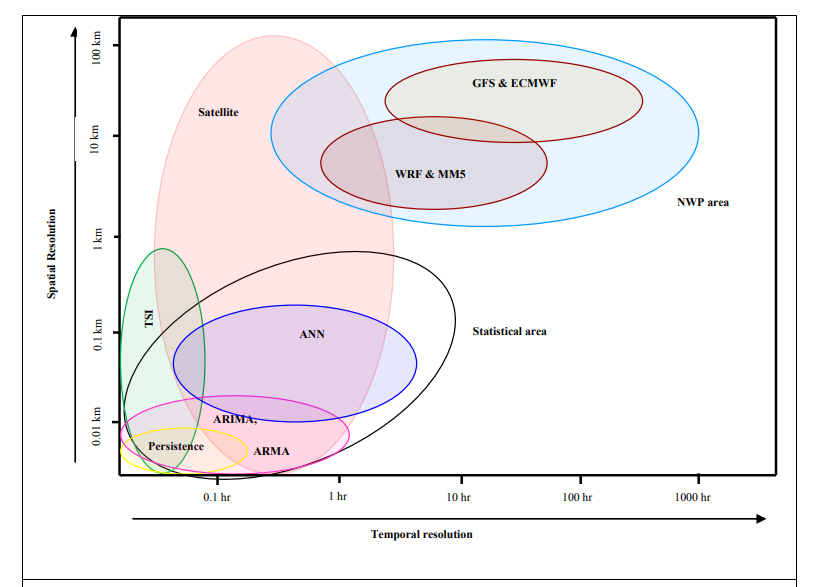
\includegraphics[width=0.6\textwidth]{figs/forecast.png}
\caption{Models to forecast irradiance depending on the time horizon. Incluir ref aunque se va a rehacer}
\label{fig:forecast}
\end{figure}


Different models are applied depending on the forecast horizon as they are summarised in the figure. For shorter periods, statistical methods are prefered to derive solar irradiation from satellite measurements. As far as the time horizon increases, the NWP are used to forecast irradiance.

%Usually, the main steps in the solar irradiation forecast are first the estimation of the clear-sky irradiance and after that account for the presence of clouds ref[Jan Kleiss].

\end{itemize}

\subsubsection{Aerosols in solar irradiation forecasting}

Although clouds are the main driver of variability of solar resource, under cloudless conditions, aerosols reduce the amount of solar energy reaching the earth's surface. Some models compute solar irradiance in clear sky conditions, which means that the they calculate attenuation of solar irradiation only due to the constituents of the atmosphere. Many clear-sky models has been proposed on the literature \cite*{Gueymard2012}. The difference between clear-sky models is based on the parameters used to predict solar irradiance. The most simplest ones only consider the zenith angle and extraterrestrial irradiation. The higher the complexity of the model, the more parameters are included to characterise the state of the atmosphere: different aerosols content, water vapour etc. Performance of this models depends on the parametrizations of each model and the knowdlege of the atmospheric composition.
 
These models are commonly used in to derive solar irradiation from satellite observations (see chapter data). As satellite are able to give observations of the cloudiness at a given time and site, the use of a clear sky model in combination with this sobservation make easy to establish a relationship between the cloud index and the clear sky index . The role of aerosols input in these satellite-based methods to derived solar irradiation has been investigated in \cite*{Polo2014}. 

On the other side, under high loads of AOD, NWP usually presents a systematic bias in solar radiation forecast \cite*{Rieger2017}. This fact is due to the design of the models that normally use climatological values for the representation of aerosols with homogeneous spatially and temporally concentrations. This fact lead to an overstimation of solar irradiation in the dust outbreak of 4 april 2014 in Germany, which caused significant economic losses \cite{Rieger2017}.

%{\color{blue} Aquí podemos hablar de los aerosoles, que impactan en la predicción de la irradiancia porque afectan a su variabilidad. Númerosos métodos de NWP están desarrollando módulos para tener en cuenta los aerosoles. Por otro lado, estos pueden ser tenidos en cuenta en los modelos estadísticos como predictores. Un buen ejemplo son los modelos de cielo claro, que estiman la radicaciónn en condiciones de cloudless, por lo que los aerosoles son el factor determinante. En este caso, únicamente una buena representación de los aerosoles puede dar un buen valor de la radiación solar en superficie.}\\

%{\color{blue}Sensitivity of satellite-based methods for deriving solar radiation to different choice of aerosol input and models}\\

%{\color{blue}Impact of the 4 April 2014 Saharan dust outbreak on the photovoltaic power generation in Germany}
% incorporates two or more techniques and produces a new
% forecasting method with improved accuracy. In this method
% the deficiencies of the individual model are overcome and
% advantages of individual models are utilized. These methods
% also reduce the forecast errors. For evaluating the forecast
% errors solar forecasting evaluation metrics are also studied.
% Forecasting evaluation metrics allow to understand how much
% to trust the forecast and re-evaluate it in case of high errors.

% \subsection{Clear-sky models}

% Among the different approaches to model or forecast solar irradiation at the surface clear-sky models deserves special attention. These models estimate solar irradiation under clear-sky conditions, which means that the attenuation of solar irradiation is only due to the constituents of the atmosphere and not due to clouds.

% The difference between clear-sky models is based on the parameters used to predict solar irradiance. The most simplest ones only consider the zenith angle and extraterrestrial irradiation. The higher the complexity of the model, the more parameters are included to characterise the state of the atmosphere: different aerosols content, water vapour etc. 
% The amount of energy that reaches the surface depends on the transmittance of the atmosphere. The incident extraterrestrial irradiance at the top of the atmosphere (TOA) would be attenuated depending on the composition of the atmosphere thus in the air mass (AM) crossed to reach the surface. For the latter reason, the zenith angle is the first factor to consider when the surface solar irradiation want to be estimated: with higher zenith angles, higher the air mass. The simplest models based on this parameters are empirical relationships based on measurements for an specific location. Evaluations of these models have shown that it is necessary to take care when applying for a different location that the one used for its calibration \cite*{Badescu1997, Davies1989}.

% In addition to these simple models, some parameters can be considered enhancing the performance of the forecast. The Kasten model [] and the Inchen and Perez [] (that is a modification of the first one) use the zenith angle, the air mass, the elevation and the the Linke turbidity, a parameter that describes the optical thickness of the atmosphere.

% The most sophisticated clear-sky models includes more parameters like the ozone, aerosols and precipitable water. Some of the most used models are Bird, MAC, or REST2[]. There are several studies that summarises a benchmark of different clear-sky models \cite*{Gueymard2013a,b}. It is clear that there is a relationship between the more atmospheric variables included in the model, the better the performance. But measures of all variables included are not always available. Due to that reason, the best model would arise from a balance relationship between the availability of atmospheric measurements to calibrate the model and its performance. 
 
% Referencia para esta clasifion: Global Horizontal Irradiance Clear Sky Models: Implementation and Analysis

%\subsection{Satellite-based models}

% Due to the scarcity of solar radiation measurements, the availability of satellite data has become an important trigger for the development of targeted products for the solar industry [ref].

% There are different methods to retrieve solar radiation from satellite images that goes from physical models to empirical ones. In the first case, the models try to explain the radiance observed by the satellite instrumentation with a radiation transfer model (RTM). In order to do that, it is necessary to know the composition of the atmosphere. On the other hand, empirical models are based on simple regression models between the visible-channel's recorded intensity and grounded measurements. 

% It is possible to extract cloudiness information from the satellite radiance information due to the fact that intensity of the measurements change depending on the composition of the atmosphere and the cloud cover. Considering that, a simple equation can describe the relationship between the radiance measured and the amount of clouds, this was called \textbf{cloud index [Cano].}

% To retrieve solar radiation form satellites, most empirical methods considers a linear relationship between the cloud index and atmospheric transmittance \cite*{Polo2008} [Polo libro, (Cano et al. 1986; Diabaté et al. 1988; Schmetz. 1989; Diabaté et al. 1989; Noia et al. 1993a; Ineichen and Perez. 1999; Zelenka et al. 1999; Perez 2002; Rigollier et al. 2004; Zarzalejo et al. 2005)].  

% %* cloud index?
% %* clear sky index ?

% There are also some approaches that are in between theses two sides: the semi-empirical models, which have become the most common approach \cite*{Polo2008}. They use a simple radiative-transfer scheme and some statistical regressions between data from satellite sensors and observed data (Schmetz (1989), Noia et al. (1993), Pinker et al. (1995), Zelenka (2001), and Hammer et al (2003)).\footnote{Jan Kleiss, Solar Energy Forecasting and Resource assessment, pp.22.23}

% % The importance of the cloud index concept bases on the fact that satellite
% % information (basically cloud cover information) can be related with the solar irradi-
% % ance incoming to the earth surface. Consequently, most empirical/statistical method-
% % ologies to retrieve solar irradiance from satellite images rely on the assumption
% % of linear relationship between the atmospheric transmittance and the cloud index
% % (Cano et al. 1986; Diabaté et al. 1988; Schmetz. 1989; Diabaté et al. 1989; Noia
% % et al. 1993a; Ineichen and Perez. 1999; Zelenka et al. 1999; Perez 2002; Rigollier
% % et al. 2004; Zarzalejo et al. 2005).


% There are two types of satellites orbiting the earth: The polar orbiting, closer to the earth surface,  with high spatial resolution but limitations in the temporal coverage, and the geostationary satellites (~36000km from the earth's surface) with high spatial and temporal resolution. This last kind of satellites are the commonly used to derived solar radiation at the surface.

% The uncertainty in the satellite radiation estimation comes from different sources. First, Sun elevation affects the determination of clouds position due to the increase of reflections, increasing  the uncertainty for low Sun elevation. Other factors are related to geographical factors. The high albedo of some surfaces like desserts or ice areas makes difficult the determination of clouds, increasing uncertainty (Cebecauer et al. 2011).


% % Physical methods are those based on atmospheric data such as temperature, pressure
% % The physical method is based on the numerical weather
% % prediction (NWP), cloud observations by satellite or Total Sky
% % Imager (TSI) or atmosphere by using physical data such as
% % temperature, pressure, humidity and cloud cover.

% % Nowadays, the most used method is the hybrid method which
% % incorporates two or more techniques and produces a new
% % forecasting method with improved accuracy. In this method
% % the deficiencies of the individual model are overcome and
% % advantages of individual models are utilized. These methods
% % also reduce the forecast errors. For evaluating the forecast
% % errors solar forecasting evaluation metrics are also studied.
% % Forecasting evaluation metrics allow to understand how much
% % to trust the forecast and re-evaluate it in case of high errors.
% % \subsection{Physical methods}

% % \subsection{Statistical methods}
% % \subsection{Hybrid methods}

% % ``For non-concentrating systems (such as most PV systems),
% % primarily the global irradiance (GI = diffuse + DNI) on a tilted
% % surface is required which is less sensitive to errors in DNI
% % since a reduction in clear sky DNI usually results in an
% % increase in the diffuse irradiance. Power output of PV systems
% % is primarily a function of GHI. For higher accuracy, forecast
% % of PV panel temperature are needed to account for the (weak)
% % dependence of solar conversion efficiency on PV panel
% % temperature.''

%{\color{red} PV forecasting methods: parametrics, non-parametrics}
\subsection{PV variability}
\subsubsection{PV power forecasting methods}

Once the solar radiation is either modeled or measured, the AC output from a PV system can be modeled following two main principles \cite*{Almeida2015}:

\begin{itemize}
\item Parametric models
\item Nonparametric models
\end{itemize}

In the first place, \textbf{parametric models} are a set of equations that model each step of the electricity generation: decomposition of solar irradiation in different components, its transposition to the tilt panel of the generator, the behaviour of the PV generator and the inverter to finally get the electricity output. The advantage of this type of models is that can be applied idependently to each loaction. This approach is been used for many authors \cite*{Bofinger2006, Lorenz2008, Lorenz2011} with differences in the sub-models applied in each case.

The \textbf{nonparametric models}, on the other hand, consider the whole PV system as a black box and only takes into account the input data (variables as solar irradiation and temperature) and output historical data, developing an statistical model from the measured values. The constrains related to this approach is that this method can only be applied when the historical time-series are long enough to be representative of the PV plant \cite*{Bacher2009}. 

\subsubsection{Smoothing effect}

Variability of PV production from an individual power plant or from a cluster of them, can be apprach from the perspective of what is been called ``smoothing effect''. This refers to the before mentioned factor that affects variability, the spatial aggregation of the considered units. Whereas the power output of a PV system varies highly in time, the power time series of a group of inverters spatially dispersed is less noisy than the individual series. The same could happen to the aggregation of PV power plants allocated in different places. Therefore, intermittency can be addresed from the study of this two factors:

\begin{itemize}
\item{Generator size}
\item{Distance between power plants}
\end{itemize}

\subsubsection{Aerosols}

The impact of aerosols in photovoltaic energy production has been also studied from the power side. In the short-term, some  extreme events like dust outbreaks has been analysed, due to the impact on a daily basis that they have in PV production. Some authors have seen reductions of PV production in semi-arid regions up to $48\%$ , like the Sahel zone \cite*{Neher2017}. For the western mediterranean, the impact of two extreme events of high loads of dust in one side and smoke on the other were studied and they showed a reduction of $34\%$ for smoke and $6\%$ for dust on daily averages \cite*{Gomez-Amo2019}. For larger areas, the impact of en extreme event in April 2014 over Germany, shows that aerosols could reduce PV production in a country causing large economic losses if these events are not previously forecasted \cite*{Rieger2017}.

%El paper de 2018 del impacto de los aerosoles en de polvo y humo en valencia [Empirical estimates of the radiative impact of unusually extreme dust and wildfire episode on the performance of a photovoltaic plant in the western mediterranean}.
%Por otro lado, estudiar la variabilidad desde el punto de vista de la producción, se ha hecho desde un punto de vista local para analizar PV production 'ramps' provocadas por cambios en la radiación solar incidente asociados al movimiento de nubes o distintos factores.

\section{From short to long term issues}%Photovoltaic power projections}%{}

Despite the variable behavior of surface radiation in the short-term, there was a belief that solar radiation was stable in longer time scales. However, relatively recent observational evidences has shown that that nature variability of solar resource is also present in longer time-scales with substantial changes. For solar energy applications, these long-term changes can affect different stages of the projects, from feasibility to finance, and they can also have an influence in strategic decisions from some stakeholders like operators and policymakers.

It deserves to be mentioned, that at the same time that frequence of time variability is decreasing, the horizontal extension in which different patterns can be observed, expands. That is because lower frequency changes in solar resource (and other renewable resources linked to atmospheric conditions) are most of the times related to large-scale amospheric patterns that affects a larger geographical area. On the contrary, short-term frequency changes, are related to weather regimes as well, but are affected locally by specific conditions like the transition of clouds. That means that for longer time scales, not only individual PV projects are the target of the analysis, but also an overall study of bigger areas can arise from this. For instance: developing strategies for deploying renewable energies in a country, the analysis of the portfolio's variability of a company, future strategies attending trends and low frequence variations, etc. 
  
\subsection{Solar Resource Variability}

From the resource side, much of the research in long-term variability of solar irradiation has not been focused on its application for solar energy. Long-term variations in solar irradiation has been studied because of its main role in the earth's energy budget \cite*{Wild2012}, which is a key for understanding the climate system and its variability. First observational studies about SSR started in the early 90s (Ohmura et Lang, Russak, Dutton) when the first results of monitoring solar radiation arised from different stations around the world.

Since then, the stations network and observational research had risen although the density still remains scarce for many places around the world. The use of satellite data since the 80's in order to address the uncovered areas has helped, despite the fact that surface solar radiation cannot be directly measured from satellites.  

Over time, more solar radiation research has been oriented to application for renewable energy, focusing on variability in seasonal to interannual scales related to large-scale circulation modes and teleconnections across different areas \cite*{Davy2012, Jerez2013, Jerez2013a}].  In addition, some recent studies have been focused on the impact of resource variability to practical stages of solar projects and its relation to the risk analysis \cite*{Bryce2018} [incluir gueymard].

% \subsubsection{Interannual variability}

\subsubsection{Large-scale circulation modes}

From \textbf{seasonal} to \textbf{interannual} time scales, local or regional climate is the main driver of solar irradiation variability. Regional climate variability is partly due to patterns of variability (modes) of the atmospheric circulation. These \textit{modes} are the dominant spatial patterns and their temporal variation also accounting for teleconnections. Teleconnections are the mechanisms that are able to describe climate links between geographically separated regions. %``Modes are described as a product of a spatial climate pattern and an associated climate index time series that are identified based on statistical methods like Principal Component Analysis (PC analysis)''.

%``In addition, regional climate can be strongly affected by non-local responses to recurring patterns (or modes) of variability of the atmospheric circulation or the coupled atmosphere–ocean system. These modes of variability represent preferred spatial patterns and their temporal variation. They account for gross features in variance and for teleconnections which describe climate links between geographically separated regions. Modes of variability are often described as a product of a spatial climate pattern and an associated climate index time series that are identified based on statistical methods like Principal Component Analysis (PC analysis), which is also called Empirical Orthogonal Function Analysis (EOF analysis), and cluster analysis.

%On intraseasonal to interannual time scales, the climate of the United States is strongly affected by modes of atmospheric circulation variability like the North Atlantic Oscillation (NAO)/Northern Annular Mode (NAM), North Pacific Oscillation (NPO), and Pacific/North American Pattern (PNA). , , These modes are closely linked to other atmospheric circulation phenomena like blocking and quasi-stationary wave patterns and jet streams that can lead to weather and climate extremes. On an interannual time scale, coupled atmosphere–ocean phenomena like El Niño–Southern Oscillation (ENSO) have a prominent effect. On longer time scales, U.S. climate anomalies are linked to slow variations of sea surface temperature related to the Pacific Decadal Oscillation (PDO) and the Atlantic Multidecadal Oscillation (AMO). , ,

%These modes of variability can affect the local-to-regional climate response to external forcing in various ways. The climate response may be altered by the forced response of these existing, recurring modes of variability. Further, the structure and strength of regional temperature and precipitation impacts of these recurring modes of variability may be modified due to a change in the background climate. Modes of internal variability of the climate system also contribute to observed decadal and multidecadal temperature and precipitation trends on local to regional scales, masking possible systematic changes due to an anthropogenic influence. However, there are still large uncertainties in our understanding of the impact of human-induced climate change on atmospheric circulation. , Furthermore, the confidence in any specific projected change in ENSO variability in the 21st century remains low.''

Climatic variability of surface solar radiation over \textbf{Euro-Mediterranean} area has been asociated to large-scale circulation patterns in several studies \cite*{Jerez2013a, Chiacchio2010, Sanchez-Lorenzo2009, Pozo-Vazquez2004}. This large-scale modes, are drivers of cloudiness patterns, which consequently influence variability of solar irradiation.

The \textbf{North Atlantic Oscilation}, NAO, is the variation in the pressure differencies between the Azores' High and the Iceland's Low. This difference has an associated index, whose sign (positive or negative) determine if the difference is lower or higher than the mean difference in time. The last, causes the storm track coming from the east to affect the European continent shoutherly, which means more clouds in the south, whereas the former, increases the difference between the High and Low systems, shifting the storm track to the northern Europe. This changes in cloudiness asociated to the NAO phase have therefore, associated changes in surface solar radiation.

A dipolo pattern has been described for the correlation between the NAO index and sunshine duration measurements \cite*{Pozo-Vazquez2004} over Europe. The maximum of the dipolo is found over the Iberian Peninsula for the positive phase and the minimum over Norway. Anomalies of sunshine duration over IP has been reported to be around 10-20$\%$ for the positive phase and -20 to -30$\%$ for the negative phase. The interannual variability of wind and solar over the Mediterranean area is highly influenced by the NAO \cite*{pozo-Vazquez2011}.

Another study analysed solar, wind and hydropower resources for the Iberian Peninsula and its relationship with different large-scale modes: NAO index Scandinavian (SCAND) and East Atlantic (EA). Only the NAO had a significant impact on the \textbf{interannual variabilility} of the resources. In the case of solar radiation, a strong correlation is found between the index and the monthly time series \cite*{Jerez2013a} showing significant results from October to March.

In order to characterize interannual variability of some regions with a comparable metric, the coefficient of variability has been used in different studies accross different regions. One of the first efforts to characterize not only interannual variability but also spatial variability was made by Wilcox 2010, where the CV was identified for individual sites among the State of Washington finding variations from low to high (15$\%$) interannual CV.

In the Euro-Mediterranean area, different works have evaluated interannual variability of solar resource through the CV. However, due to the lack of dense network with long-term observations over the same aera, some authors have analysed the interannual variability through the sunshine duration measurements \cite*{Gil2015}. In that study, the \textbf{coefficient of variability} is used to quantify interannual variability over the IP, showing an in general quite stable solar resource, with differences among the stations. %Also, reanalyses data of ERA-40 is used to analyse interannual variability of different variables over the IP. [perdigao 2011]

% {\color{red} * NAO y su influencia sobre la península ibérica (y más en general sobre la nubosidad en europa)}
%Paper de Vicky de variabilidad interanual en present climat

%{\color{red} paper de TROCOLi SOBRE INTERANNUAL VARIABILITY OS SOLAR ENERGY GENERATION}

%\subsubsection{Monthly to seasonal}

 
%Intereannual variability of monthly solar irradiation series has been evaluated related to large-scales circulation modes [Interannual Variability and Seasonal Predictability of Wind and Solar Resources, S.Jerez]. Certain grade of correlation between solar (and wind) anomalies and these modes has been found [ref]. To the extent that those modes are predictable they could be directly linked with anomalies in solar (and wind) resource, which would help in the seasonal forecasting for solar power, although these correlations greater for some locations rather than a global behaviour. Some results has been seen in these sense for wind seasonal forecasting and its relationship with the NAO [Clark, R.T.; Bett, P.E.; Thornton, H.E.; Scaife, A.A. Skilful seasonal predictions for the European energy industry. Environmental Research Letters 2017, 12, 024002]

\subsubsection{low frequency changes}

The studies of the low frequency changes of surface solar radiation started with the analysis of the observed long term series form stations as mentioned before. These studies were the first on detecting a decrease in SSR between the 50s and the 80s. Following studies have refered to these multi-year variability as periods of ``dimming'' and ``brightening'' \cite*{Wild2012}. These trends and low-frequency changes in SSR have been evaluated extensively through the literature from observations, with a modeling approach and through satellite observations \cite*{Wilcox2013, Wild2005, Wild2009, Sanchez-Lorenzo2009, Mateos2014, Pfeifroth2017}.

A decline in surface radiation, \textbf{dimming} period, was observed from the 1950s to the 1980s at regions from USA, Europe, China, Japan and India. Since then, some studies had shown a reverse in that trend, 'brightenning', for some areas until the 2000s. The dimming period was observed in many regions around the world, However, the later increase was not that coherent, and some areas still presented negative trends, like India \cite*{Wild2012}.

The magnitude of the multi-decadal trends differs not only on the sign but also in the magnitude, depending on the periodand the area \cite*{Wild2009, Wild2012}. From the year 2000, USA and Europe have showed an increase in surface radiation trend of 5 and 2 $W/m^2$ (per decade) respectively, but China and India still shows a significant decrease trend of-4 and -10 $W/m^2$ per decade. 

These low-frequency changes cannot be explained by changes in sun's luminosity as it was showed by \cite*{Willson2003}. As a consequence, they only can come from changes in the atmosphere's transparency. Long-term changes in cloud cover are responsible of most of the interannual variability of solar radiation, although they are not able to completely explain decadal changes \cite*{Norris2007, Sanchez-Lorenzo2009}.

The global dimming phenoma has been studied as a result of the increase in anthropogenic aerosols emissions, finding consistent changes in surface radiation related to sufur and black carbon emissions between 1980-2000 \cite*{Streets2006, Norris2007}. In Europe, the dimming period is being associated with the collapse of the former Soviet Union and the implementation of pollution control measurements \cite*{Wild2005, Wild2009}. %*comprobar esta cita.

%%%%%%%%%%%%%%%%%%%%%%%
%{\color{red} Referencias de clear-sky de wild para aclarar un poco más el paper de la nubosidad y el de los aerosoles en europa. leer algunas de las referencias sobre aerosoles.}
%%%%%%%%%%%%%%%%%%%%%%%

Over Europe, low-frequency changes in solar irradiation are less correlated with changes in cloud cover than the seasonal series in the area \cite*{Sanchez-Lorenzo2009, Chiacchio2010} with dependance of the season. For instance, as it was previously commented, winter series are hihgly correlated with the NAO index. Chiacchio and Wild \cite*{Chiacchio2010} found that on decadal seasonal changes, other parameters, suggesting changes in antrophogenic aerosols emissions are influencing, like it was pointed out in other studies [ref]. Also, they suggested that the indirect effect of aerosols is also responsible of changes in the correlation between surface radiation and NAO.

% These references showed that decadal variability of solar radiation goes blabla.
The analysis of multi-year variations was also made trough clear-sky series showing significant trends over areas of central and eastern Europe for some decades that are clearly related to dimming and brightening periods.

%The \textbf{dimming} period over Europe over the 80's and its following \textbf{brightening} period has been extensively evaluated [ref]. These studies showed the relationship between the increase in anthropogenic aerosol emissions over the area and the dimming period and its decrease with the the latter brightening.[ref].

Over the Iberian Peninsula, some long-term series of sunshine duration and its relationhip with cloud cover were analysed by \cite*{Sanchez-Lorenzo2009}. For most of the seasons, sunshine records and total cloud cover are strongly negative correlated, although some areas in the southern part and in summer have weaker correlations. The results are part of the large scale dipolo pattern between the North and the South of the Euro-Atlantic sector \cite*{Pozo-Vazquez2004}. Besides, other more regional atmospheric patterns influence in variability of sunshine duration series. It is worth it to mention that for residual clear sky sunshine duration series, it is found correlation with particular atmospheric circulation pattern that might be related to the impact of anthropogenic aerosols emission on the dynamics of the atmospheric circulation at synoptic scales \cite{Sanchez-Lorenzo2009}. More recent studies have included a new methodology for quantifying the effects of aerosols and clouds in the intense brightening observed in the Iberian Peninsula since the early 2000s. They conclude that aerosols are responsible of one fourth of the brightening and clouds are responsible for the rest \cite*{Mateos2014}. %* Leer la referencia nueva.

The use of satellite datasets of solar radiation, and clouds in some cases \cite*{Pfeifroth2017}, had helped in order to see spatial patterns and analyse multi-decadal variability in large areas with no available irradiation data. For Europe, they had been used to analysed long-term series and trends of surface solar radiation. For the period between 1983-2010 an overall mean increase of 2 $W/m^2$ per decade has been reported over Europe after the analysis of satellite-derived data. This result is due to changes in cloud cover, due to the lack of aerosols variation in satellite products. Further analysis had shown that for the same period, some residual trends obtained from the difference beween the satellite and on ground measurements, showed a higher increase in central and eastern Europe suggesting the brightening period related to anthropogenic aerosols reduction.

Further analysis using more recent satellite dateset products for the period 1983-2015 and 1983-2010 shows a general increase of surface solar radiation over Europe (between 1.9 and 2.4 $W/m^2$ per decade). These results are  due to a decrease in cloud cover, considering the lack of aerosols variation in the satellite products. The difference with resepct to observations and the trends in residual series are attributed to changes in direct aerosols effect and snow cover \cite*{Pfeifroth2018, Sanchez-Lorenzo2017}. 


%``Long-term trends in GHI and DNI are also of importance because of the succession of periods known as “dimming” and “brightening,” which affect both climate change and the extrapolation of the historical solar resource into the future (Müller et al. 2014, Wild 2015)''

%* papers de resource assessment
%* typical meteorological year y sus problemas con los aerosoles y CSP? 


% \subsection{solar resource assessment}

% In the first stage of a project, historical long-term data for site selection is needed in order to assess its feasibility. This stage is called \textbf{solar resource assessment} and it is the first stage in order to characterize resource of a place.


% Cuando la energía obtenida por un sistema fotovoltaica no quiere ser predecida en el corto plazo, sino que es necesaria para diferentes etapas de los proyectos fotovoltaicos como la planifcación, la viabilidad, o las operaciones de financiación, ésta será estimada o proyectada en escalas temporales más largas, considerando

% Longer time scales has been evaluated for other stages of PV projects apart from the operating activities. In this case, an estimation or projection of the PV energy obtain with a PV system/plant is made for different purposes: pheasibility phase, in order to decide if a PV project is viable; Annual energy projections for planning operations and financing operations related to resource risk.


% This phase consist on the evaluation of solar resource in order to estimate the potential energy that can be obtain with a project in an area. Also, this estimation is been useful for communicating potential of different renewable energy resources across different countries to plan and define strategies by policymakers.

% %\subsubsection{Solar resource assessment}

% Solar \textbf{resource assessment} needs long time series of solar irradiation data in order to capture the climatic characteristics. In that sense, it would be necessary a wide-spread network of stations recording solar radiation. Up to now, the scarcity of this measurements makes difficult to obtain accurate and long time series for every place where the solar resource wants to be measured. Satellite data has become the best option to get long time series record of high spatial and temporal resolution data. These data allows to characterise variability which is useful to determine the suitability of a short-term data set to produce valid long-term statistics [NREL, best practices]. For instance, it is common to use a typical meteorological year to assess the potential energy in a place. However, some studies has shown that this practice it is not accurate, at least for certain places, if direct normal irradiation (DNI) want to be characterise [Gueymard]. Years with higher loads of aerosols, which affects directly on DNI, are excluded if only TMY is used for the financial assessment of a CSP proyect. Global solar irradiation is less variable than direct normal irradiation, but quantifying inter-annual variability becomes important in all solar projects favouring management.

%* seasonal ?? Interannual Variability and Seasonal Predictability of
%Wind and Solar Resources

% Some of this variability
% correlates with values of climate modes, and persistence and predictability of these modes provides
% the potential for skill in seasonal prediction of these wind and solar fluctuations

% Both wind and solar monthly anomalies were found to show some correlation with the climate
% modes tested. To the extent that these climate modes are persistent or dynamically predictable,
% long-range forecasts of these anomalies are possible. Statistical and dynamical methods can be used
% to predict sea surface temperatures [30,57,58], which are strongly associated with many of the climate
% modes, and there are also other sources of seasonal predictability, for example related to snow cover
% and soil moisture [59,60]. Thus, improvements in NAO forecasting have led to better winter wind
% power forecasts over Europe [61].
% Many of the teleconnection correlations, particularly those for AO and NAO in winter (Figures
% 5 and 6), are of opposite sign between northern and southern Europe, implying that spreading and
% interconnecting wind and solar generation across the continent can mitigate the impact of interannual
% variability on power supply. Similarly, positive correlations between wind and solar variability, such
% as that seen in the southwestern US, can suggest the need for additional provision for reserve power
% or grid interconnections.
% Predictability based on these climate modes is seen to be much greater for some locations and
% seasons than is the case in the global mean. The climate modes used here, taken from NOAA, are
% ones that are known to influence weather in the United States. For other locations, for example in
% the Southern Hemisphere, other climate modes, such as the Antarctic Oscillation [62], could have
% stronger associations with wind and solar fluctuations.


\subsection{Resource assessment}

Characterization of solar irradiance for a region or an specific location over an historical period is being called \textit{resource assessment}. It is the first step for the initial phase of a solar project, the feasibility phase, and for the later design phase. In the first stage, developers of the future power plant looks for site selection, where an estimation of average solar irradiation at the site is the first selection criterion used. After that, a more specific apprach to the selected place is needed to consider local climate conditions.
% ``Solar-resource assessment is the characterization of solar irradiance available for energy conversion for a region or specific location over a historical time period of interest. ''

The resource assessment stage is usually developed applying a solar irradiation database that accounts for long-term historical data in order to estimate the amount of energy that can be obtained with the project. However, as it is seen before, it is not an easy task to account for solar irradiation measurements, what makes necessary the use of other types of data. Different products are nowadays available, most of them derived from satellite observations \cite*{nrel}.

%{\color{red} mirar aqui best practices}

%It has been considered that solar resource is roughly stable in annual terms in comparison with other renewable resources \cite*{Gil2015}[más]. However, this belief has lead to the fact that mistakes in calulation of interannual variability results in one of the biggest risks in a solar project \cite*{Bryce2018}[ref libro + bryece].

One of the common practices that has been historically applied for solar resource assessment is the use of a TMY dataset: a typical meteorological year dataset for a certain location. This datasets are derived from longer time data and summarizes the average behavior of meteorological variables in a 12 month dataset. Although this practice has been extensively applied for modeling power generation and evaluating the economic value of photovoltaic (PV) power plants, there are by now many studies that have proved that this datasets are not the best to capture the whole variability of the resource and, moreover, some extreme events, that can lead to a higher economical impact, are underestimated \cite*{Bryce2018, vignola2012b, nrel}. This could be specially critical for solar projects in desert areas, where higher loads of desert dust can drop energy production significantly \cite*{gueymard2014review}.

% [ref libro +gueymard]. ** Due to the fact that these datasets exclude the extreme events on purpose, they are not the best options for solar projects in places where the ocurrence of these events can compromise the financial structure of the project.

Related to low-frequency variability of solar resource, an interesting contribution was made in order to consider in the resource assement phase, the decadal variations of solar resource. The uncertainty related to these long-term variations is not usually consider, but it has been shown that these trends are not negligible in the horizontal plane, and higher for tilted panels. Their contribution had recomended to use the last 10 years of accurate data for estimate trends in solar radiation as an indicator of the future evolution of solar irradiation. Due to the decadal changes in surface solar radiation and brightening and dimming periods, a selection of the last 10 years of data is more precised to determine real trends in this variable \cite*{muller2014rethinking}. %Also, the fact that in tilted surfaces direct solar irradiation... 

%``the financing community generally considers the solar resource as stable on an annual basis when compared to other renewable resources. However, it also views the material miscalculation of the solar resource as one of the biggest risks in a solar project. Therefore, lenders and rating agencies alike require verification of the solar-resource dataset to be utilized at each project location, as this translates directly into electrical-energy production forecasts and revenues.''

%``Next, the typical meteorological year (TMY) data files developed from these datasets will be discussed. While TMY files may be suitable for initial evaluations, they generally do not constitute a bankable dataset. Specific examples are given to illustrate the limited value of these files and why it is necessary to utilize the long-term databases from which they were created.''

%La etapa principal en la que escalas temporales largas afectan a los proyectos de producción fotovoltaica es la que se conoce como \textbf{resource assessment}. Esto consite en evaluar y caracterizar el recurso existente para posteriormente analizar la viabilidad del proyecto y estimar la cantidad de energía que será capaz de producir. Para ello, es necesario contar con una base de datos de radiación solar y posteriormente modelar el comportamiento del sistema fotovoltaico.

%{\color{blue}Towards downscaling of aerosol gridded dataset for improving solar resource assessment, an application to Spain}

%{\color{red} Como hacer resource assessment considerando low frequency! Wild and Muller?}
%En este punto, es importante abordar el concepto de \textbf{resource risk} para entender el impacto que una evaluación adecuada del recurso tiene en el desarrollo de un proyecto fotovoltaico.
% En este caso, abordar la variabilidad pasa por caracterizar el recurso en estas escalas temporales y modelar un sistema/planta fotovoltaico para hacer proyecciones de la energía obtenida.

%{\color{red} Explicar aquí el TMY}

\subsubsection{Resource risk}}

%``The variability of the solar resource, as exhibited by historical solar data, and the accuracy of the dataset play significant roles in estimating the probability of future performance, and they influence the financial contract that the project is likely to receive. Because  one of the main goals is to estimate the resource risk and minimize that risk due to its commercial and financing impacts.''

As in every energy project, there are associated risks that compromise the revenues of the project. Some of them, like technical or commercial, are also in other power projects. However, the uncertainty in the resource that is the ``fuel'' of the power plant is inherent to some renewable energy projects. That is called ``resource risk'' and most of the financing activities of the project are related to it. The goal of every project is to estimate that risk and to minimize it.

In the first place, in order to know if a photovoltaic project is going to be profitable, the amount of energy produced by the potential project is assessed. In order to do that it is necessary to characterize solar resource in the area and to model the performance of the PV plant. This first step is called solar resource assessment, previously explained,  and should consider different time-scale variability of the resource: interannual, multi-yerar, long-term trends. 
 
%In the case of long-term variability, it would be necessary to characterize solar resource in that temporal scales and afterward to model a photovoltaic system in order to estimate and project generated energy in the long-term. This is called resource assessment and it would be developed from a solar radiation database.

%Éstas estimaciones o proyecciones de energía necesitarán de una base de datos de radiación y de la modelización del sistema fotovoltaico. En estas escalas, la variabilidad de las proyecciones de energía dependerán principalmente de tres factores:

Variability of the resource has some commercial implications to be consider. From the variations in price electricity, which would depend on the contract between the project owners and the energy grid operator, to the necessity of matching some delivery requirements, or forecasting requirements, if the energy produced has to be forecasted in advance for the TSOs etc. \cite*{MCMAHAN201381}.

Some risk management techniques are developed in order to address the issue of resource variability. The \textbf{probability of excedance} gives te probability of exceed certain amount of energy in different time-scales of the project. This measure helps the financial steps giving some threshold based on the historical data.

Secondly, it has to be consider the source of variability in the projected energy. In this case there are three clear sources to be considered: the inherent variability of the resource, the uncertainty in the dataset selected and the modeling asumptions for the PV system.

 
%All this factors are part of the resource risk. Stakeholders (debt owners or financial entities, equity owners and project owners) try to quantify and manage the resoure risk by different techniques. One of the most applied technique is the \textbf{probability of exceedande}. With this metric, it is wanted to measured the value of energy obtained, whose probability of being exceeded is $90\%$.

%* Aquí se puede hablar más de la gestión del riesgo de recurso.

%This methods, gives an uncertainty to the projected energy of a project, either in annual terms (which is common for some debt requirements), or quaterly, for planning operations.

%However, as it has been seen before, databases used in the resource assessment have not always been as accurate as it would be expected. Moreover, así como en el caso de las actividades de operación los modelos de predicción son un campo de estudio muy activo y la literatura es amplia, el estudio de la variabilidad tanto del recurso solar, como de las proyecciones de energía en escalas más largas es aún limitado. Esto ha provocado, por ejemplo, que algunos proyectos puedan verse afectados financieramente por una mala caracterización de la variabilidad interanual de la producción fotovoltaica, o que un análisis más amplio de escalas multianuales revele tendencias y variabilidad de baja frecuencia que limite las bases de datos existentes.

%%%%%%%%%%%%%%%%%%%%%%%%%%%%%%%%%%%%%%%%%%%%%%%%%%%%%%%%%%%%%%%%%%%%%%%%%%%%%%%%%%%%%%%%

\subsection{Climate variability and the electricity system}

% El incremento de la cantidad de energías renovables en los sistemas eléctricos, hacen que deban ser tenidas en cuenta su sensibilidad climática...
% Aunque no es el tema central de esta tesis, merece la pena mencionar algunos de los esfuerzos/ estudios que se están haciendo para entender la sensibilidad de los sistemas, la relación entre demanda y supply etc. Algunos autores han recalcado la poca atención que el impacto de la variabilidad a largo plazo ha tenido en el estudio desde el punto de vista del sistema eléctrico.
% Como se ha comentado con anterioridad, a medida que la escala temporal aumenta, el impacto de la variabilidad climática puede también aumentar en escala espacial, influyendo en áreas más amplias del sistema eléctrico.
% El problema gana en \textbf{complejidad}.

% % Long-term variability can be also addresed from the power point of view, as it was previously done for the short-term approach. From this side, studies had emerged recently but it is still a field that needs research.

%%%%%%%%%%%%%%%%%%%%%%%%%%%%%%%%%%%%%%%%%%%%%%%%%%%%%%%%%%%%%%%%%%%%%%%%%%%%%%%%%%%%%%%%

% {\color{red}
%   \begin{itemize}
%   \item ¿cuánto se ha hecho?
%   \item desde qué puntos de vista (listados después)
%   \item ¿para qué? En general, la variabilidad a largo plazo del \textbf{recurso} se ha hecho para estudios climáticos, aunque su información sea utilizada después. En el caso de la producción ->  complementarity? risk analysis? characterization at country level? seasonal forecasting?
%     \end{itemize}}

% \subsubsection{Interannual}
% \begin{itemize}
% \item Synthetic solar datasets for risk analysis
% \item Quantifying the increasing sensitivity of power systems to climate variability (ERL) !! ES PARA WIND
% \item Interannual variability of solar energy generation in Australia (Trocoli)
% \item Inter-annual variability of wind indices across Europe (Pryor)
% \end{itemize}
  
% \subsubsection{Monthly to seasonal}

% Clim2power project.\\
% Prediccion estacional.\\
% Algunos avances aunque sobre todo en viento\\
% Inlcluir algo de sequías energéticas?\\


\section{Future projections and trends}

% {\color{red}
%   \begin{itemize}
%   \item resource projections
%   \item energy projections
%   \end{itemize}}
    
In a context of climate change, the climate system will evolve and renewable energy resources might be affected. In an scenario of high penetration of renewables, the relationship between changes or constrains in power supply due to changes in resources and, on the other hand, changes in the demand side as a consequence of climate change [ref] is a first order issue to be addressed in coming years [quantifying the increasing  sensitivity of power systems to climate variability].

From the supply side, climate change might impact traditional power plants like large nuclear and coal-fire plants [ref nature and libro de climate services] due to an increase in air temperatures and river flow temperature. However, systems based on these traditional power supply will evolve to a higher renewables penetration scenario. In that sense, a research accross the western US shows that a higher share of renewables makes the power system less vulnerable to climate change risks like events of extreme temperature and severe droughts [Impacts od climate chanfe on electric power suply in the Western United states].  

Different power supply scenarios can be less vulnerable to climate change depending on the technologies. Due to the projected changes in precipitation patterns [] and the expected increase in extreme events like droughts [], hydropower will be likely highly impacted under global warming conditions at least over certain regions. Over Europe, the impact of climate change in power generation has been investigated through its impact to different technologies. It has been found that those impacts can double from a 1ºC warming scenario to a 3ºC. Generally, southern areas in Europe will be more affected due to limited impact on solar and PV but higher impacts on hydropower and thermoelectric generation \cite*{Tobin2018} as it was previously commented.

Some studies have evaluated projections of wind power potential over the same area, analysing the availability of the resource for future scenarios. They show a slightly decrease of wind power potential over Mediterranean areas and Western Europe; and an increase in the Northern areas \cite*{Tobin2015, Tobin2016} projected for 2020 and 2050 respectively. In general, there is no projected changes in the interannual variability.

From a solar perspective, it has to be considerd main results in climate projections and conclusions about modifications in the large scale atmospheric circulation related to global warming, due to its direct link with cloudiness patterns and the storm-track. In the Northern Hemisphere summer, an intensification of the monsoonal regime and associated cloudiness over northern Africa and southern Asia is expected (Gaetani2014). The intensification of the Hadley meridional circulation  will produce downward vertical motions, and associated subsidence and clear sky conditions at subtropical latitudes (Gaetani et al. 2014). On the other hand, for boreal winters, it is expected a modification of the mid-latitude atmospheric circulation and associated storm-track, which will result in a high-low pressure dipole in the Euro-Atlantic sector, which orientates the westerly flow toward the Scandinavian peninsula, with a consequent excess of cloudiness over the North Atlantic storm-track (Gaetani et al. 2014).

As a result of these changes in the atmospheric circulation, it could be expected an increase in cloudiness over northern Africa, and more clear sky conditions over western Europe and the Mediterranean \cite*{Gaetani2015}. The conditions in the Euro-Atlantic sector can also derives in a reduction of soalr radiation in northern and eastern Europe.

% Specifically, the increase in surface temperature and north-south inter-hemispheric thermal gradient shifts northward and intensifies  the  Hadley  meridional  circulation,  producing  augmented  cloudiness  and  reduced solar radiation over northern Africa, and clear sky and sunny conditions over western Europe and  the  Mediterranean.  Moreover,  the  land-sea  thermal  contrast  in  the  Euro-Atlantic  sector affects the North Atlantic storm-track favouring storminess and reducing solar radiation over northern  and  eastern  Europe.  Consequently,  a  significant  reduction  in  PVE  productivity  is observed in eastern Europe, and northern Africa (up to7 $%$), while an increase is observed in western  Europe,  and  eastern  Mediterranean  (up  to  10  $%$).  The  analysis  of  ENSEMBLES RCM  simulations  shows  coherence  with  the  global  pattern,  and  confirms  the  importance  of aerosols emissions and air quality policy options for the assessment of future climate change and PVE production.


% The state-of-art of atmospheric circulation changes under global warming projects in the Northern Hemisphere summer, an intensification of the  monsoonal regime and associated cloudiness over northern Africa and southern Asia.  The intensification of the Hadley meridional circulation  will produce downward vertical motions, and associated subsidence and clear sky conditions at subtropical latitudes (Gaetani et al. 2014). On the other hand, for boreal winters, it is expected a modification of the mid-latitude atmospheric circulation and associated storm-track, which will result in a high-low pressure dipole in the Euro-Atlantic sector, which orientates the westerly flow toward the Scandinavian peninsula, with a consequent excess of cloudiness over the North Atlantic storm-track (Gaetani et al. 2014).

%Therefore, climate change should neither undermine nor favor wind energy development in Europe. However, accounting for climate change effects in particular regions may help optimize the wind power development and energy mix plans.

% ``Climate Change Impact on Photovoltaic
% Energy Output: The Case of Greece: The RCM data present systematic errors against observed values, resulting in the need of bias adjustment. The projected
% change in photovoltaic energy output was then estimated, considering changes in temperature and insolation. The spatiotemporal
% analysis indicates significant increase in mean annual temperature (up to 3.5 ∘ C) and mean total radiation (up to 5 W/m 2 ) by 2100.
% The performance of photovoltaic systems exhibits a negative linear dependence on the projected temperature increase which is
% outweighed by the expected increase of total radiation resulting in an up to 4$%$ increase in energy output."


Projected changes in solar irradiation potential under climate change scenarios has been investigated in several works addressing different areas [Crook, Wild, Jerez, TobinGrecia and Bartok]. Some of theme are focused on solar radiation (Bartok) rather than in photovoltaic potential because they have a climate perspective. Different tools have been used in each of the studies mentioned before. On one hand, global climate models, with coarser resolution has analysed changes in solar irradiation globally, using ensembles form different projects CMIP5, CMIP3 or an specific model to run sensitivity cases. Other studies, have been focused on regional scales, using regional climate simulation models, from PRUDENCE, ENSEMBLES and more recen EURO-CORDEX project.

Global projections using GCMs has been evaluated in [Crook] and later in [wild] showing an overall decrease in large areas around the globe with exceptions in some regions like Europe, South-East of China and to lesser extent South-East of North-America. In the latter, that is made using CMIP5 CLIMATE simulations, projected changes between 2006 and 2049 under the RCP8.5 scenario overall are on the order of 1$%$/decade for horizontal planes, but may be larger for tilted or tracked planes as well as on shorter (decadal) timescales.  

Other works show more regional results making use of regional climate models, RCMs. Main results in solar resource for Europe shows a discrepancy between Global Models, GCMs, and Regional Climate Models, RCMs\footnote{Climate models are explained in section x of chapter 4}. Whereas most of global model simulations show an increase of solar resource and photovoltaic potential over Europe (poner el porcentaje), some research have shown a small decrease of photovoltaic potential in the same area, mostly for northern and central part of Europe, asociated with the increase in the total cloud cover []. Altough some studies have investigated the discrepancy between Global and Regional Climate models projections over Europe \cite*{Bartok2017}, there are still some uncertainties that deserves to take attention.

For some local studies, the effect of changes in solar irradiation and temperature has been evaluated with RCM simulations. For Greece, some bias corrected simulations were evaluated and different signals accross the country were found. Generally, the south projected an increase between 1 and 3$\%$ and the north part a decrease of roughly the same magnitude. 

Another local analysis is recently made over the Iberian Peninsula, where the study investigates changes in the interannual variability under climate change scenarios. The analyses is conducted using different RCMs and it is found that solar resource over the IP will increase and also a decrease in the interannual variability is projected.

\subsubsection{Aerosols}

One of the sources of uncertainty in future climate projections is the evolution of anthropogenic aerosols emissions and its interation with climate. The knowledge about direct and indirect effects of aerosols in climate remains little known in some aspects [ref] and a it deserves still research effor. In this aspect, the representation of aerosols in climate simulations is not always take into account.  

Therefore, due to its potential impact not only in climate but also directly in some important variables like solar irradiation, its a matter to be considered for renewable resource projections.

To our knowledge, only one sensitivity analysis has been developed to show the impact of different aerosols emission escenarios in solar potential and wind potential []. Some global simulations from ECHAM5 projected changes in temperature and surface solar radiation globally considering different escenarios of GHG emissions and aerosols emissions. 

Results of this work shows significant positive changes in SSR in the Tropics, at mid and high latitudes, and negative changes in the sub-Tropics in all the 2030 simulations. The extension and intensity of the simulated changes increase as the aerosol emissions decrease, confirming that the climate change signalrelated to GHG increase is augmented by the reduction of anthropogenic aerosols emissions Kloster et al.(2008, 2010).

%Projections of long-term changes in solar radiation based on CMIP5 climate models and their influence on energy yields of photovoltaic systems limate change impacts on future photovoltaic and concentrated solar power energy output

%{\color{red} wild: A first order estimate of the impact of solar radiation and temperature changes on energy yields of PV systems under the RPC8.5 scenario indicates statistically significant decreases in PV outputs in large parts of the world, but notable exceptions with positive trends in large parts of Europe, South-East of North America and the South-East of China. Projected changes between 2006 and 2049 under the RCP8.5 scenario overall are on the order of 1$%$/decade for horizontal planes, but may be larger for tilted or tracked planes as well as on shorter (decadal) timescales.}

%``The   simulated   changes   in   cloudiness   are   related   to   modifications   in   the   large   scale atmospheric   circulation,   which   are   in   turn   affected   by   the   future   increase   in   global temperature and inter-hemispheric thermal gradient (Gaetani et al. 2014). In boreal summer, an  intensification  of  the  monsoonal  regime  and  associated  cloudiness  over  northern  Africa and  southern  Asia  is  observed,  along  with  a  strengthening  of  the  Hadley  meridional circulation which produces downward vertical motions, and associated subsidence  and clear sky conditions at subtropical latitudes (Figure 2.3) (Gaetani et al. 2014). In boreal winter, the land-sea  thermal  gradient  in  the  Northern  Hemisphere  contrasts  the  high  pressure  belt  over the  American  and  Eurasian  continents  with  lows  over  the  Atlantic  and  Pacific  oceans, resulting in a modification of the mid-latitude atmospheric circulation and associated storm-track.  Specifically,  a  high-low  pressure  dipole  is  forced  in the  Euro-Atlantic  sector,  and  it orientates the westerly flow toward the Scandinavian peninsula, with a consequent excess of cloudiness over the North Atlantic storm-track (Figure 2.3) (Gaetani et al. 2014)''

%%%%%%%%%%%%%%%%%%%%%%%%%%%%%

% ``The anthropogenic aerosols emissions are  assumed  to  follow  the  SRES  storyline;  while  in  the  ECHAM5-HAM  simulations,  a dramatic  abatement  of  anthropogenic  aerosols  emissions  is  assumed,  which  results  in  a stronger   global   warming,   and   consequent   sizeable   modifications   in   the   large   scale atmospheric  circulation  (see  Section  2.3).  Indeed,  PVE  productivity  estimated  through ENSEMBLES models is comparable to the productivity estimated by ECHAM5-HAM when anthropogenic  aerosols  emissions  are  not  modified  regarding  the  SRES  storyline''

% ``In  this  Chapter,  mid-21st century  productivity  of  PVE  in  Europe  and  Africa  is  assessed  by integrating  climate  variables simulated  by  climate  models  into  a  model  for  the  performance of  photovoltaic  systems.  PVE  productivity  shows  sensitivity  to  the  simulation  of  different future  scenarios,  and  a  coherent  relationship  with  the  projected  future  modifications  in  the climate  dynamics.  Results  from  ECHAM5
% -HAM  GCM  simulations  indicate  a  relationship between the projected global warming and the PVE productivity. Specifically, the increase in 
% surface temperature and north-south inter-hemispheric thermal gradient shifts northward and intensifies  the  Hadley  meridional  circulation,  producing  augmented  cloudiness  and  reduced solar radiation over northern Africa, and clear sky and sunny conditions over western Europe and  the  Mediterranean.  Moreover,  the  land-sea  thermal  contrast  in  the  Euro-Atlantic  sector affects the North Atlantic storm-track favouring storminess and reducing solar radiation over northern  and  eastern  Europe.  Consequently,  a  significant  reduction  in  PVE  productivity  is observed in eastern Europe, and northern Africa (up to7 $%$), while an increase is observed in western  Europe,  and  eastern  Mediterranean  (up  to  10  $%$).  The  analysis  of  ENSEMBLES RCM  simulations  shows  coherence  with  the  global  pattern,  and  confirms  the  importance  of aerosols emissions and air quality policy options for the assessment of future climate change and PVE production.


%%%%%%%%%%%%%%%%%%%%%%%%%%%%%%%%%%

% ``The analysis of scenarios indicates a future increase in solar irradiation, although not all scenarios agree in the geographical distribution of this increase. The quality of solar energy resource is projected to increase, mostly due to a decrease in variability. This is an important result, as a more stable inter‐annual resource should decrease the need for backup sources and also reduce inter‐annual electricity price variations. Finally, results from a first approximation to the issue of the ability of solar energy to cover power demand peaks in summer show important differences between regions of the IP. However, the spatially averaged correlation of solar irradiation and summer surface temperatures for the whole IP is rather high, which is a positive result as the strong interconnections of the power grid within the IP could allow a distribution of solar power surpluses in certain regions for such high‐temperature episodes.''

%The discrepancy between GCMs and RCMs projections over Europe is been invesigated in [Bartok]. This work explains differences between global and regional climate projections based on water vapour content in regional climate runs [poner numeros]. Nevertheless, in chapter 7 of the present manuscript, b
%we research the role of aerosols in regional climate models and its relationship with surface solar radiation anomalies for future projections.
 

\section{Objectives and scientific questions}%General scientific question: spatiotemporal behaviour of solar resource and photovoltaic production}

%{\color{red} Hay que reescribirlo}

After have introduced the framework, it can be describe the main objective of this work: the underlying idea is to analyse the long-term characteristics of solar resource and photovoltaic production in a relevant area, the Mediterranean region. On one hand, most of the Mediterranean region has high potential of solar resource, which makes the area suitable for its deployment. On the other hand, from the elctrical point of view, Europe is well interconnected and can be considered as a whole system, which is important for the development of distributed energy. In addition, due to the specially high sensitivity to climate change of the Mediterranean area and the projected increase in renewable energy generation characterisation in long time scales becomes an important matter.

We approach the problem in three different chapters. Each one analyses a key aspect of the long-term features of solar resource and photovoltaic production and it is made using different approaches.

\begin{itemize}
\item In the first place, a multi-step scheme for analysing variability over the Iberian Peninsula, IP, is introduced. The selected area contains multiple climates in a relatively small region and its electrical system interconnection is constrain with the rest of the European electrical system. The multi-step scheme includes a regionalizaton step and inter-comparison step, which systematise the variability study. The process can be applied to different spatial or temporal scales.

\item Secondly, the spatial scale is broaden to the Euro-Mediterranean region. In this chapter the influence of aerosols as an specific cause of SSR variability (in space and time) is analysed and how it affects PV production. Other transverse questions can be also studied through this chapter, like the use of RCM for renewable energy resource assessment.

\item Finally, the future of solar resource and photovoltaic potential over the Euro-Mediterranean area is analysed. The evaluation is focused on the role of aerosols in the future runs in different climate models. This chapter allows to investigate not only the possible scenarios for solar resource, but also, it shows the limitations of an ensemble if some sources of uncertainty are not narrowed up.

\end{itemize}  

% En el primer capítulo de resultados se analizará una estrategia para regionalizar una unidad geográfica con coherencia desde el punto de vista eléctrico en fucnión de sus características climáticas. En concreto se estudia la Península Ibérica por ser un sistema ``casi aislado'' de manera natural por las dificultades de interconexión con el resto del continente Europeo. 

% Por otro lado, en el capítulo 6 se estudia el papel de los aerosoles en la variabilidad del recurso y con ello en la producción. La importancia de los aerosoles en escalas climáticas y su impacto geográfico en este capítulo.

% Por último, la importancia de la proyección de los recursos renovables en las condiciones de cambio climático queda reflejada en el capítulo 7 dónde se estudia la posible evolución del recurso solar y el potencial fotovoltaico con respecto a las distintas configuraciones de aerosoles climáticos en los diferentes modelos regionales analizados.


%\end{document} 
%\ClearShipoutPicture
 
%\chapter{State of knowdlege\label{cha:state}}
\section{Intermittency of PV}
\section{Variability sources in PV}
\section{From short to long term issues}
\section{Climate Change perspectives for solar resource and photovoltaic potential}

%\end{document}

\part{Data \& Methods\label{cha:datamethods}}

%%%%%%%%%%%%%%%%%%%%%%%%%%%%%%%%%%%%%%%%%%%%%%%%%%%%%
  
\chapter{Data\label{cha:Data}}

  In the present chapter, the databases used in the manuscript are described. Different types of data are used in each of the studies due to the fact that different problems are addressed. A more specific description is included in later chapters.\\

  There are many applications from meteorology to agriculture or even health sciences, that would benefit from an accuarate station network that provide high quality radiation measurements at the surface. However, it is well-known that the lack of  well spread solar radiation measurements has been a constrain not only for the development of solar forecasting or resource assessment techniques, but also for the study of the whole atmospheric/climatic processes in which solar radiation takes places. The progress and improvement in the satellite-based products has helped to overcome some of these issues providing gridded data at a high spatial and temporal resolution.\\

  \section{Solar radiation measurements: \textit{Baseline Surface Radiation Network, BSRN}}

  Solar radiation data from ground stations are not common at the publicly available metheorological stations. One of the main sources of high quality data are from the 'Baseline Surface Radiation Network', BSRN \cite*{Konig-Langlo2013}.\\ %[König-Langlo, G. , Sieger, R. , Schmithüsen, H. , Bücker, A. , Richter, F. and Dutton E.G. 2013. The Baseline Surface Radiation Network and its World Radiation Monitoring Centre at the Alfred Wegener Institute.
%GCOS - 174, WCRP Report 24/2013, 30 pp..] \\

  The aim of the BSRN project is to detect changes in the Earth's radiation field that could be a consequence of climatic changes [ref web]. The monitoring network provides high-quality and high-frequence data of short and long-wave radiation fluxes from different stations around the globe, which correspond to different climatic zones. In figure \ref{fig:bsrnstations} all the available stations from BSRN are displayed.\\

The World Climate Research Programme (WCRP) Radiative Fluxes Working Group initiated the Baseline Surface Radiation Network (BSRN) to support the research projects of the WCRP and other scientific programs related to solar radiation. By the time this manuscript is written, 52 BSRN are in operation. There are some stations with 'candidate' status and some that will be close in 2019. Among these stations there are different levels of data provided, from the basic measurements that include the components of solar radiation, air temperature and pressure to other variables and synoptic observations.

\begin{figure}[h]
  \centering
  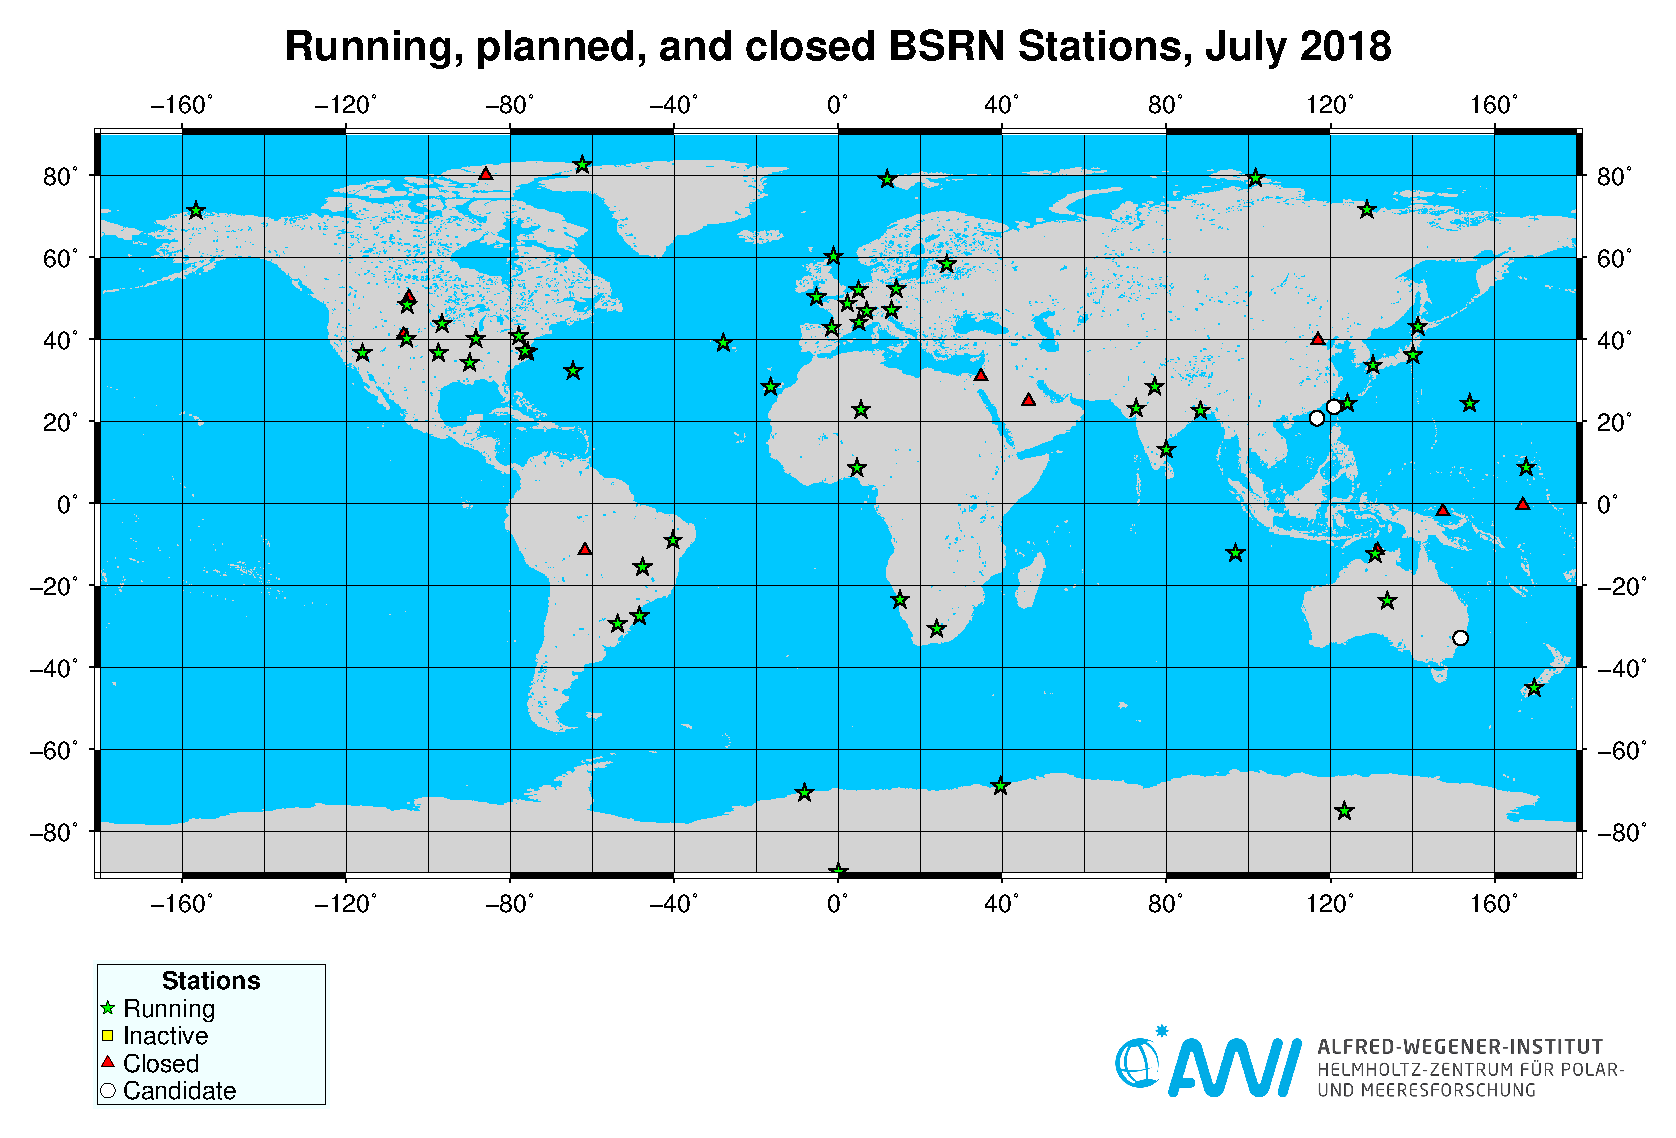
\includegraphics[width=0.8\textwidth]{DataMethodsFIGS/bsrn.pdf}
  \caption{Solar radiation stations from BSRN.}
 \label{fig:bsrnstations}
\end{figure}

\section{Modelling of solar radiation}

In order to understand the processes that take places when solar radiation goes through the atmosphere and reaches the Earth's surface it is necessary a modelling approach. This modelling process can be made by a physical approach or using statistical methods (Festa and Ratto, 1993).\\

The physical modeling of solar radiation is based on physical equations of the interaction between atmospheric components and solar radiation (aerosols, water vapour, clouds...). When solar radiation goes through the atmosphere, it can interact with its components being absorbed by molecules, backscattered to space or scattered in any other direction. Thus, only part of the solar radiation at the top of the atmosphere (TOA) will reach the Earth's surface.\\ 

This process is the physical process of energy transfer described by the radiative transfer equation (RTE) and its solution needs a radiative transfer model (RTM). The radiative transfer is a very complex process that needs to be simplified to be solved numerically and some parametrizations are needed. However, from these models it is possible to reproduce the solar radiation behaviour across the atmosphere and at the surface. RTMs are in the core of numerical weather prediction models and climate models and sometimes they are used to obtain solar radiation from satellite images, although in this case empirical or semi-empirical approaches are also commonly applied.\\

Secondly, the solar radiation at the surface can be estimated using statistical methods. In this case it is necessary to have enough data to validate the model and likely these models will not be able to reproduce solar behaviour universally. However, they can be very useful for local applications.\\

In chapters 6 and 7 different climate models are used as main source of solar radiation data. The output of each model will be the result of the radiative scheme inside their codes and it can be used as the input variable for a photovoltaic production model to analyse photovoltaic potential under different climate conditions.\\

\subsection{CORDEX initiative}

Under the acronim of CORDEX (Coordinated Regional Downscalling Experiment) there have been developed a wide range of regional climate models\footnote{The chapter \ref{cha:Methods} explain the origin of regional climate modelling and the simulations used in the thesis} that provide climate downscalled simulations for different areas around the globe\footnote{Cordex website:http://www.cordex.org/. This international framework is under the umbrella of the world climate research program, WRCP} . Their importance arise with the advance in knowdlege of climate change provided by global models. Whereas those models give an overview of the evolution of global conditions, their coarse resolution is not enough to understand climate change impacts at a local scale. The higher resolution of the regional climate models are needed for supporting adaptation and mitigation plans.\\

Two different domains from CORDEX are used in this study both focus on the Mediterranean area: EURO-CORDEX and MED-CORDEX (in figure \ref{fig:cordexdomain}). The horizontal resolution of the simulations included in EURO/MED-CORDEX go from 44º to 11º (from ~50km to ~12km).

\begin{figure}[!tbp]
  \centering
  \subfloat[Med-CORDEX]{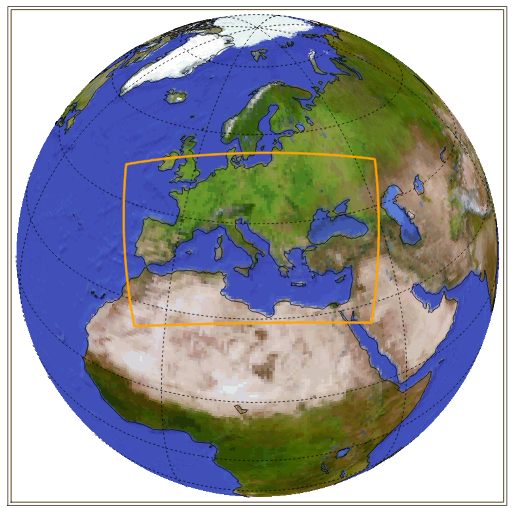
\includegraphics[width=0.4\textwidth]{DataMethodsFIGS/medcordex2}\label{fig:medcordex}}
  \hfill
  \subfloat[Euro-CORDEX]{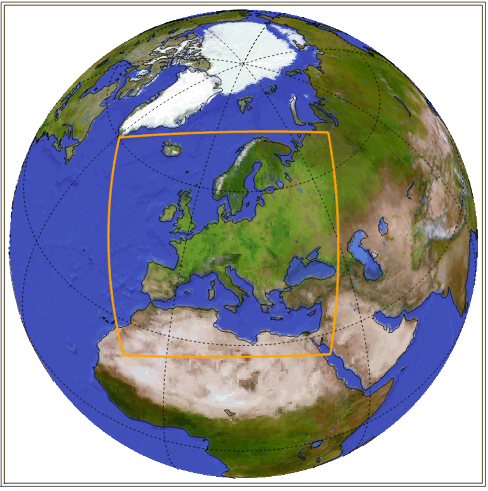
\includegraphics[width=0.4\textwidth]{DataMethodsFIGS/eurocordex2}\label{fig:eurocordex}}
  \caption{Domains from Med-CORDEX and Euro-CORDEX. Images from wRCP-CORDEX website.}
    \label{fig:cordexdomain}
\end{figure}

{\color{red}¿Incluir una tabla con los diferentes modelos regionales que participan en MED cordex y EURO cordex? Los que se usan en la tesis están explicados después, pero este es un punto general de dónde se han obtenido los datos.}
\section{Satellite data: \textit{Climate Monitoring Satellite Application Facility, CM-SAF}}

It has been previously commented that the scarcity of available ground-based solar radiation measurements is a well-known problem. Satellite datasets have become one of the main sources of solar radition data because of their high spatial and temporal resolution as well as their increasing accuracy.\\

There are different methods to retrieve solar radiation from satellite images that goes from physical models to empirical ones. In the first case, the models try to explain the radiance observed by the satellite instrumentation with a radiation transfer model (RTM). In order to do that, it is necessary to know the composition of the atmosphere. On the other hand, empirical models are based in simple regression models between the visible-channel's recorded intensity and grounded measurements. There are also some approaches that are in between theses two sides: the semi-empirical models. They use a simpler radiative-transfer scheme and some statistical regressions between data from satellite sensors and observed data (Schmetz (1989), Noia et al. (1993), Pinker et al. (1995), Zelenka (2001), and Hammer et al (2003)).\footnote{Jan Kleiss, Solar Energy Forecasting and Resource assessment, pp.22.23}\\

In this work some satellite-data-based products from CM-SAF (The Satellite Application Facility on Climate Monitoring) have been used. The aim of CM-SAF consortium from EUMETSAT [ref] is to develop satellite-data-based-products for climate monitoring since in 2000 it was recognised the importance of using satellite for this purpose.\\

The CM SAF products are derived from several instruments on-board operational satellites in geostationary and polar orbits. There are two main types of products that can be obtained from the CM-SAF: operational products and climate data records (CDR). The main purpose of the CDR is to provide a high-quality database to monitor climate variability and changes (ref), as well as the detection of trends. Operational products, on the other hand, are not accurate enough for this purpose because some errors like inter-satellite biases or sensors degradation are not corrected (ref: PUM producte user manual).\\


The SARAH dataset from CM-SAF has been used in chapters 6 and 7 of this manuscript for the analysis of shortwave solar radiation at the surface. The data is based on the records from Meteosat images, first and second generation, using the on-board MVIRI and SEVIRI instruments respectively. As the purpose of the CDR is to provide long time series convering more than 20 years, it is necessary a retrieval algorithm that can be applied to SEVIRI intruments as well as to the older MVIRI. This algorithm has been called MAGICSOL and has to parts: first, the modified Heliosat method is used to obtain the cloud effective albedo (CAL) and second, the MAGIC appoach is used to obtain all sky surface radiation based on CAL. (ref PUM)\\

{\color{red} No sé si merece la pena poner algo más acerca del método. Puede ser de ayuda también para ver como se incluyen los aerosoles. Incluyo una imagen del esquema que hice del proceso de obtención de la radiación con los datos del satélite y podría estar bien incluir.}\\


\begin{figure}
  \centering
  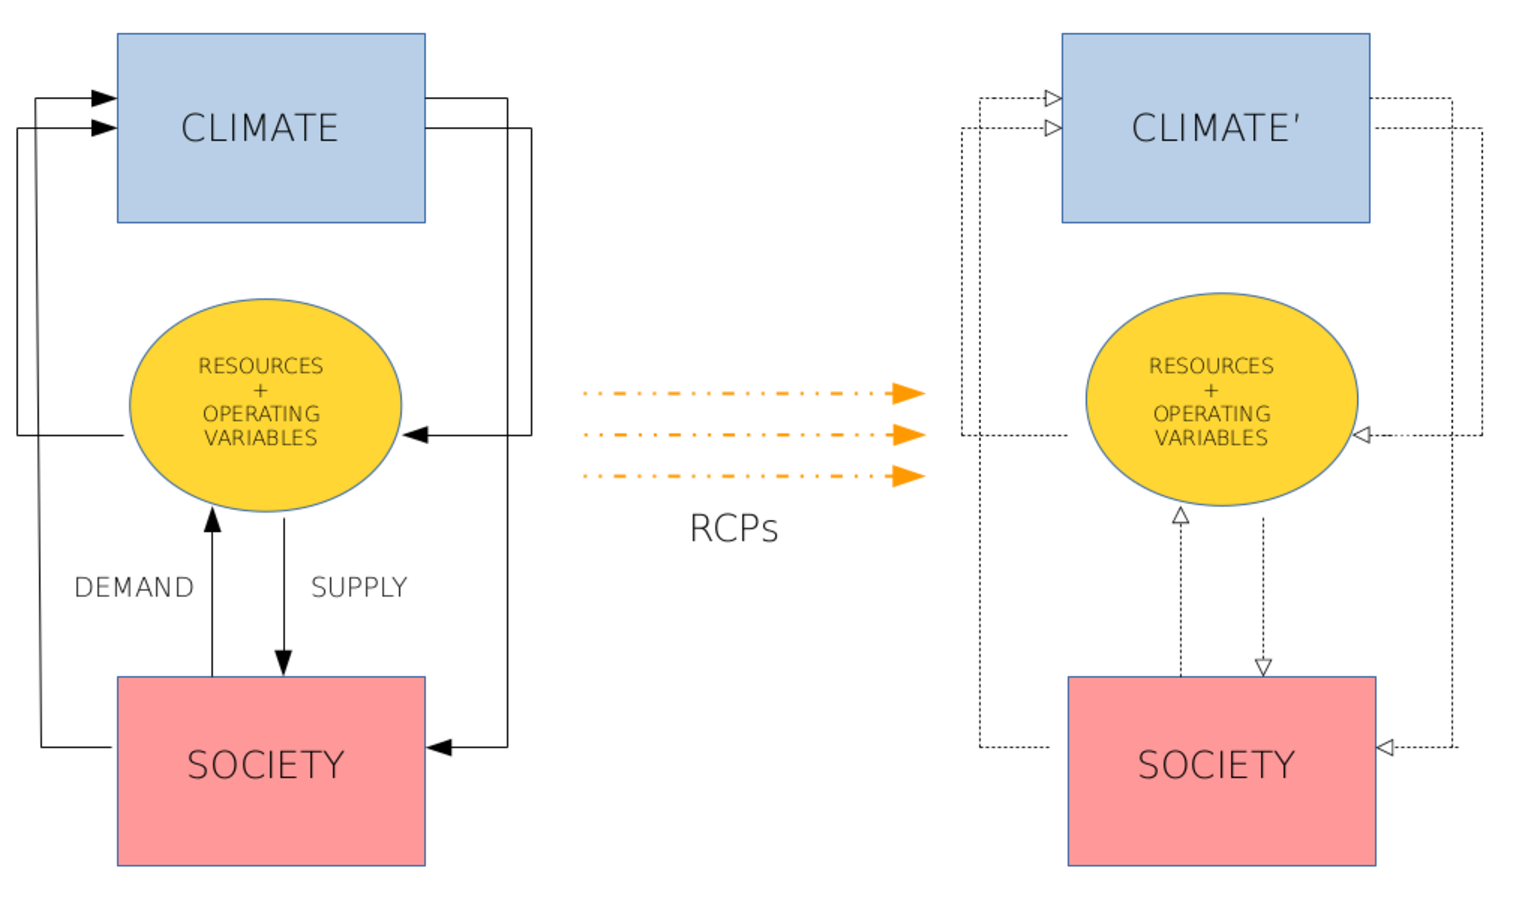
\includegraphics[width=0.6\textwidth]{figs/esquema}
  \caption{Algorithm scheme: Retrieval of shortwave solar radiation from satellite images.}
 \label{fig:algorithm}
\end{figure}

\section{Photovoltaic prodution data}

In order to evaulate the performance of a PV model it is necessary to use the data from real PV plants. However, these data is not easy to obtain, due to the fact that it belongs to private companies and it could compromise some of their strategies. This makes necessary to get agreements and confidential contracts between these companies and researchers that are not always easy to obtain if an inmediate benefit does not arise from those relationships.\\

Some alternatives are the databases of aggregated data that are available for the European countries throught the ETNSO-e data portal website. However, these data will be only useful for certain modeling exercices.\\

\begin{itemize}
\item {\color{red} ¿Tiene sentido que comente aquí los datos de ETNSO?}
\item {\color{red}No tengo claro si describir aquí las dos plantas que tenemos y que se utilizan en el segundo artículo}\\
\end{itemize}

\section{Temperature data}

  In adittion to the direct relationship between solar irradiation and photovoltaic energy conversion, there are other atmospheric variables that influence the performance of solar cells, like temperatura or wind speed. The model used in this work consider only temperature as a second order factor that reduces cell efficiency as it is explained in chapter 4.\\
 
  Temperature data is easier to obtain than solar radiation data. Numerous weather stations provides temperature data at 2m over the surface at a local scale. For an overview of a large area gridded products are useful and easier to combine with the satellite products.\\

  E-OBS is a gridded dataset derived through interpolation from the ECA\&D data based on stations that provides daily temperatura data over Europe and the Mediterranean area \footnote{https://www.ecad.eu//download/ensembles/download.php#maps}. This product has been validated in several research papers (Begert et al. 2008, Hofstra et al. 2009a,b) finding that some inaccuaracies related to an over-smooth exists in areas where there are few stations, which affects mostly to the extreme analyses.

{\color{red} ¿Quizás incluir aquí un mapa con las estaciones a partir de las que se hace la interpolación}  
%%%%%%%%%%%%%%%%%%%%%%%%%%%%%%%%%%%%%%%%%%%%%%%%%%%%%
\chapter{Methods\label{cha:methods}}

In order to fullfill the objectives of the present work it is necessary to apply different methodologies in each of the results chapters, all of them has been explained in detail at the corresponding section.\\ %In general, they goes through the statistic analysis of different variables related to solar resource and photovoltaic production, where the latter comes from an estimation using a PV model. %The analysis is also developed in different time scales, which leads to the necessity of adapt the same methodology to each case.\\

However, in the present chapter the different tools needed for the development of each study are described in a general manner. The three results chapters are based in a \textbf{modeling chain} that includes a photovoltaic model that is composed of two basic steps. First, the transposition to the plane-of-the-array, POA, of the components of the solar radiation, which implies also to assume some simple models of the atmosphere sphere seen from the generator plane and a model for the electrical performance of the system. Besides, the input of this PV model can be solar radiation measurments, satellite radition estimations o, as we saw in the previous chapter, the output of atmospheric/climate models. \\

%En general, el método consite en la creación de una cadena de modelado que incluye un modelo de producción fotovoltaica, compuesto por el paso al plano del generador fotovoltaico de las componentes de la radiación solar y un modelo de funcionamiento eléctrico del sistema. Además, se el input de este modelo fotovoltaico podrán ser observaciones de radiación solar medidas en superficie, estimaciones de satélite o, como vimos en el capítulo anterior, radiación solar obtenida a partir de la salida de modelos.
%  En el primer capítulo, se analizará de manera espacial la variabilidad interanual y la complementariedad del recurso solar en la Península Ibérica, para lo que se aplicarán técnicas de \textbf{clustering}. La evaluación de la productividad fotovoltaica lleva asociada la necesidad de la \textbf{modelización de un sistema fotovoltaico}.\\

  In chapter 5 it is analysed the interannual variability and complementarity of solar resource over the Iberian Peninsula and for that purpose we apply \textbf{clustering techniques}. The regionalization allow us to simplify the spatio-temporal analysis of solar resource. The evaluation of the productivity, defined as the amount of energy produced by a PV system normalized by the power capacity of the system, means the \textbf{modelization of the photovoltaic system}.\\
  
  The chapter 6 analyses the impact of \textbf{aerosols} in photovoltaic productivity over the Euro-Mediterranean area.  Some climate simulations are used as the input of the photovoltaic model. The modelling chain allows to make a sensitivity test to quantify the role of aerosols in the area.\\

%  En el segundo capítulo se estudia el impacto de los aerosoles en la producitvidad fotovoltaica, esta vez en el área Euro-Mediterránea. En este caso, las \textbf{simulaciones climáticas} serán utilizadas como input del modelo fotovoltaico, creando una cadena de modelado que permita realizar un ejercicio comparativo de sensibilidad para cuantificar el papel de los aerosoles.\\
  
  Finally, the photovoltaic energy potential is analysed in the future, using \textbf{climate projections} from different climate models. Trends and anomalies with respect to a reference period are evaluated. In this case, a \textbf{multi-model analysis} through different RCMs simulations allow us to evaluate the solar resource under climate change scenarios. The representation of aerosols in the climate projections is consider as a fundamental variable for the shortwave downward radiation projections, SSR, and PV productivity.\\ 

%  Por último, se realiza el análisis del potencial fotovoltaico futuro, evaluando las tendencias y anomalías con respecto a un periodo de referencia. En este caso, se hace un \textbf{estudio multimodelo} a través de distintas simulaciones de diferentes RCMs que permita evaluar el recurso solar y se utilizan las mismas para el cálculo de la producción fotovoltaica. En este último punto vuelve a considerarse la representación del campo de AOD dentro de las simulaciones climáticas como variable determinante en las proyecciones de SSR y productividad PV.\\
  
\section{Clustering algorithm applied to climate data}
% The culstering algorithms are design for grouping together variables and recognise patterns between them that are difficult to see at first sigth. This algorithm were first applied in ... and they have grown quickly adapting to a highly data-driven world.

% Pattern recognition: extraer objetos y agruparlos en clases. Dependiendo de las distintas disciplinas, estos objetos pueden ser muy diferentes. Se utiliza el pattern recognition en el reconocimeiento de imágenes, de palábras, ayuda en el diagnóstico, o para el análisis de bases de datos en data mining. En este último, las aplicaciones van desde la biología a las finanzas o ciencias sociales y en un data-driven world, cada vez adquiere una importancia mayor, transformando los datos en conocimiento.

% En primer lugar, se definen las características que se van a emplear como medida de similitud/similaridad utilizada para la clasificación. Una vez que estas características están definidas, los algoritmos de clustering se encargan de agrupar  estas características.

%En un mundo cada vez más movido por los datos, el reconocimiento de patrones se ha utilizado en  muchas disciplinas, desde la biología a las finanzas o las ciencias socialses, para extraer información relevante de los diferentes conjuntos de datos. Éstas técnicas, ayudan a conocer relaciones difíciles de extraer a simple vista, bien por el volumen de los datos, o por la complejidad de las mismas y la cantidad de variables involucradas. 

In a data-driven world, \textbf{pattern recognition} is being applied to many disciplines from biology to finanze through social science, in order to obtain relevant information from different datasets.
However, if the similarity measurements can not be define first, due to unknown previous labeled data, another approach will be implemented. In that case, the task will consist in identifying the similarities afterwards, from a dataset of features, applying clustering algorithms for that purpose.

\subsection{Clustering algorithms}

It is not under the scope of this work to analayse in detail all the clustering methods available, due to the vast number of them and its increasing complexity [ref:data clusterng a review]. However, it is worth it to give an overview of its classification and application in order to better understand the choice made in the study of our problem.\\

There are different types of clustering algorithms based on its application and the criteria applied to construct the clusters. The two main categories are divided in \textbf{hierarchical} and \textbf{non-hierarchical algorithms}, but there are other taxonomies based on the algorithm construction that can be used to classified different methods [ref].\\

The \textbf{hierarchical clustering algorithms} create a number of nested clusters and they can be also divided themselves in agglomerative or divisive. The first one, obtain a smaller number of cluster in each step, whereas the divisive algorithms work on the other direction.\\

Most of these hierarchical algorithms are variants of the single-link or complete-link algorithms. They have a different way to measure similarity. In the first case, the distance between two clusters is the minimum of all the pairwise distances measured between the objects of the two clusters, in contrast, for the complete-link algorithm the distance is considered the maximum of all the pairwise distances.\\

On the orther hand, the non-hierarchical or \textbf{partitional clustering algoritm}, create a number of non-overlapping clusters. These methods could be useful when the amount of data involved is large and the construction of a dendogram, produced by the hierarchical algorithm could be computational expensive.\\

The partitional methods create the group of clusters using an \textbf{optimization function} which defines the similarity. The main inconvenient of these algorithms is the in-advanced definition of the number of clusters. Usually, the algorithm is implemented several times for a wide number of partitions and the optimum number of clusters is defined afterwards using validity index criteria.\\

%{\color{red}{Añadir algo más sobre algoritmos partitional}}


\subsection{Clustering climate data}

As previously commented, the use of pattern recognition and in particular, the clustering analysis, has been widely used across many different disciplines. The use of these techniques to group together atmospheric variables that could help in environmental classifications is a more recent research field.[ref]\\

Historically, the climatic divisions were based mostly on the differences in vegetation types around the globe. The Koppen-Terawata classification [ref] is the most widely known climate classification and bases its divisions in obtaining the vegetation thresholds from precipitation and temperature data. Some authors had already pointed the limitations of this classification method mostly due to two aspects: the first one is that vegetation thresholds are not well defined and that could be an issue when higher spatial resoultion scales want to be defined. On the other hand is the fact that not only precipitation and temperature are influencing the vegetation species but also other atmospheric variables like solar irradiation, as well as other environmental factors that could be related to antropoghenic emissions or waste.\\

%{\color{red}{Buscar más biblio de esto}}

As these classical division are not adapted to the necessities of different fields and could be even biased, another way to geo-spatial classification is needed. In this sense it has become frequent to sucessfully use data-driven classification of different variables if it is necessary to give an spatially resolved answer. [ref]

\subsection{Applied clustering method}

In this work a clustering method is applied to classify solar irradiation due to the fact that classical climate divisions are only based on temperature an precipitation. The spatial pattern tha could be extract from the Koppen-Terawatta classification, can not be used for our pourpose.\\

A partitional commonly used clustering method has been selected to classify solar irradiation of the area. The \textbf{'k-means'} algorithm is easy to implement, due to the fact tha has been largely used over the literature. Moreover, the combination of a \textbf{principal component analysis} of the dataset previous to the k-means algorithm application has been proved to be an useful tool to reduce the data-dimensionality and apply the algorithm in a more efficient manner.[ref]

\subsubsection{K-Means algorithm}

The k-means algorithm is a partitional clustering method that provide a set of partitions from the application of an optimization function, usually the euclidean distance, \ref{eq:euclidean}. The algorithm initiates from a pre-defined number of clusters, 'k', and randomly selects a group of centroids equal to the number of clusters. The optimization function is applied to assign each object to one of the clusters, depending on the similarity (distance) to each of the centroids. This proccess is applied until the algorithm converges.\\

\begin{equation}\label{eq:euclidean}
    J =\sum_{i=1}^{k}\sum_{j=1}^{n}{||x_i-c_j||}^2
\end{equation}

One of the limitations of these method is its dependency on the first selection of the centroids, that could lead to a local optimum instead to a global optimum. To solve this difficulty, the algorithm can be run many times to test the sensitivity of the algorithm to a different initial conditions. Another option is to use an initialization technique to select the centroids.\\

As the number of clusters 'k' is not normally known in advance, the algorithm is applied from 2 to 'n' times, with 'n' high enough to get the whole variability of the dataset and the optimum number of clusters is defined afterwards. This optimum 'k' will define the number of clusters that explain most of the variability and will assure that the increase in the number of clusters does not improve the variance representation. [ref]\\

\subsubsection{Principal Component Analysis}

The Principal Component Analysis, PCA [ref], consists in a decomposition of the dataset into a number of vectors whose linear combination represents the original data. The transformation of the original data into a lower dimensional space is a reduction of the dimensionality retaining the maximum of the data variance.\\

The new orthogonal system has in its first coordinate axis, the projected values of the original data that preserve most of the variance in the dataset, and it is called the principal component. The rest of principal components decrease the amount of variance explained consecutively.\\

The PCA has been applied in advance to K-means clustering algorithm among the literature [ref]. It was explained by [ref] that the reduction in dimensionality is directly linked to K-means due to the fact that the clustering membership indicators are actually the eigenvectors given by the PCA. For this reason, it has been applied before the K-means algorithm fastening the algorithm.\\

\subsubsection{Validity Index}

Clustering validation through the validation or validity index measures the goodness of the clustering results. As well as the clustering techniques, there is a classification for the methods used to validate the clustering results.\\

External validation techniques use information outside the dataset involved, whereas the internal validation techniques only need the information that is present in the data. The external methods knows the number of optimal clusters in advance, so they are applied to select the best clustering algorithm. On the other hand, the internal validation methods will give us the optimum number of clusters after the application of the selected algorithm and only use the information that rely on the data.\\

Two different index are used in this study, the \textbf{Calinski-Harabasz}\footnote{In the equation \ref{eq:calinski}: The 'BCSM' is the Between-Cluster-Scatter-Matrix, and its trace is the sum of squares distances between each cluster center $c_{i}$ and the global centroid vector of all the objects of the dataset. The term 'WCSM' is the Within-Cluster-Scatter-Matrix and the trace of this matrix is the sum of squares of the distances between the objects inside each cluster and the centroid. 'k' is the number of clusters} index (Eq.:\ref{eq:calinski}), the \textbf{Davies-Bouldien}\footnote{In the equation \ref{eq:davies}: $d_{i}$ is the averaged distance between the data clasiffied to class i and the clauster center $c_{i}$ and $d(c_i,c_j)$ is the distance between the different cluster centers. 'k' is the number of clusters.}  index (Eq.:\ref{eq:davies}), and the L-method proposed by Salvador and Chan, 2005 [ref]. Similar results are obtained with them. In order to analyse the optimum partiton, is important to consider the nature of the variables that we are analysing. Most of the atmospheric variables, are continious variables that could be closely related to other variables such as latitude. For that reason, the regionalization procedure can not be applied like for other discrete or non-continuous data. That characteristics should be considerd when the results have to be evaluated.\\

\begin{equation}\label{eq:calinski}
    CH =\frac{trace_{BCSM}}{trace_{WCSM}}\times\frac{n-k}{k-1}
\end{equation}

\begin{equation}\label{eq:davies}
    DB =\frac{1}{k}\sum_{i-1}^{k}\max_{i=1,...i\neq{j}}{\frac{d_{i}+d_{j}}{d(c_i,c_j)}}
\end{equation}

%\subsubsection{Initialize K-Means}
\section{Simulating a photovoltaic system}

The process of simulating a photovoltaic system has two main steps. First, it is necessary to estimate the amount of energy that reaches solar cells to be transformed into electricity. This energy will be defined as \textbf{global effective irradiation}, $G_{eff}(\alpha, \beta)$. Secondly, the amount of energy that the system is able to give depends on the electrical performance of its components, which is the second part of the modeling process.\\

Both stages involve some modeling assumptions and each one would be explained in detail in the following sections. In general, due to the fact that it is very unlikely to obtain solar radiation measurements in the plane-of-array ($G(\alpha, \beta)$), global horizontal irradiation ($G(0)$) (the most common variable measured or modeled that can be obtain from different sources), will be the starting point. In order to estimate the amount of energy that reaches the generator surface, $G(\alpha, \beta)$, it is necessary to do a transposition of the different radiation components from the horizontal plane $G(0)$ to the plane of the array (POA).\\

Once the solar irradiation components at the generator surface are calculated, it will be assessed how much of that energy can be transformed into electricity. The relative position between the generator and the sun gives the optical losses according to the difference with the optimum incident angle. After considering the optical losses the plane of array irradiation becomes the global effective irradiation $G_{eff}(\alpha, \beta)$.\\
% In order to estimate the amount of energy produced by a photovoltaic system it is necessary first to assess the amount of energy that reach the generator surface (plane of array irradiation, $G(\alpha, \beta)$) and after this estimation, which it is not straightforward unless it is measured, the different components of the generator has to be modeled.\\

The second step that will calculate the energy output will indicate the performance of the electrical components from the global effective irradiation and other variables that can influence on cells, like ambiance temperature. The whole photovoltaic system includes the generator, the inverter and the transmission elements and wires.\\

% For the evaluation of the photovoltaic \textbf{energy yield}, defined as the amount of energy produced by a photovoltaic system divided by its nominal power, along this work we use the process explained below, which can be summarized in two steps:

% \begin{enumerate}
% \item To calculate the \textbf{effective irradiation}, $G_{eff}(\alpha, \beta)$, which is the effective irradiation after substract optical losses, due to reflection, angle of incidence or dirtiness. The assessment of this variable has to be done from the global irradiation at the surface, $G(0)$, that can be obtain from measurements, atmospheric models or satellite datasets.
% \item The second step consists in simulate the \textbf{electrical performace} of the system and estimate the power from the generator. The whole photovoltaic system includes the generator, the inverter and the transmission elements and wires.
% \end{enumerate}

All the processes involved in the stage of simulating a photovoltaic system in this thesis have been made using solaR [ref], an R package that implements all the necessary functions to estimate the energy provided by the system.

\subsection{Global effective irradiation}

Assessing the amount of energy reaching cells of the photovoltaic generator requires to compute trackers movements, as well as the relative position between sun and panels throughout the year, a detailed description of these methods can be found in \citep{Perpinan.Marcos.ea2013}.  Once these equations are computed, the procedure is described below:\\

First, global irradiation on the horizontal plane is decomposed in two components, \textbf{direct} and \textbf{diffuse} irradiation, Eq.\ref{GlobalIrradiation}. The third component of global irradiaiton, the albedo, it is  not consider because its contribution is very low. To estimate these quantities we will consider equations proposed by \cite{Liu1960} to characterize solar irradiation. Definition of \textit{clearness index}, Eq.\ref{K.indicedeclaridad}, is the ratio between global irradiation and extra-terrestrial irradiation at the horizontal plane. They also proposed to relate that index with the \textit{diffuse fraction}: the ratio of diffuse to global irradiation in Eq.\ref{F.diffusefraction}. This relation varies depending on the time scale. For daily values, we estimate correlation between the clearness index and the diffuse fraction using equations in \cite{Aguiar1992}. After that, the diffuse component is obtained with the definition of the \textit{diffuse fraction}, Eq.\ref{F.diffusefraction}.

\begin{equation}\label{GlobalIrradiation}
G_{d}(0) = B_{d}(0) + D_{d}(0)
\end{equation}

\nomenclature[G]{$G(0)$}{Global irradiance on the horizontal plane.}
\nomenclature[Gd]{$G_{d}(0)$}{Daily global irradiation on the horizontal plane.}
\nomenclature[D]{$D(0)$}{Diffuse irradiance on the horizontal plane.}
\nomenclature[Dd]{$D_{d}(0)$}{Daily diffuse irradiation on the horizontal plane.}
\nomenclature[B]{$B(0)$}{Direct (beam) irradiance on the horizontal plane.}
\nomenclature[Bd]{$B_{d}(0)$}{Daily direct (beam) irradiation on the horizontal plane.}


\begin{equation}\label{F.diffusefraction}
F_{D,d}=\frac{D_{d}(0)}{G_{d}(0)}
\end{equation}

\begin{equation}\label{K.indicedeclaridad}
K_{Td}=\frac{G_d(0)}{B_{0d}(0)}
\end{equation}

Secondly, daily irradiance has to be estimated from irradiation values. Considering low variability of solar irradiance, it is assumed that average irradiance in a short interval coincides with irradiation in that interval. Regarding equations proposed by \cite{Aguiar1992}, the ratio of the diffuse irradiance to diffuse irradiation is assumed to be equivalent to the ratio of extraterrestrial irradiance to extraterrestrial irradiation Eq.\ref{ratioB0}, and the ratio of global irradiance to daily global irradiation is followed from the same reference Eq.\ref{ratioG0}. 

\begin{equation}\label{ratioB0}
r_{D}=\frac{D(0)}{D_d(0)}=\frac{B_0(0)}{B_{0d}(0)}
\end{equation}


\begin{equation}\label{ratioG0}
r_G=\frac{G(0)}{G_d(0)}=r_D\cdot(a+b\cdot\cos(\omega))
\end{equation}

\nomenclature[Ktd]{$K_{Td}$}{Clearness index.}
\nomenclature[Fd]{$F_{D,d}$}{Diffuse fraction.}
\nomenclature[B0]{$B_0(0)$}{Direct (beam) extra-terrestrial irradiation.}
\nomenclature[B0d]{$B_{0d}(0)$}{Daily direct (beam) irradiation.}

The third step considers only geometrical criteria to compute the direct and diffuse irradiance components at the inclined plane. Diffuse irradiance is calculated with the anisotropic model proposed in \cite{hay1985estimating}.\\ 

The last step estimates the effective irradiance incident on a generator subtracting dust and angle of incidence losses from the incident irradiance with the model proposed in \cite{Martin2001}.\\

In figure \ref{fig:algorithm_outline} the steps to assess effective irradiation at the plane-of-array is summarized.

\begin{figure}
  \centering
  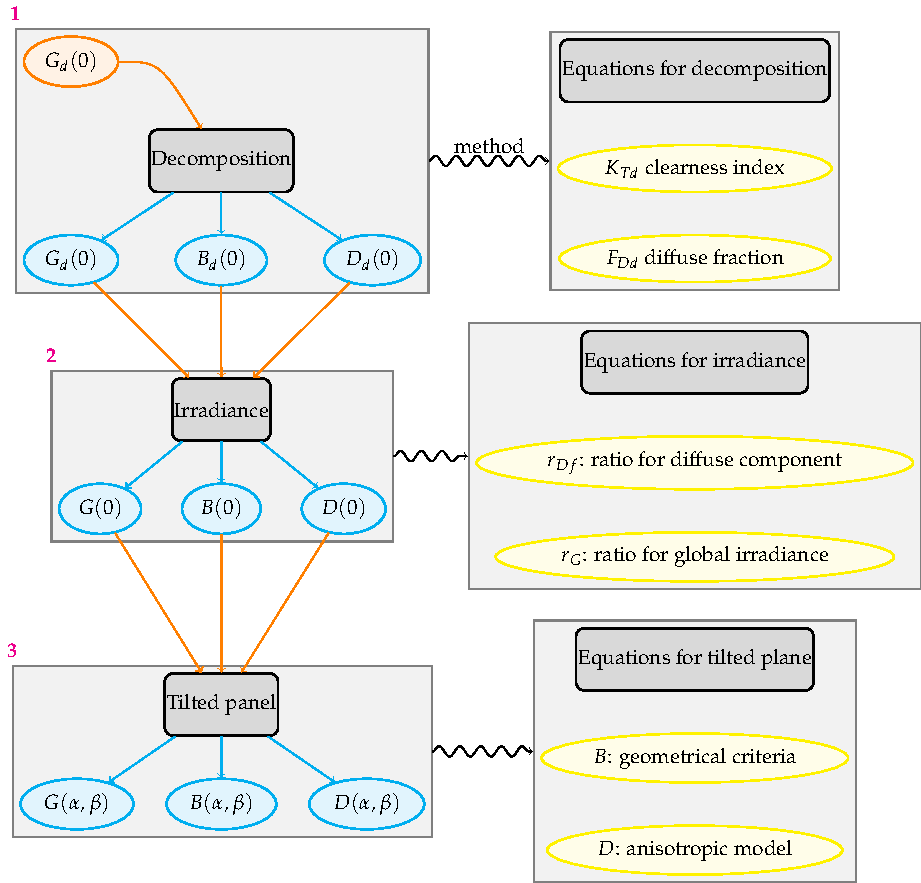
\includegraphics[width=0.6\textwidth]{figs/algorithm_outline}
  \caption{Algorithm scheme: steps on the calculation of incident irradiation at the inclined plane. Orange color means input of the calculation and blue color output or results. If a result in a previous step is used in the next one, arrows linking steps are orange. Right side of the scheme represents the method and equations needed.}
 \label{fig:algorithm_outline}
\end{figure}

\subsection{Photovoltaic energy yield}

Once the effective irradiation that reaches solar cells is being assessed, the transformation into power output depends on some factors regarding the photovoltaic system. In order to estimate  potential for photovoltaic production, the term ``yield'' is defined as the energy produced by the power installed $[\si{\kilo\watthour\per\kilo\wattpeak}]$. That energy, comes from the integration in each time step of the power output of the photovoltaic system.\\

Considering that a photovoltaic generator is composed of modules, the generator nominal power output is calculated by multiplying the power output of a single module by the number of them, assuming the same electric performance of all modules. \\

\begin{equation}\label{Pout}
P_{out}=I_{m} \cdot V_{m}
\end{equation}

\nomenclature[P_out]{$P_{out}$}{Power output from the photovoltaic module}
\nomenclature[Im]{$I_m$}{Intensity from the photovoltaic module}
\nomenclature[Vm]{$V_m$}{Voltage of a photovoltaic module}

Ambient temperature influence cells performance. The assumption used to this assessment consider a linear relationship between cell temperature and global effective irradiation, Eq.\ref{Tcelula}. NOCT in equation \ref{Tcelula} is considered constant being the temperature of a cell when it works in determined conditions: irradiance of 800 $[\si{\watt\over\metro^2}]$ and ambient temperature of $20ºC$.

\begin{equation}\label{Tcelula}
T_c=T_a + G_{ef} \cdot \frac{NOCT-20}{800}
\end{equation}

\nomenclature[T_c]{$T_c$}{Cell temperature}
\nomenclature[T_a]{$T_a$}{Ambient temperature}
\nomenclature[G_ef]{$G_{ef}$}{Global effective irradiation}

After considering all these factors, the power output of the whole system is assessed by the consideration of a common inverter for transforming DC current into AC, also arrangement losses of the generator are included. Other systems factors that influence the performance of the photovoltaic system are shadows over the generator due to the positions of the PV modules over the land. This factor is not consider in our calculations assuming that we look for an estimation of the potential yield of an area, not the product of a real PV plant. Detailed description of the software employed to the assessment, solaR, is in \cite{Lamigueiro2012}. The process for the photovoltaic output is summarized in table \ref{tabla1} including all the steps and elements involved as explained in \cite{Perpinan2009}.

\begin{table} 
  \begin{tabular}{>{\raggedright}m{6cm}>{\raggedright}m{6cm}}
    \toprule 
    Element & Method\tabularnewline
    \midrule
    PV generator & Identical modules with
    $dV_{oc}/dT_{c}=0,475\frac{\%}{\celsius}$ and $NOCT=47\celsius$. 
    The MPP point calculated as in \cite{garcia2005caracterizacion}). \tabularnewline
    \midrule
    Inverter & Efficiency equation proposed in
    \cite{jantsch1992results}:  
    \begin{equation}
      \eta_{inv}=\frac{p_{o}}{p_{o}+k_{0}^{o}+k_{1}^{o}p_{o}+k_{2}^{o}p_{o}^{2}}
    \end{equation}
    where $p_{o}=P_{ac}/P_{inv}$ is the normalized output power of the inverter. The characteristic coefficients of the
    inverters are: $k_{0}^{o}=0.01$, $k_{1}^{o}=0.025$, $k_{2}^{o}=0.05$.\tabularnewline
    \midrule
    Other losses & \begin{itemize}
    \item Average tolerance of the set of modules, $3\%$.
    \item Module parameter dispersion losses, $2\%$.
    \item Joule losses due to the wiring, $1.5\%$.
    \item Average error of the MPP algorithm of the inverter, $1\%$.
    \item Losses due to the MV transformer, $1\%$.
    \item Losses due to stops of the system, $0.5\%$.
    \end{itemize}
    \tabularnewline
    \bottomrule
  \end{tabular}
  \caption{Calculation procedure for the estimation of energy produced by a PV
    system from daily global horizontal irradiation data. Left column represents the element of the PV system and the right column the equations and methods used in each case for the efficiency of the elements.}
  \label{tabla1}
\end{table}

\nomenclature[Pinv]{$P_{inv}$}{Nominal
  power of the inverter}
\nomenclature[po]{$p_{o}$}{Normalized output power of a inverter}
\nomenclature[kinv]{$k_{i}^{o}$}{Coefficients of the
  efficiency curve of a inverter}


\section{Using Regional Climate Models}

%La cadena de modelado necesaria para obtener una estimación de la producción fotovoltaica puede incrementarse introduciendo como input una estimación o una salida de otro modelo (meteorológico, climático...) en lugar de observaciones. Este paso aumentará la incertiumbre de la potencia entregada por el sistema, pero merece la pena tomarla en consideración teniendo en cuenta la escasez de estaciones de medida que proporcionan datos de radiación.\\
The modeling chain to obtain an estimation of the photovoltaic production of a system starts with the input of the PV model. We can consider the output of an atmospheric or climate model as the input of the PV system instead of solar radiation measurements. The uncertainity of the PV power output will increase but it is worth it to consider this option because of the lack of reliable and well spread station measurements.\\  
 
%En nuestro contexto, en el cual la longitud de las series temporales es clave\footnote{el estudio climático es la evaluación del comportamiento medio de las distintas variables a lo largo del tiempo, su variabilidad y tendencias. Para poder definir una climatología se considera en consenso que son necesarios 30 años da datos.}, los modelos climáticos son una herramienta que permite evaluar el recurso presente, su evolución futura así como server de input en la cadena de modelado para estimar la potencia entregada por un sistema fotovotaico.\\  

In our context, with the purpose of analysing solar radiation and the potential PV production form a climatological point of view, climate models are a good tool that allow us to evaluate the resource in present conditions as well as its future evolution.\\

The history of climate modeling has been linked to the computational development since its beginning. The mathematical representation of the climate system was a consequence of the advance in numerical weather prediction models that took place for the first time in Princeton in 1952 and that had a fast grow. [ref and {\color{red}develop a bit more?}].\\

Climate modeling is based on a 3-D representation of the whole climatic system, where the Earth is divided  in a 3-D spatial grid whose size or resolution has evolved in time with computational power. Equations of motion, momentum and conservation laws are solved for each gridbox. As some of the atmospheric processes occurs in a finer spatial scale than the resolution of the model, parametrizations are needed for some processes such as convection. These models were first named as General Circulation Models, GCM, as their aimed was to represent main circulation flows in the atmosphere, but the development of more complex models that would start to include ocean and land, would name later these models as \textbf{Global Climate Models, GCMs}. \\

Since its origins, there has been a diversification and more research groups has developed its own climate models. Also, many international framework initiatives has unify efforts to understand better the future evolution of climate with the intensification and promotion of research collaboration programs that include all the models (WCRP, IPCC, CLIVAR...)\\   
%``L. F. RichardsonZ was the first to promote the idea that future weather could be predicted by numerically integrating the equations of fluid motion using the present weather as the initial condition.  The first successful numerical forecasts used a  set of equations that are greatly simplified compared to Richardson’s and for which the solution is less sensitive to the initial conditions.''

Global climate models provides reliable information about the possible evolution of climate in large scales. Their horizontal resolution, however, covers areas with very different regional characteristics, which potentially miss some information that affect in a particular manner to smaller and vulnerable areas.\\

It was in the early 90s (Dickinson 1989 and Giorgi 1990) when it was proposed to use global models as the necessary boundary conditions to force a 'limited area model LAM'. Those LAMs had been used for numerical weather prediction forecast, but they were applied to predict the weather just few days in advance. The idea of run these simultaions for longer periods will result in the evolution of \textbf{Regional Climate Modeling}, what would provide regional climate information of processes that occurs in a spatial scale not resolved by a global models.\\

In a similar way than the GCMs, RCMs community has expanded in last decades and the number of research groups has increased. Also, some international initiatives try to engage different groups and modellers to develop better models and simulations (PRUDENCE, ENSEMBLES,CORDEX, EURO-CORDEX, MED-CORDEX).\\

In the present work we make use of RCMs focused on the Mediterranean area, considering the models and simulations included in the EURO-CORDEX and MED-CORDEX projects.\\

These RCMs can provide the necessary atmospheric variables for the analysis of renewable energy resources. Due to its complexity and the need of parametrizations for some atmospheric processes, they can have sistematic bias that make difficult to use them for resource assessment. However, due to the low frequency variability observed in some variables and to the importance of considering the future projections, they are a valuable tool for analysing renewable energy resources and its evolution. Besides, the use of climate models allows to study specific climatic events and to understand its mechanisms, linking the implications of those situations with renewable generation.\\

For chapter 6, ``Impact of aerosols in photovoltaic energy production'', only one RCMs is used. Three different simulations are used in this chapter in order to quantify the sensitivity of PV energy production to changes in atmospheric aerosols content. The simulations are centered in the Mediterranean area, with the domain described by the MED-CORDEX initiative. The simulations length and characteristics of the aerosols dataset included are explained in detailed in the corresponding chapter.\\


% \begin{figure}
%   \centering
%   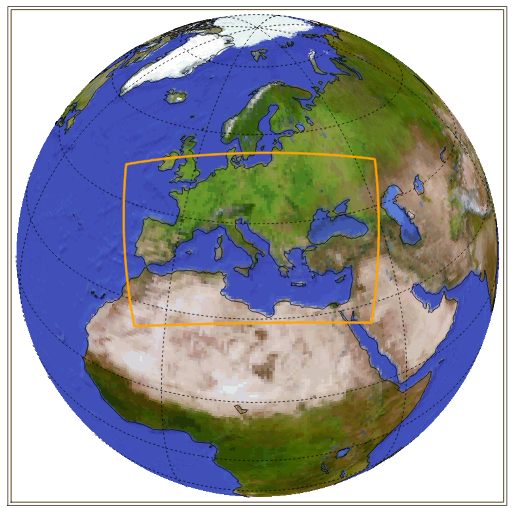
\includegraphics[width=0.4\textwidth]{DataMethodsFIGS/medcordex2}
%   \caption{Med-CORDEX domain}
%  \label{fig:medcordex}
% \end{figure}

\section{Future projections and scenarios}

Behind the comprehensive study of the climate system it is not only the interest of a deeper understanding of the physics processes but also there is a concern about the impact that a changing climatic system could have in the ecosystems and different species of the Earth.\\ 

The Intergovernmental Panel on Climate Change, IPCC, was launched in 1992 and it is an international organism that was founded by the World Meteorological Asociation, WMO, and the United Nations Environmental Program, UNEP. Its purpose was to gather together all the scientific information available about the anthropogenic climate change. This information will summarize our knowdlege about climate change, its impacts as well as some mitigation strategies were elaborated.\\

In order to elaborate the climate scenarios, which means the possible evolution of the climate system based on the actual climate conditions and models, it is necessary also to generate different plaussible scenarios of emissions. The development of these emission scenarios of greenhouse gases or aerosols will be based on the assumptions about technological changes or demographic criterias as well as the socioeconomic development of each region. Those scenarios, with different options for the future evolution, will be the driving force for the climate simulations in order to elaborate the climate projections.\\

The first emission scenarios were elaborated in the 90s and they have changed since then. For the 5th AR of the IPCC, that was released 2014 were defined the RCP scenarios. They are different 'representative concentrations pathaways' that correspond to the one of the possible scenarios that leads to an specific radiative forcing, i.e, the RCP8.5 represents a radiative forcing of 8.5 $[\si{\watt\per\metro^2}]$\\

For chapter 7, ``Future projections for PV technology'', several RCMs and its correspondin GCMs are used. The simulations include the historical period and the future scenario RCP8.5 or RCP4.5. The analysis of the results will be done with respect to a reference historical period.\\

In table \ref{climatemodels} there is a summary of the climate models and the simulations that are used in chapter 6 and 7.\\

\begin{table}[h!]
  \begin{tabular}{c|>{\raggedrigth}m{1.2cm}>{\raggedright}m{1.5cm}>{\raggedright}m{2cm}>{\raggedright}m{1.5cm}>{\raggedright}m{1.5cm}>{\raggedright}m{2cm}}
    \toprule 
    Study & \centering{Climate Model}  & &  \tabularnewline
    \midrule                                                         
    & \centering{GCM} & \centering{RCM} & \centering{Domain} & \centering{Resolution RCM} &\centering{Simulation} \tabularnewline                                            
    \midrule
     Aerosols' impact & \centering{CNRM-CM5} & \centering{CNRM-ALADIN53} & \centering{MED-CORDEX} & \centering{0.44º} & \centering{AER}\midrule\\
    \centering{NO-AER}\midrule\\
    \centering{TREND}
    \tabularnewline
   \midrule
    Future projections & \centering{CNRM-CM5} & \centering{ALADIN53}\midrule\\
    \centering{RCA4}\midrule\\
    \centering{CCLM4}\midrule & \centering{EURO-CORDEX} & \centering{0.11º} & \centering{HIST/RCP85}\\
    \centering{HIST/RCP85}\\
    \centering{HIST/RCP85}
    \tabularnewline
          & \centering{ICHEC-EC-EARTH} & \centering{RACMO}\midrule\\
    \centering{RCA4}\midrule\\
    \centering{CCLM4}\midrule & \centering{EURO-CORDEX} & \centering{0.11º} & \centering{HIST/RCP85}\\
    \centering{HIST/RCP85}\\
    \centering{HIST/RCP85}
    \tabularnewline
 \bottomrule
  \end{tabular}
  \caption{Summarize of the climate models (global, GCM, or regional, RCM) used in chapters 7 and 8. The name of the global model includes the institute that elaborate the simulation and afterwards the global models's name. The domain of the simulations is MED-CORDEX or EURO-CORDEX, described in the referenced paper.}
  \label{climatemodels}
\end{table}
 

% * Los modelos climáticos proporcionan las variables atmosféricas necesarias para el análisis del recurso de energías renovables. Debido a su complejidad y la necesidad de parametrizar ciertos procesos, pueden contener sesgos importantes que dificulten su utilización como modelos para evaluación de recurso. Sin embargo, debido tanto a la variabilidad de baja frecuencia observada en muchas variables del sistema (global dimmimg and brigthenning) como a la importancia de considerar las distintas proyecciones de cambio climático, se han convertido en una herramienta importante para considerar la evolución de los recursos. Además, su uso permite estudiar eventos climáticos concretos y entender sus mecanismos, permitiendo estudiar las implicaciones de esas situaciones en la generación renovable.\\


%The first idea of modeling the climatic system came from ..
%The climate system is modeled by Global Climate Models, GCMs, that represents the climate system in a 3-dimensional way.
%``Global climate models are three‐dimensional representations of the climate system and its components. Using mathematical equations, climate models can simulate the exchange of air, water, and energy between components, given user‐specified input parameters. Using model validation techniques and sensitivity studies, climate modelers can assess a model's accuracy in simulating global climate change as well as establish a cause‐and‐effect relationship between various climate drivers and observed changes. Projections of future global climate change can be obtained by specifying different scenarios of future greenhouse gas emissions. Output from global climate models can take the form of a time series of global change in a particular climate variable (such as temperature), or of a global map depicting the spatial pattern of change in that variable at a future point in time. A great deal of uncertainty is associated with climate modeling, stemming from unknown future emissions, intermodel uncertainty, and uncertainty about various climate processes.''


%El sistema climático y su modelización. Modelos de circulación globales. Orígenes de los modelos de área limitada, LAM. Downscalling dinámico que pasó a ser el desarrollo de los RCM.





%\chapter{Methods\label{cha:methods}}
\section{Clustering algorithm applied to climate data}
% The culstering algorithms are design for grouping together variables and recognise patterns between them that are difficult to see at first sigth. This algorithm were first applied in ... and they have grown quickly adapting to a highly data-driven world.

% Pattern recognition: extraer objetos y agruparlos en clases. Dependiendo de las distintas disciplinas, estos objetos pueden ser muy diferentes. Se utiliza el pattern recognition en el reconocimeiento de imágenes, de palábras, ayuda en el diagnóstico, o para el análisis de bases de datos en data mining. En este último, las aplicaciones van desde la biología a las finanzas o ciencias sociales y en un data-driven world, cada vez adquiere una importancia mayor, transformando los datos en conocimiento.

% En primer lugar, se definen las características que se van a emplear como medida de similitud/similaridad utilizada para la clasificación. Una vez que estas características están definidas, los algoritmos de clustering se encargan de agrupar  estas características.

En un mundo cada vez más movido por los datos, el reconocimiento de patrones se ha utilizado en  muchas disciplinas, desde la biología a las finanzas o las ciencias socialses, para extraer información relevante de los diferentes conjuntos de datos. Éstas técnicas, ayudan a conocer relaciones difíciles de extraer a simple vista, bien por el volumen de los datos, o por la complejidad de las mismas y la cantidad de variables involucradas. 



\subsection{Hierarchical and non-hierarchical methods}
\subsection{Principal components analysis and K-means}
\subsection{Validity index}
\subsection{Complete scheme}
\section{Simulating a photovoltaic system}
\section{Regional Climate Modeling simulations}
\section{Future projections and scenarios}


\part{Results}

%% This part has the 3 chapters related to the main results. Each chapter has the results from one of the papers prepared.
\chapter{Long-term characteristics of solar resource over the Iberian Peninsula}

\begin{abstract}
%     {\color{red}QUÉ HAY AQUÍ:
%     \begin{itemize}
%     \item El estudio se basa en productividad en lugar de en radiación.
%     \item Overview de la radiación en largo plazo. Relacionarlo con la nubosidad, con los aerosoles. 
%     \item Metodología extrapolable para otros estudios en distintas escalas tanto temporales como espaciales. Y también para otras energías.
%     \item cuestiones difíciles: no se ha calculado cv para los periodos climatologicamente estables. ¿Hay variaciones decadales? Wild indica que el recurso debe estudiarse solo con los 10 años anteriores! ver la complementariedad con esto.
%     \end{itemize}}

  % ** En este capítulo se ha elaborado una meodología que puede aplicarse al análisis de cuestiones energéticas relacionadas con el largo plazo y escalas temporales climatológicas. Por ejemplo: el estudio de la variabilidad interanual o decadal de los recursos de energías renovables, así como de la producción eléctrica con éstas tecnologías. El método utiliza técnicas de clustering, lo que permite la evaluación espacial de estas cuestiones. Además, posibilita indagar en estudios de complementariedad de distintas fuentes, gracias a la simplificación de la estructura espacial aplicando las técnicas de agrupamiento.

  % ** Este capítulo contiene una nueva perspectiva para el análisis cuestiones climatológicas relacionadas con la producción renovable: esto implica una manera alternativa de analizar: tendencias de la radiación, tendencias de la producción, relación con patrones atmosféricos, complementariedad etc.

  % ** Se puede analizar la influencia de distintos patrones sinópticos sobre la producción eléctrica con energías renovablesen el área de estudio.

  % ** Se puede analizar la influencia de los modos de circulación en grandes escalas

  % ** Con este trabajo, se puede estudiar si las distintas conclusiones que se han encontrado en relación con el recurso en el área sur de Europa, o PI se observan de manera diferenciada en los clusters de la Península, de tal manera, que esta clasificación sirva para tomar decisiones de gestión de produción o de implantación de plantas futuras. Además, el cálculo de la produción eléctrica potencial, permite ir más allá en la evaluación de ciertas métricas como la variabilidad, ya que muchos de los efectos observados en el recurso, se ven amplificados cuando se hace el cálculo de producción.

  % *** ¿Puede el análisis de clustering encontrar zonas diferenciadas de variabilidad interanual?
  % *** ¿Puede el análisis de clustering encontrar zonas de complementariedad del recurso solar?
  % *** ¿Se observan en las distintas zonas la influencia de patrones sinópticos para las distintas estaciones?
  % *** ¿Se observan en las distintas zonas la influencia de los modos de circulación atmosférica como la NAO?
  % *** ¿Es extrapolable el método a otras zonas?
  
The spatio-temporal characteristics of different renewable resources like solar radiation, wind and precipitation are very different among them and a detailed understanding of each is important for an adequate planning and management of the electricity system. In this chapter, we elaborate a comprehensive methodology to analyse variability and complementarity of PV production that can be applied for long-term energy questions and for climate scales, but it is not limited to those time-scales or to solar resource thanks to the flexibility of the method.\\

The work is focused on solar irradiation as source of energy for photovoltaic (PV) generation over the Iberian Peninsula, IP, and on photovoltaic productivity, which is defined as the amount of energy generated normalized by the installed capacity at each location.  The IP is an interesting site due to the fact that it is a large area with limitations in the interconnectivity with the rest of the European continent. It is also a complex climatic area [] due to its geographical location and its orograhy, which makes it interesting for testing the methodology.\\%  \textbf{A comprehensive methodology to analyze variability and complementarity of solar resource and PV production among sub-regions of this area is developed.}

% The photovoltaic energy yield is defined as kWh per kW installed, which facilitates the comparison among sub-regions and allows a comparison with other renewable energies like solar thermoelectric or wind energy.

% \textbf{The multi-step approach facilitates the spatial evaluation and comparison among areas and it could be applied to different time resolutions, from a short term analysis to climatological perspective as well as a climate change projections analysis.}
The main steps of the method are the application of an objective clustering algorithm for performing a regionalization of the whole domain, the analysis of the temporal variability of solar radiation and photovoltaic energy yield, and the intercomparison of the obtained clusters for examining their complementarity.\\

\textbf{The approach applied in this chapter means a different perpective to analyse the long-term issues in solar resource as the interannual variability, the influence of the large-scale circulation modes, trends or the synoptic patterns related to its variability. The use of the multi-step scheme allows to simplify the spatial analysis and answer the questions from a more applied point of view.}\\

% Dar los principales resultados en el abstract
  
Data from a satellite dataset of 30 years, which is usually considered as the time for defining a climatology, is used inthis chapter and a long-term overview of solar radiation variability is analyzed over the Iberian Peninsula (IP). The spatial distribution and variability of photovoltaic (PV) power yield is calculated for different tracking systems. The variability is analyzed on an interannual time scale, which is relevant for energy supply security and year-to-year price stability. It shows robustness and stability of solar radiation and PV production on average for the whole domain, but with significant differences among clusters that could allow spatial compensation of PV production. The relationship between the variability of solar irradiation and of PV yield is not uniform among the different clusters. Areas where solar irradiation is higher are more sensitive to tracking type.\\

The whole process described in this chapter provides the information of how solar resource and the PV energy yield perform in a limited area and provide the tools to analyze the relationships between sub-areas and their variability. In this sense, this method can be applied for isolated or nearly isolated electric systems located in regions with a variety of climates, or for interconnected systems involving several countries.\\ 

%{\color{red}PRINCIPALES RESULTADOS DE LA IP}  

\end{abstract}  

%\clearpage
\section{Introduction}

%In the past few decades, there has been an increase in the renewable energies installed capacity. Renewable technology prices have decreased rapidly attracting investors to the sector, and political agreements such as the requirements of the European Commission for 2020 are also driving this trend. For photovoltaic (PV) energy a large growing trend is expected in the next years \citep{eurostat2014chap124}. 
% {\color{red} \begin{itemize}
% \item eliminar todo lo que hay en la introducción que sea general y pueda ir en la intro del principio
% \item añadir información sobre la evolución de la fotovoltaica en españa
% \item añadir en la intro pq españa es interesante climatológicamente
% \item añadir pq se utiliza satélite  
% \end{itemize}}


The natural variability of renewable energy resources like solar radiation and wind presents some challenges for the management of electricity systems, which were designed for conventional technologies like nuclear or thermal power plants. For that reason a thorough knowledge and understanding of space-time features of solar radiation is needed. In the case of solar PV energy,  its variability \citep{Widen2015} can be studied from the perspective of the resource or from the perspective of the PV power output, that includes some aspects of the PV generators involved in variability, like inverters or tilted and tracking panels which increase the complexity of the assessment. There are many studies focused on the short-term variability \citep{Zamo.Mestre.ea2014} that analyzed PV production ramps due to changes in solar incident irradiation associated with cloud motion \citep{Cros2014, IEA-PVPS-T14-1.32015}. Also, the smoothing effect that a well-spread site planning has on the PV production is being investigated \citep{Marcos2012, Perpinan.Marcos.ea2013}.\\

Not only short-term scales are important to address renewable resources intermittency but also longer time scales are relevant in order to make the system more efficient and reliable \citep{Davy2012}. Policymakers, transmission system operators and investment companies, need an accurate evaluation of resources availability in present and future climate conditions for their mid and long-term planning. The analysis of interannual variability has a particular importance in order to assess stability of the resource and the financial viability of renewable energy plants \citep{pryor2006inter}, as well as the likelihood of strong electricity price oscillations like the ones associated for example with the large interannual variations of hydroelectric production.\\

Regarding that perspective of long-term variability of solar resources, there are studies focused on long series from stations \citep{Sanchez-Lorenzo2009, Sanchez-Lorenzo2013, vazquez2012interannual} or reanalysis data that identify low frequency changes in solar radiation, as the “dimming” and “brightening” periods \citep{Wild2005}, that show relationship between solar irradiation and anthropogenic aerosols \citep{Nabat2014a}. Some studies examine the influence of large-scale circulation atmospheric modes like the NAO (North Atlantic Oscillation) on solar radiation \citep{Pozo-Vazquez2004, Jerez2013}, while others study the spatial variability instead of the temporal variability \citep{Gueymard.Wilcox2011a}.\\ 

Some authors make use of regionalization techniques for atmospheric variables in order to analyze them from a climatological point of view \citep{Argueso2011} or for solar energy purposes, mainly for operation and short-term assessment \citep{Zagouras2013, Zagouras2014, Zagouras.Pedro.2014}.\\

In this chapter a multi-step scheme that systematizes the time-space comparison of solar irradiation or photovoltaic productivity among sub-regions of the target area is described, taking into account a large set of factors involved in PV production that could affect the variability of photovoltaic energy yield. Spatial complementarity between clusters is analyzed through correlation coefficients of solar irradiation and PV energy yield time series, showing possibilities for compensating PV production shortages in certain clusters.\\

The analysis over the Iberian Peninsula show that most of the results obtain in previous studies can be also seen with this approach. In addition, the methodology allow to give a clearer spatial answer to the questions as well as to sistematize the procedure.\\

%As an implementation example, we have performed a long-term analysis of interannual variability of PV energy yield over the Iberian Peninsula, IP, which has a special interest as a nearly-isolated electrical system with a high solar energy potential and a variety of different climates. The use of satellite data in the case of study is explained due to the fact that in some regions there are not enough well-distributed ground stations with long records of solar irradiation. For this kind of study, where spatial features are important, gridded data from satellites are a high quality alternative data source.

This chapter is organized as follows: in first place, a description of the methodolgy is presented. Each stage of the multi-step scheme is summarized in section \ref{Methods} and explained in more detail in the Methodology chapter. After that, the clustering algorithm is applied to the irradiation over the Iberian Peninsula and main results are shown.\\

\subsection{Methods}

The whole comprehensive scheme followed is represented in figure \ref{fig:multi_step}, showing the 4 stages and procedures that will be explained in detail in the following section.\\

From data of solar irradiation on the horizontal plane as the starting point of the method, the most common variable obtained from different data sources, the scheme will provide different outputs that can be used to evaluate resource and PV production:\\

\begin{itemize}
\item Regionalization of the area to facilitate the spatial analysis.
\item Resource and energy yield aggregated by areas.
\item Interannual variability of the resource and the PV production.
\item Evaluation of the complementarity of the resource and PV production among areas.
\end{itemize}  
 
\begin{figure}[h!]
\centering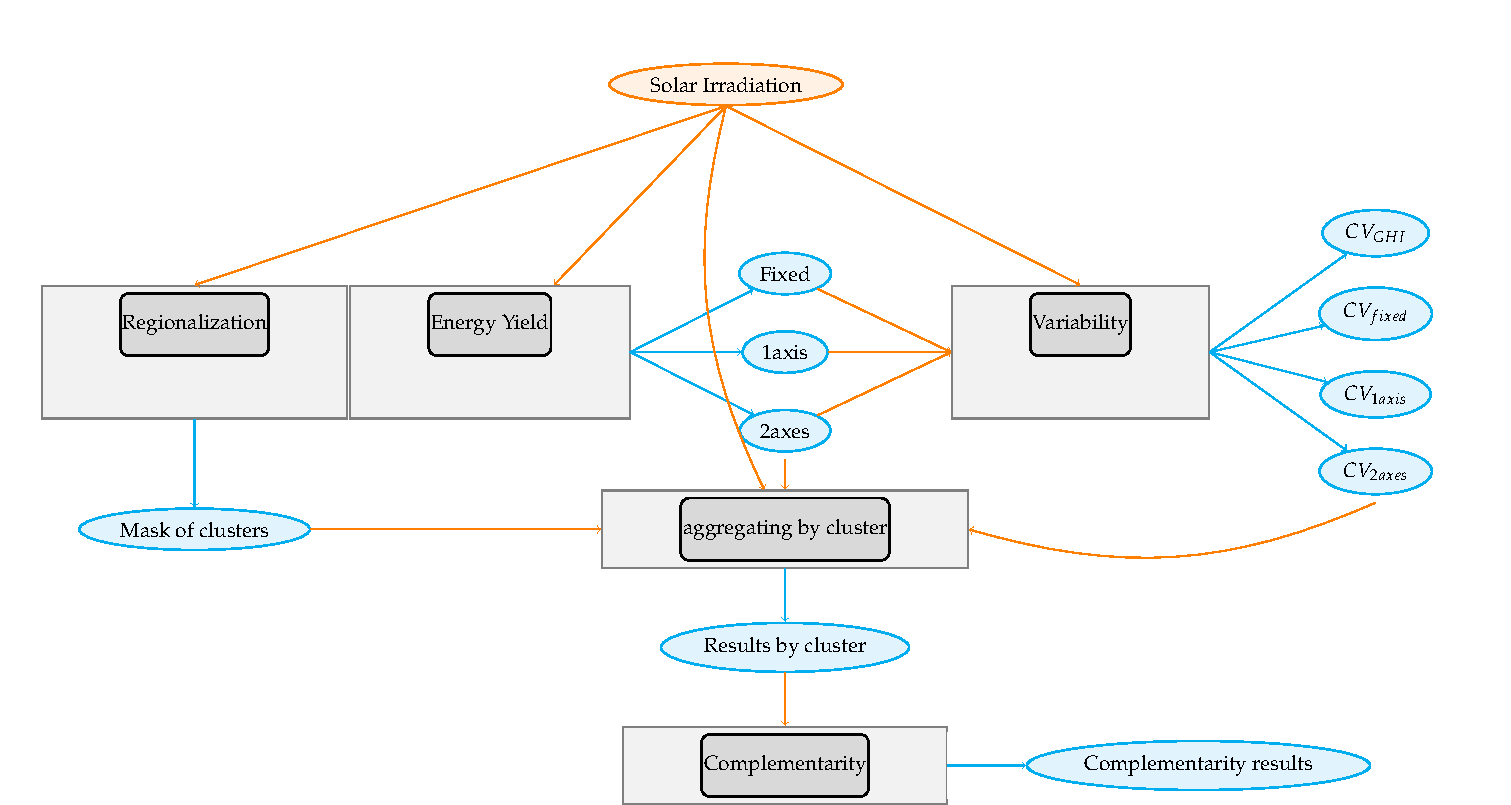
\includegraphics[width=1\textwidth]{figs/capitulo5/multi_step}
\caption{Scheme: Each gray block represents each of the operations needed to get the variability and complementarity results. Orange ellipses are the data employed and blue ellipses are the results of each stage. If the results of one of the blocks are used as input for another stage, connectors are represented in orange color.}
\label{fig:multi_step}
\end{figure}

\subsubsection{Regionalization by clustering}

Regionalization procedures provide the ability of extracting general information of the areas that could be treated as a coherent unit, facilitating the analysis and not considering those characteristics that are not under study. As it was explained in the methodological chapter, classical climatological classifications have some grade of subjectivity due to the fact that they rely on arbitrary assumptions \citep{Kottek2006} and their criteria are based on temperature and precipitation \citep{trewartha1980koppen}. For our purpose, objective and data-derived criteria are more suitable due to the fact that a different variable is analyzed and its classification does not match classical climate divisions. Objective methods based on clustering techniques have been applied successfully over the literature for the analysis of renewable energy resources \citep{Polo2015}, \citep{Zagouras2013}, \citep{Zagouras2014}, \citep{Zagouras.Pedro.2014}, \citep{gomez2015characterization} and atmospheric variables \citep{Argueso2011}, \citep{garcia2012seasonal}. \\

% Clustering methods \citep{Jain1999} can be divided into two categories, partitional and non-partitional. The partitional clustering divides the data into non-overlapping clusters while, the non-partitional or hierarchical clustering, provides a set of nested clusters. In our case, we made use of both algorithms selecting the hierarchical method to initiate a partitional algorithm that is the most suitable for our purpose: to find spatial regions that group together similar time series of the variable analyzed.

A commonly applied regionalization methodology includes the Kmeans algorithm after preprocessing the data through Principal Component Analysis \citep{Ding2004}. This two-step method first reduces redundant information by a Principal Component Analysis that decreases dimensionality of the original dataset. After that, k-means algorithm is applied to the reduced data to find the optimal partition of clusters, which is based on similarity between each element or object inside the cluster and its centroid. This is considered as the most representative element of the cluster, and similarity is measured by an objective function defined in the cluster algorithm.\\

This method presents some problems regarding the random selection of the cluster centroids in the first step. Different initial centroids can lead to different solution or a local optimum could be found. Also, there could be some computational problems if many iterations are needed to get the final partition.\\

The procedure used in \cite{Argueso2011} and in \cite{Zagouras2014} is adapted to get the optimal partition in our scheme from a combined clustering grouping and avoiding the above mentioned problems: the \textbf{k-means partitional algorithm is initialized with a hierarchical clustering solution of a the dimension-reduced data by a Principal Component Analysis.} For the particular case applied in this work, vectors of daily solar irradiation are used for the regionalization. The following steps are needed to get the optimal partition of clusters in the area:\\

\begin{itemize}
\item \textbf{To reduce data dimensionality}. Principal components are eigenvectors of an orthogonal matrix after applied a singular value decomposition (SVD) to the original data, daily solar irradiation vectors, whose initial dimension is reduced to the first eigenvectors that retain $95\%$ of the variance. Considered that, a linear combination of these eigenvectors represents the initial data.
\item \textbf{Hierarchical clustering to initialize k-means}. A hierarchical clustering method classifies data based on a hierarchy. If it is agglomerative, it will start with a cluster for each observation of the data and observations will group together recursively by similarity using the “complete linkage” method. Once the hierarchy is obtained, centroids can be calculated for each emerged partition with a number of clusters between 2 and \textit{n}, where \textit{n} is a high enough selected number of clusters. Centroids will be the initial seed for the Kmeans algorithm, avoiding the computational problems and favoring reproducibility.
\item \textbf{Kmeans algorithm}. The k-means algorithm is a partitional clustering method that minimizes an objective function that defines similarity among the elements of each cluster. In our case we made use of the Euclidean distance, Eq. \ref{eq:euclidean} between the objects or elements in the cluster and its centroid as the objective function. The number of clusters in which the data is divided into has to be known beforehand. In order to overcome the inconvenience, the algorithm is run from 2 to \textit{n} clusters and the optimum number is determined by making use of a clustering validity index after that.
\begin{equation}\label{eq:euclidean}
    J =\sum_{i=1}^{k}\sum_{j=1}^{n}{||x_i-c_j||}^2
\end{equation}


\nomenclature[J]{$J$}{Objective function of the Kmeans clustering method: summation over euclidean distances}
\nomenclature[x_i]{$x_i$}{Each point in the cluster, where the point is a vector with elements comprising the daily irradiation time series values at a pixel obtained from satellite images }
\nomenclature[c_j]{$c_j$}{Centroid of the cluster j}
\nomenclature[PV]{$PV$}{Photovoltaic}
\nomenclature[IP]{$IP$}{Iberian Peninsula}

\item \textbf{Validity index}. In order to determine the optimal partition, validity clustering techniques are applied. There are two types of validation for the clustering methods. First, external clustering validation that make use of external information out of the data; and secondly, there are internal clustering validation methods that rely only on information from the data \citep{5694060}. The latter are used to preserve objectivity as much as possible and are based on two criteria: compactness and separation of the clusters emerged. We use one of the most applied validity index, the Calinski-Harabasz index \citep{CalinskiH}, CH, that evaluates the average between and within cluster sums of squares.
\item \textbf{L-method}. CH index is calculated for every partition from 2 to $n$ clusters. The resulting CH graph in figure \ref{CHindex} for the Iberian Peninsula regionalization is shown for a number of clusters between 2 and 70 as an example. Theoretically, the partition with the maximum CH is the optimum, but the graph shows a decreasing trend which leads to imprecision in finding the optimum. The large number of data and the continuous variable analyzed are responsible for that. For that reason, the L-method is applied \citep{Salvador2004}. This method selects the intersection of two best-fit lines in the graph CH vs. \textit{k}, where \textit{k} is the number of clusters of the partition \citep{Zagouras2013}. All possible pairs of lines that fit linearly to the left and right sequence of data points are created. Each line has at least two points. The total root mean squared error is calculated as in Eq.:\ref{eq:total_RMSE}:

\begin{figure}[h!]
\centering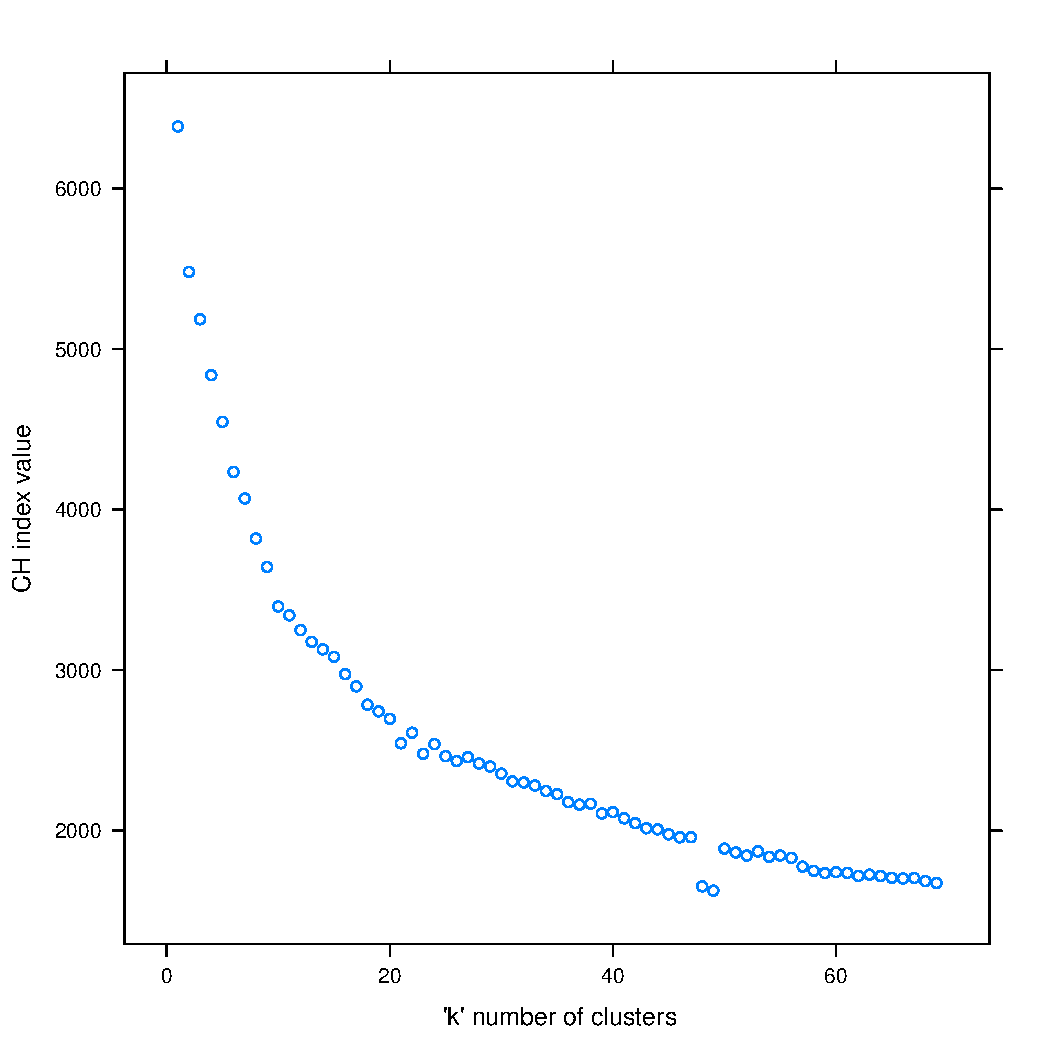
\includegraphics[width=0.5\textwidth]{figs/capitulo5/CHindex}
\caption{Calinski-Harabasz index by 'k' number of clusters}
\label{CHindex}
\end{figure}
 
\begin{equation}\label{eq:total_RMSE}
  RMSE_T = \frac{c-1}{k-1}RMSE_{left}+\frac{k-c}{k-1}RMSE_{right}
\end{equation}


\nomenclature[k]{$k$}{number of clusters.}
\nomenclature[c]{$c$}{number of clusters where the 2 fit-lines split.}
\nomenclature[CH]{$CH$}{Calinski-Harabasz validity index.}
\nomenclature[RMSET]{$RMSE_T$}{Total root mean square error}
\nomenclature[RMSEleft]{$RMSE_{left}$}{Root mean squared error of the left-side linear regression.}
\nomenclature[RMSErigth]{$RMSE_{right}$}{Root mean squared error of the right-side linear regression.}

Where \textit{c} is the number of clusters where the graph is split into the two fit-lines, \textit{k} is the total number of clusters. The ``total root mean square error'' is a weighted error with two terms, one for each side of c in the graph. Each side has a heavier weight depending on the points involved in the fitting. The minimum of $RMSE_{T}$ gives us the optimum number of clusters of the data \citep{Zagouras2013} which are used in the following steps.
 
\end{itemize}
 
\subsubsection{Photovoltaic energy yield}

The simulation of a photovoltaic energy system is described in a previous chapter. Here it is summarized in order to do not miss the coherence of the text.\\

The assessment of the power output of a photovoltaic system is carried out in two main steps:

\begin{enumerate}

\item In first place, global irradiation on the horizontal plane $G(0)$, which is the most common variable obtained from data sources, has to be transformed into the plane-of-array irradiation,  $G(\alpha, \beta)$, where $\alpha$ is the azimuth angle and $\beta$ the inclination angle of the generator plane. Due to optical losses (reflection, angle of incidence, and dust), the irradiation available is reduced for the photovoltaic cells inside the panels and the plane-of-array irradiation is then denoted as effective irradiation on the PV generator $G_{eff}(\alpha, \beta)$.\\
Three different types of tracking types are considered for the photovoltaic generator that influences on the tilt of the panels:
\begin{itemize}
\item \textbf{Fixed} panels with an optimum angle of inclination that depends on the latitude of the place.
\item \textbf{North-South} oriented panels that track the sun daily varying the azimuth angle, we will refer to them as ``one axis''
\item \textbf{Two-axes} tracking system that allows variation of the azimuth and inclination angles, we will refer to them as ``two axes''.
\end{itemize}
  
\item Once the effective irradiation that reach solar cells has been assessed, second step is the transformation into power output that depends on the photovoltaic system. The photovoltaic system is composed of a PV generator, consisting of several PV modules, and an inverter to transform the DC current output from the generator into AC current to be integrated into the network. In order to estimate  potential for photovoltaic production, the term \textit{yield} is defined as the system energy produced divided by the power installed $[\si{\kilo\watthour\per\kilo\wattpeak}]$.

\end{enumerate}

%The detailed description of the transformation from global irradiation in the horizontal plane to global effective irradiation, as well as the methods to assess power output from the PV generator are in the appendix A.

\subsubsection{Variability and complementarity}

The metric to analyze interannual variability is the coefficient of variation, CV Eq.\ref{eq:CV}, which is defined as:

\begin{equation}\label{eq:CV}
  CV=\frac{\sigma}{\overline{X}}
\end{equation}

In this equation, $\sigma$ is the standard deviation of the variable analyzed and it is divided by the mean of the variable in the period of the study. Sometimes CV is represented in percentage. This measure is dimensionless and can be applied in different time scales, which is helpful for comparisons.\\

To assess complementarity of the solar resource in the area of study, the Pearson's correlation coefficient between the time series of pairs of clusters Eq.\ref{eq:pearson} is calculated:

\begin{equation}\label{eq:pearson}
  \rho_{i,j}=\frac{\sigma_{c_i,c_j}}{\sigma_{c_i}\sigma_{c_j}}
\end{equation}

In this equation, $c_i$ and $c_j$ are the time series corresponding to the clusters $i$ and $j$. The concept of complementarity is associated with negative correlations between sub-regions of a wider area. If there is such a complementarity, a positive change in the variable for one of the clusters will be associated to a negative change for the other one. This is relevant for identifying spatial compensation possibilities and reducing overall variability in a network with high penetration of solar PV energy.\\

Complementarity can occur in different scales, either spatial or temporal and to understand it sometimes is a matter of balance. Spatial resolution for the complementarity assessment must be high enough to make sense of the comparison between zones, due to the fact that it is clear that geographically dispersed areas, far from each other, will have very different evolution of atmospheric variables, but may not be interesting from the electricity generation point of view. On the other hand, if the area of study is too small, atmospheric variables and therefore renewable resources will evolve in a very similar way. For such small areas, local complementarity between different resources can be analyzed, but not spatial complementarity of one resource. The methodology presented here addresses this issue by applying the inter-cluster comparison, that ensures homogenity within each cluster and differences between them.\\

Correlation coefficient for a long time series may hide changes in complementarity for shorter sub-periods with higher frquency correlations. For that reason a moving window is applied to the time series calculating the correlation coefficient and providing an indication of how complementarity between clusters varies during the whole period. Width of the window depends on the length of the time-series analysed.\\

In order to obtain the more important cluster pairs regarding complementarity, the median of the correlation coefficient series is calculated for each pair. After that, the cluster pairs are reordered from lower to higher values of this median correlation.\\
%, and the first 15 pairs (with the lowest median correlation) are selected as the most representative of complementarity, altought this number is rather arbitrary and also depend on the length of the time-series analysed.
 

\subsection{Results}

The optimal partition after having applied the clustering method is represented in figure \ref{clusters}. The CH validation procedure gives an optimum number of 19 clusters for the area, where each of the clusters has an homogeneous time evolution of solar irradiation. Due to the nature of clustering techniques, there is not an unique/best method to select the optimum partition. Another index (Davies-Boudin, \cite{davies1979cluster}) has been applied for comparison, and the obtained optimum number of clusters was of the same order than for CH index.
 
\begin{figure}[h!]
\centering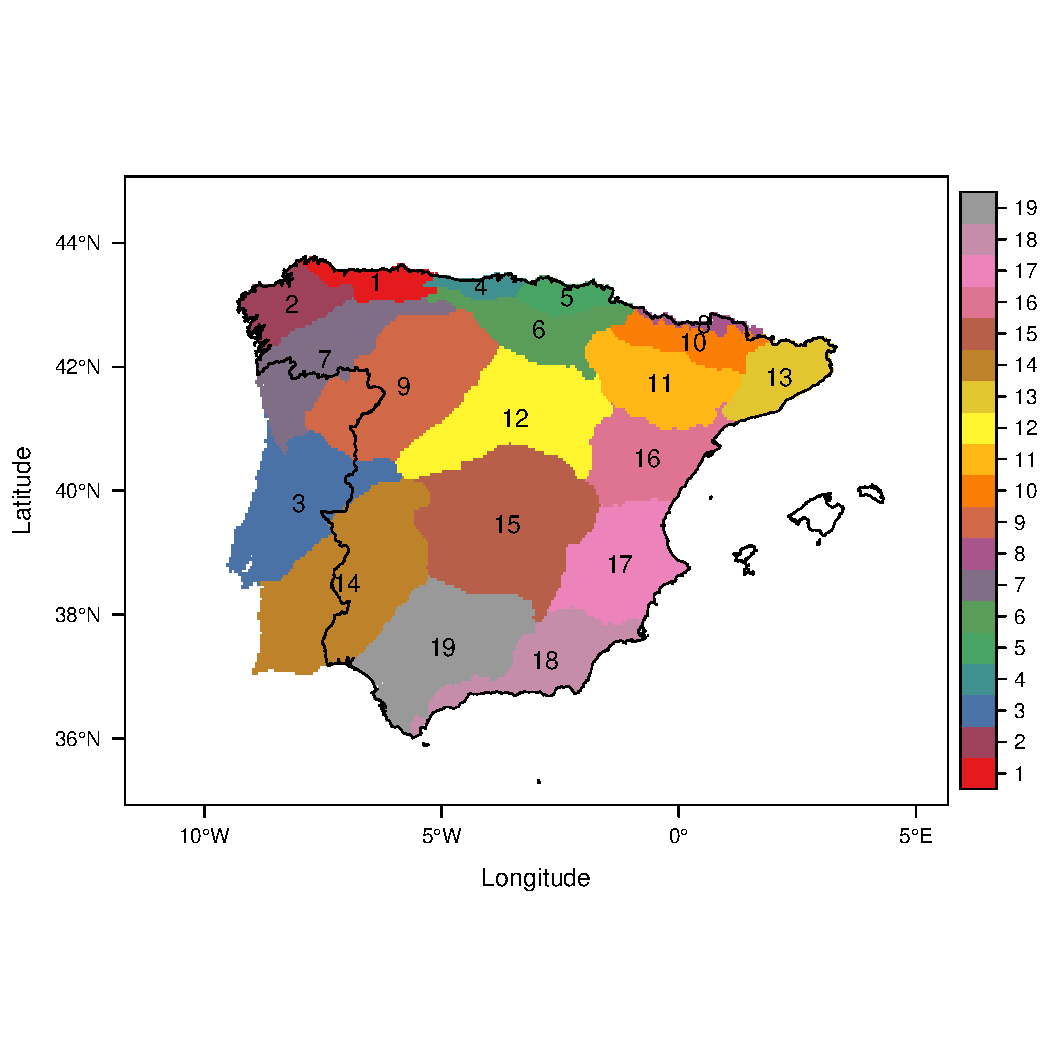
\includegraphics[width=0.6\textwidth]{figs/capitulo5/clusters2}
\caption{Optimal partition of 19 Clusters after applied the algorithm and the validity index}
\label{clusters}
\end{figure}

\subsubsection{Variability and complementarity results}

After regionalization, it is performed an analysis of solar irradiation on the horizontal plane and PV yield by tracking system, including their temporal variability.\\

Regarding interannual variability, we have calculated the CV of two time-aggregated means of solar irradiation and PV yield:

\begin{itemize}
\item On one hand it is applied for the yearly mean of daily irradiation $G_{d,y}(0)$ and yearly PV yield. This metric gives the variation of the of energy from one year to another and if it is low, general stability of the solar resource and PV production is guaranteed. 
\item On the other hand the interannual variability of the monthly time series $G_{d,m}(0)$ and monthly energy yield is also investigated in order to quantify differences in the annual cycle. 
\end{itemize}

The CV is also aggregated by cluster, in order to facilitate the intercomparison among areas.\\

%The general results about yield and variability can be found in the appendix. Here we present particularly relevant results that show the importance of considering different types of tracking methods, which is a fundamental aspect of the proposed scheme.\\

Power from the PV generator depends quasi-linearly with solar irradiation at the plane-of-array ($G_{eff}(\alpha,\beta)$), besides second order effects (spectrum, wind, etc) \citep{Perpinan2007} . Due to that the fixed typology is the one with lower yield because the amount of irradiation reaching cells is lower than the amount of energy reaching panels when trackers have one or two axes movements.

For areas where solar irradiation is higher, yield differences between trackers are higher. This can be seen in figure \ref{yearly_productivity_byCluster} where yearly mean yield for the 30-years period is aggregated by cluster and tracking system, and clusters are sorted vertically from less to more energy yield. A noteworthy result is that yield increase from fixed panels to one-axis panels is non-linear. This increase ranges between $17\%$ for the clusters with less solar irradiation, located at the northern coast (clusters 4, 5), and $30\%$ for the southern clusters with more solar irradiation (clusters 18, 19). In contrast, enegy yield increase from one-axis to two-axes panels is almost constant, around $12\%$ for all clusters. A consequence of the non-linear PV yield increase from fixed to one-axis panels is that the energy yield differences between clusters are much higher for tracking than for fixed systems. While for fixed panels PV energy yield varies between 1000 and 1450 $[\si{\kilo\watthour\over\kilo\wattpeak}]$, for two-axes systems it varies between 1350 and 2100 $[\si{\kilo\watthour\over\kilo\wattpeak}]$. These average values are coherent with results obtained in \cite{Antonanzas-Torres2013} when considering a value of 0.75 for the system performance ratio.
 
\begin{figure}[!tbp] 
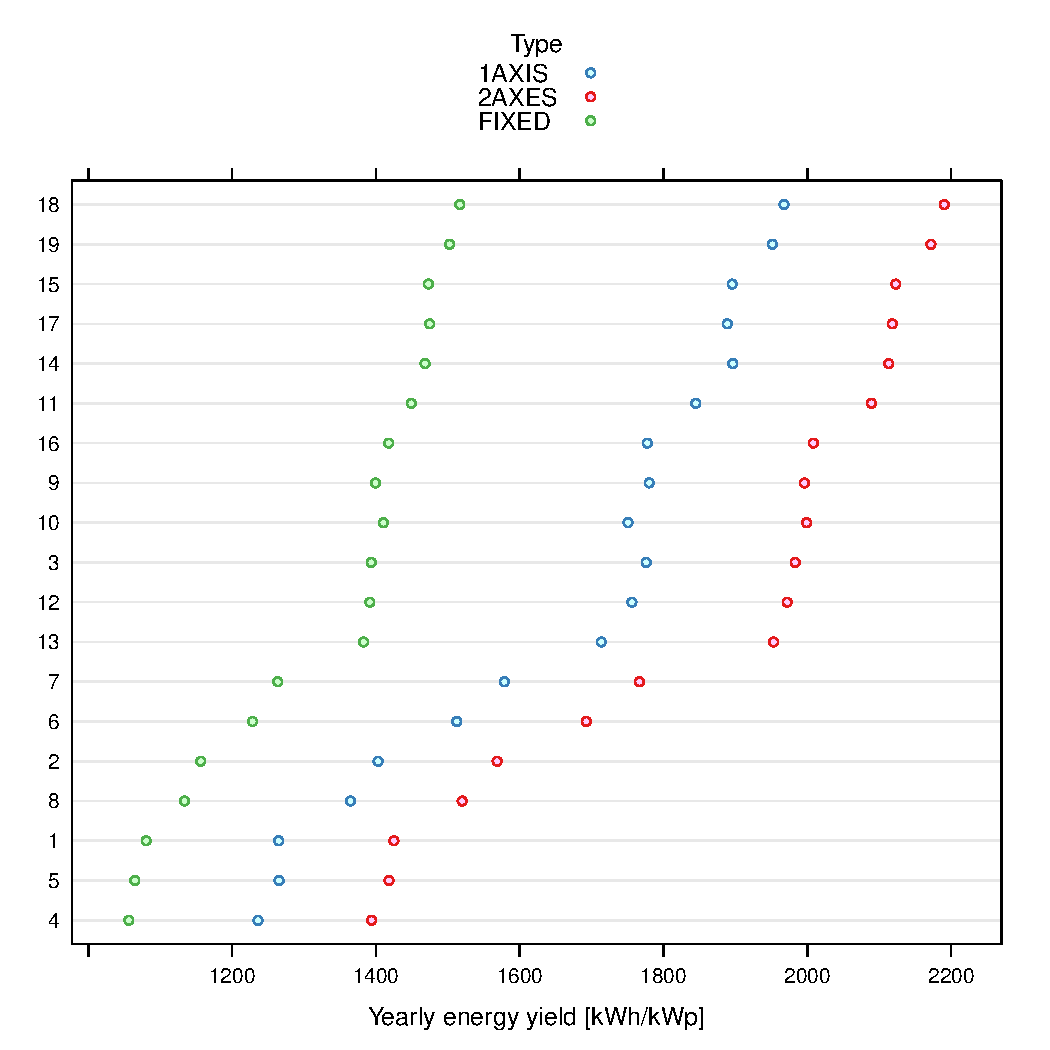
\includegraphics[width=0.6\textwidth]{figs/capitulo5/productividadTemp_byCluster.pdf}
\caption{Yearly mean of PV yield by cluster and for each tracking system $[\si{\kilo\watthour\over\kilo\wattpeak}]$. Values are sort from lower to higher yield values.}
\label{yearly_productivity_byCluster}
\end{figure}

Electricity price variations significantly depend on the variations of the monthly renewable electricity production from year to year. This time-scale is also the most influenced by the large scale circulation modes for solar potential in the Iberian Peninsula \citep{Jerez2013a}. The winter half of the year, from October to March, is especially variable.

The interannual variability for monthly yield is higher than for the irradiation at the horizontal plane, as it occurred for yearly values which results are in the appendix. In winter months, these differences in CV are much higher than in summer. This behavior is more pronounced in northern areas.

In order to quantify these differences in variability between solar irradiation and solar power output, the ratio between variability of yield by tracking system and solar irradiation is represented in figure \ref{ratiosCV} for each month and cluster. If CV of energy yield is higher than CV of solar irradiation, values are above one. On the other side values will be below one if CV of solar irradiation is higher than CV of energy yield. 

\begin{figure}
  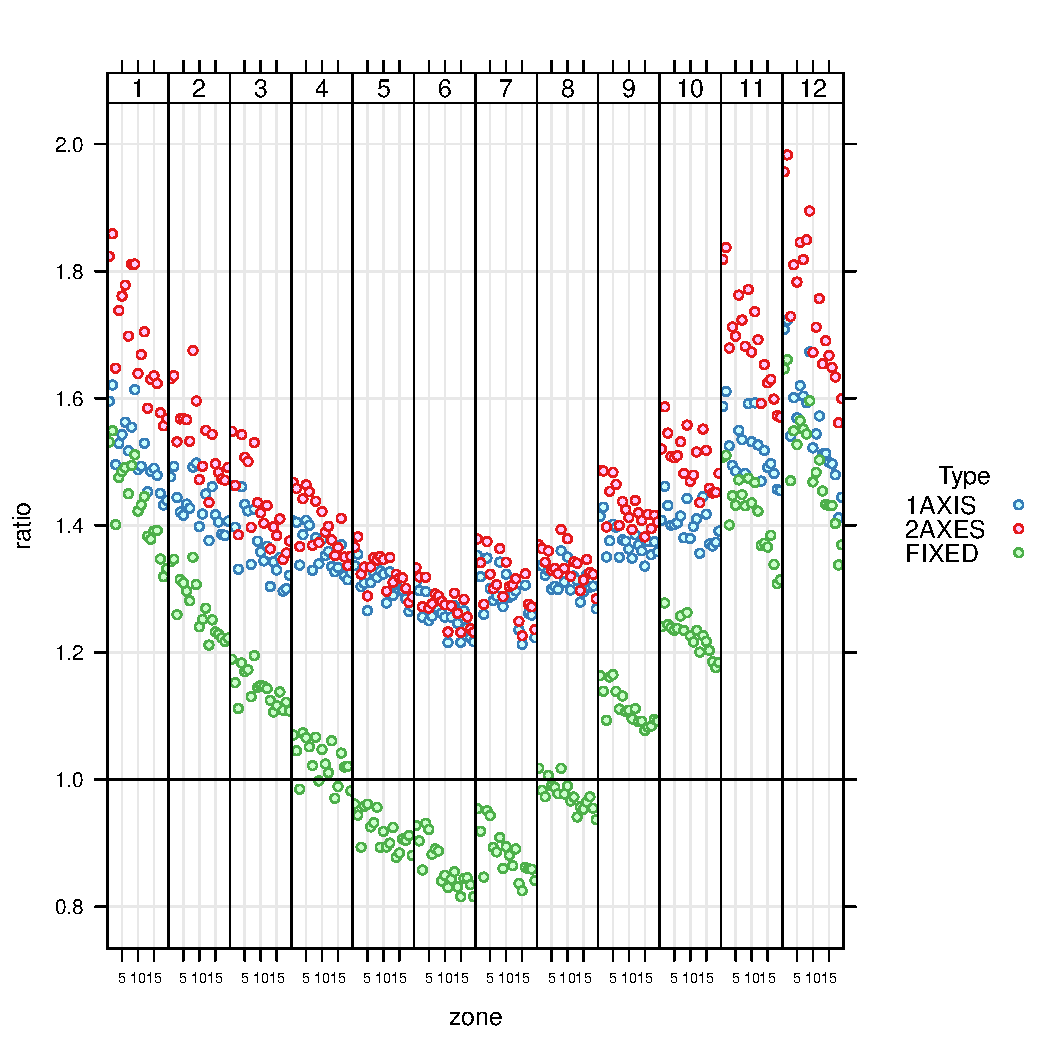
\includegraphics[width=0.6\textwidth]{figs/capitulo5/dotplot_ratio_zone.pdf}
  \caption{CV ratios between each type of tracking system and solar irradiation at the horizontal plane, grouped together by month in the graph. Ratios are calculated for each cluster, represented in the x axis. ``Fixed'' represents $\frac{CV_{fixed}}{CV_{G0}}$, ``1 axis'' is $\frac{CV_{1axis}}{CV_{G0}}$ and ``2 axis'' is $\frac{CV_{2axes}}{CV_{G0}}$}
  \label{ratiosCV}
\end{figure}

The highest ratios are obtained between $CV_{2axes}$ and $CV_{G0}$. The ratio of $CV_{1axis}$ is clearly lower in winter months, but is very similar in summer to the ratio of $CV_{2axes}$. Yield with an 'horizontal' axis tracker and 'two-axes' trackers increase the variability between $20\%$ in summer and more than $80\%$ in some areas in winter. The fixed typology ratio, $CV_{fixed}/CV_{G0}$ has a much wider range in the whole year. In winter months, it has values between 1.2 and 1.6, depending on the cluster, and is not far from the other two typologies. In contrast, this ratio decreases rapidly in summer months, reaching values below one between May and August. This means that for that period, variability of the 'fixed yield' is smaller than variability of solar irradiation at the horizontal plane.

The results of CV show that variability of PV energy yield at tilt panels is higher than variability of solar resource at horizontal plane in most cases, explained by the nature of solar irradiation at tilt panels and its dependency of solar irradiation at horizontal plane, \cite{Perpinan2009}.

The monthly time series are also selected for the complementarity analysis.

Regarding solar power complementarity, opposite-evolving time-series for different areas would strongly increase the reliability of the whole electric system, as shortfalls of solar irradiation in certain areas could be compensated by above-normal irradiation in others. However, this ideal situation is difficult to find in a rather limited area like the IP, at least for monthly timescales over a long time period of 30 years. In this case, the absence of correlation becomes also important, as it avoids simultaneous shortfalls or simultaneous above-normal values, and therefore softens the overall power production. The correlation matrix for the 30-year period and each month is in the appendix, showing the results for the whole period. In most cases, the correlation coefficient is highly positive, specially between pairs in the northern part of the Iberian Peninsula. For the southern part, the correlation coefficient is also positive but it decreases in July and August. There are some exceptions between the northern clusters 4 and 5 and the southern clusters 14 to 19, these pairs are only slightly correlated, not correlated or even slightly anticorrelated for some months.

Overall, southern and eastern clusters are uncorrelated at least during part of the year with northern and northwestern clusters. In some cases, the absence of correlation is found between nearby clusters: in winter months, the north-eastern cluster 11 (central Ebro valley) is uncorrelated to the closely-lying clusters 4, 5 and 8 (in the northern coast and Pyrenees). This is probably related to persistent atmospheric situations with north to northwesterly winds, that cause cloudiness in the windward clusters and clear skies in the leeward Ebro cluster, due to a foehn effect. This result points out the selective character of the clustering method.

It could be that the obtained clusters present higher complementarity in shorter sub-periods. We have divided the whole 30-year period in sub-periods of consecutive 15 years. The correlation coefficients have been calculated again for the resulting 15-year moving window, for each pair of clusters and for each month. In this way, we obtain how each correlation coefficient evolves during the 30 year period. The analysis has been applied for the four variables in the study: solar irradiation at the horizontal plane and PV energy yield for each tracking system.

The median value of the correlation coefficient series is calculated for each pair. Each serie comprises 12 monthly values for each of the 15-year moving windows. After that, the cluster pairs are reordered from lower to higher values of this median correlation, and the first 15 pairs (with the lowest median correlation) are selected as the most representative of complementarity. These cluster pairs are represented in figure\ref{horizonplot_rad}, showing the time-evolution of its correlation coefficient. These results are for solar irradiation on the horizontal plane. The corresponding figures for PV yield by tracking system are not shown due to the similar results obtained for this analysis.

\begin{figure}[h!]
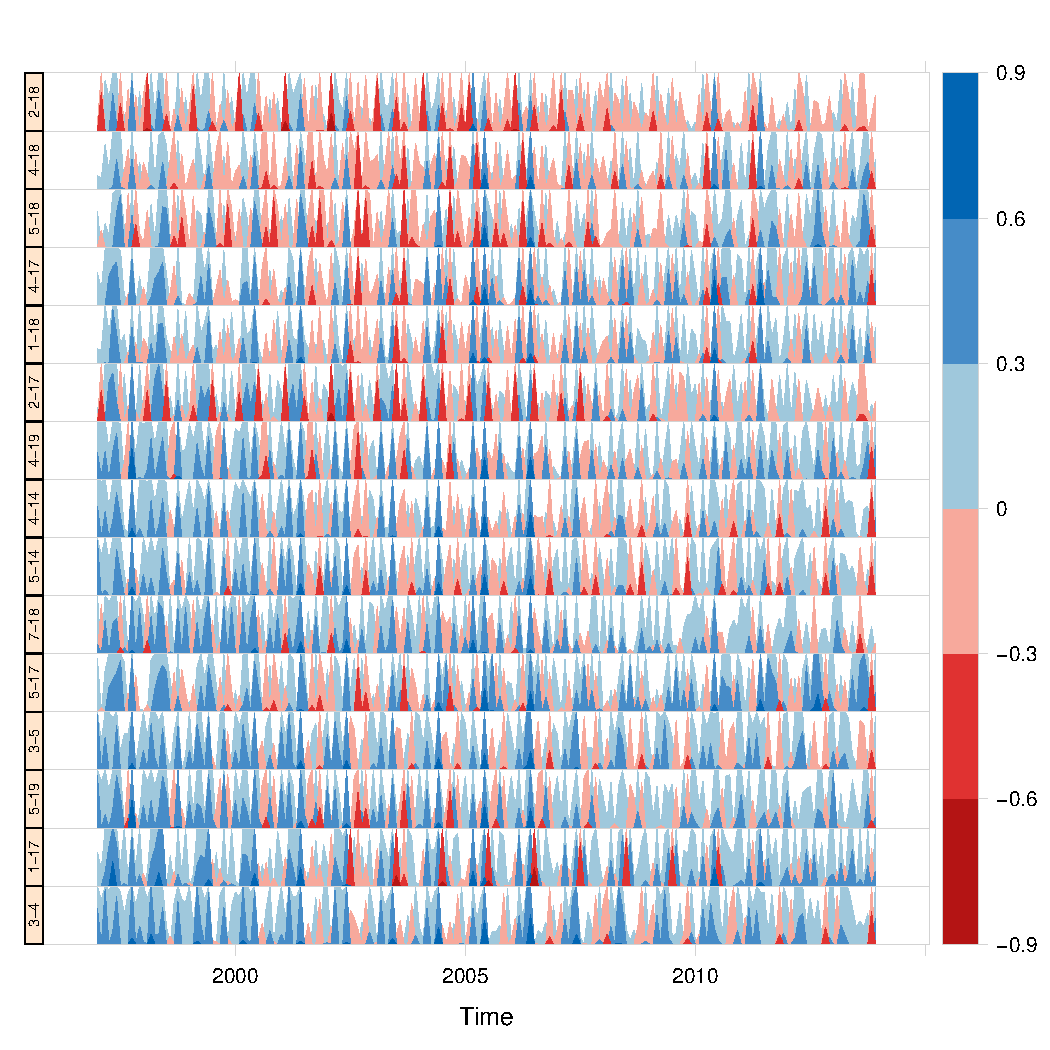
\includegraphics[scale=0.6]{figs/capitulo5/horizonplot_series_rad2}
\caption{Correlation coefficient of solar irradiation at the horizontal plane: evolution of a 15-year moving window of monthly values, for the 15 cluster pairs showing the smallest median correlation values. Monthly negative correlations (in red) and monthly positive correlations (in blue) are represented in the same axis to facilitate the comparison of the multiple time-series. Also, higher correlation values overlap with lower ones, enabling a compact presentation of all the information in a narrower plot. The cluster pairs are indicated on the left, while the year in the x-axis indicates the end of each 15-year moving window.}
\label{horizonplot_rad}
\end{figure}

The most relevant pairs in terms of complementarity include a northern (1, 2, 4 or 5) and a south-eastern cluster (17 or 18), as can be seen in figure \ref{horizonplot_rad}. The negative correlations for these pairs reach values below -0.6, at least in some 15-year sub-periods. These clusters are negatively correlated in most cases. Clusters 19 and 14 (southern and south-western IP) are also negative correlated with clusters in the north, although with lower values than the south-eastern clusters.

It is important to notice the appearance of cluster pairs 3-4 and 3-5 in this figure. These clusters are closer than the previously commented cases, which highlights the adequacy of the clustering method. All three are Atlantic coast clusters, but while cluster 3 includes part of the western coast, clusters 4 and 5 are northern coast areas. This fact, together with the position of the main mountain ranges, can explain their partially complementary behaviour.

%It is important to notice the appearance of cluster pairs 3-4 and 3-5 in this figure. These clusters are closer than the previously commented cases.  All three are Atlantic coast clusters, but while cluster 3 includes part of the western coast, clusters 4 and 5 are northern coast areas. This fact, together with the position of the main mountain ranges, can explain their partially complementary behavior. On the other hand, the 15-year moving window reveals interesting changes with time for all the cluster pairs, as there are higher and more frequent negative correlations in the middle 15-year sub-periods (those ending around 2005). 

In order to highlight the months with maximum anti-correlation,  figure \ref{horizonplot_months_rad} presents, for the same 15 cluster pairs as above, the minimum values of the monthly correlation coefficient (where the minimum for each month is calculated over all 15-year sub-periods). Differences between months are clearly observed in this graph. Only two months (March and June) show consistently positive values of this parameter, and therefore a low complementarity. In the other months, this parameter has predominantly negative values, revealing a certain degree of complementarity. July, August and September show rather low values and relatively high complementarity, which is important as these are months with a high productivity and also include the summer demand peak. In general,  for the second half of the year, the values of this minimum correlation value are lower than for the first half of the year.

\begin{figure}[h!]
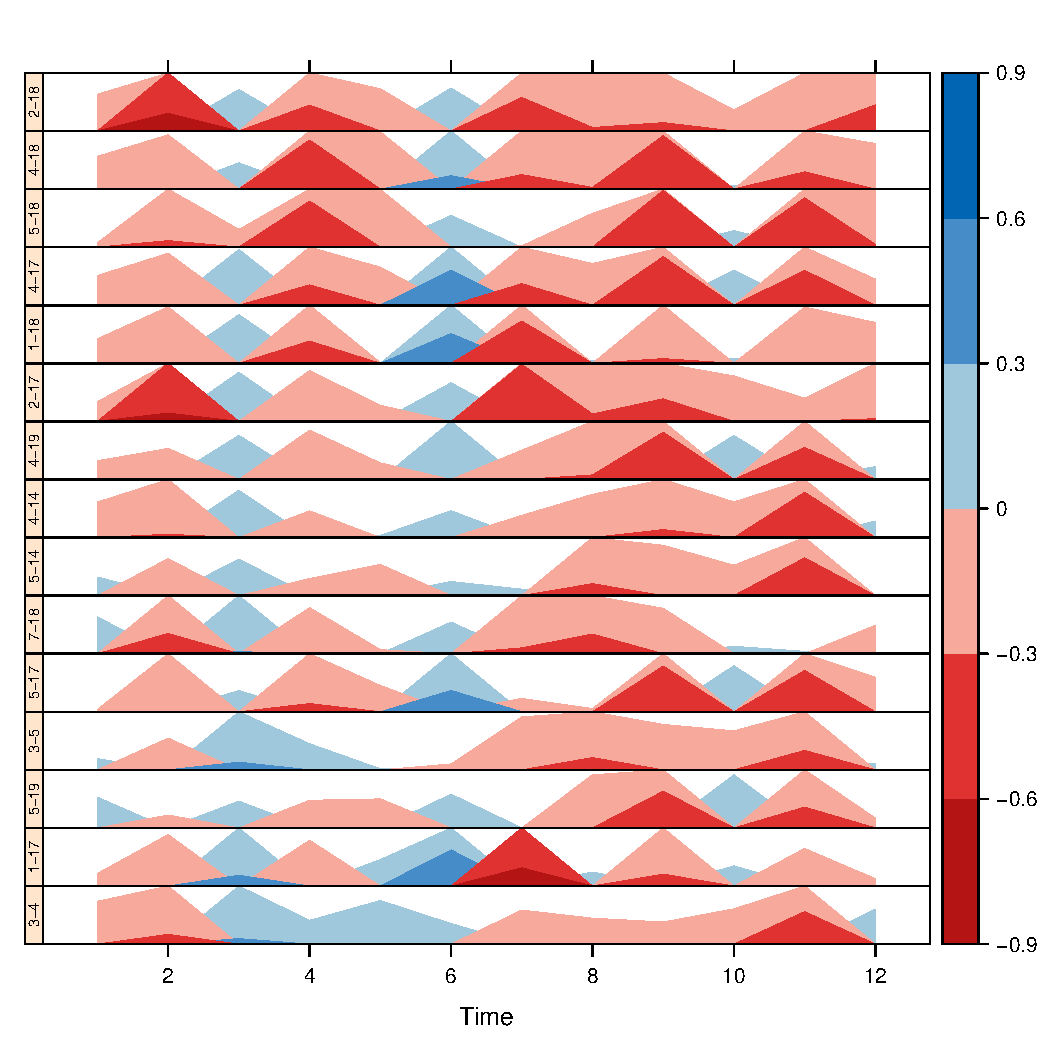
\includegraphics[scale=0.6]{figs/capitulo5/horizonplot_months_rad2}
\caption{Correlation coefficient of solar irradiation at the horizontal plane: minimum values of the monthly correlation coefficient, for the same cluster pairs as figure \ref{horizonplot_rad}. The minimum is calculated over all 15-year sub-periods. The type of representation of correlation values is the same as in figure \ref{horizonplot_rad}. The cluster pairs are indicated on the left, while the numbers in the x-axis indicate the months.}
\label{horizonplot_months_rad}
\end{figure}



\subsection{Conclusion}
\subsection{Summary}

\chapter{Impact of aerosols in photovoltaic energy production over the Euro-Mediterranean area}

\begin{abstract}

The increase in the photovoltaic energy installed capacity over the world leads to the need of a better understanding of solar resource and its variability. The aim of this work is to assess the influence of aerosols on photovoltaic energy production from seasonal to multi-decadal time scales. For this purpose we use various coupled aerosol-climate simulations that take into account the complex spatial and temporal patterns of natural and anthropogenic aerosols over the Euro-Mediterranean domain.

The results show that aerosols strongly influence the spatial pattern, seasonal cycle and long-term trend of PV production. The most affected area is Central Europe where sensitivity of PV production to aerosols is higher. The annual production loss due to aerosols ranges from no impact to $-16\%$ in The Netherlands, with variation depending on the area and on the typology of the tracking system. The summer production loss can even reach $-20\%$ over regions of Africa and Syria-Iraq.  

We conclude that aerosols can not be neglected in the assessment of PV production at large time scales over the Euro-Mediterranean area. Besides, the potential increase in energy due to reduction in the antrophogenic aerosols is shown in the simulation of the brightening period over Europe, with an increase of 2000 ${\kilo\watthour\over\kilo\wattpeak}$ in a PV lifetime for the most affected areas. It illustrates the evolution that PV potential could follow in highly polluted areas through the effective implementation of pollution control measures.  
  
   
\end{abstract}
 
\begin{keyword}
\texttt{Photovoltaic production variability\sep Aerosols\sep Regional Climate Modeling}
\end{keyword}

\end{frontmatter}

\linenumbers

\section{Introduction}


In the last decades there has been an overall increase in the deployment of photovoltaic (PV) power plants over the world, demanding research in the fields that contribute to a better integration of this technology into the electricity system. Due to the variability of solar resource, a comprehensive study of its spatiotemporal behavior is needed.

Aerosols particles influence the climate system directly, affecting the Earth’s radiation budget by scattering or absorption of solar radiation, or indirectly, changing cloud properties. Due to their importance in the amount of solar radiation that reaches the Earth’s surface and their effect in the changing climate, the evaluation of their impact on the solar resource for energy purposes is of special interest.

A general lack of well-spread surface stations, which provide solar radiation measurements, has made the satellite information the main and most reliable source of data up to now, due to its spatial and time resolution \citep{Posselt2012, Ineichen2014}. However, satellite retrievals were not available several decades ago and they do not allow to quantify the effect of specific factors on solar irradiance. Thus for investigating long-term statistics and to disentangle the various factors influencing solar resource, a different approach is needed. Models are the best tool to understand processes that occur in the atmosphere and their link with the resource variability, as individual factors can be included or removed in them, allowing the isolation of their effects.

Due to the increasing concern about the availability of renewable energy resources under climate change scenarios, climate modeling has revealed itself as a valuable tool for evaluating future energy potential \citep{Crook2011, Gaetani2014, Gaetani2015, Jerez2015, Jerez2015climix, Tobin2016}. However, representation of the clouds is still one of the main challenges for these models, and the spatio-temporal variability of aerosols is rarely taken into account in some of regional climate models \citep{Bartok2017}, which could lead to significant errors in PV power forecasting or future energy estimations \citep{Rieger2017}. Such climate simulations have to be combined with an accurate PV model capable of reproducing the system performance. Existing studies analysing the influence of aerosols on solar irradiation lack spatial detail (because of the use of relatively coarse global climate models) and/or do not apply a detailed PV production model \citep{Bergin2017}. 

The Mediterranean region is considered as highly influenced by aerosols coming from different sources \citep{Lelieveld}. These aerosols have a deep impact on the climate of the region \citep{Nabat2014, Nabat2014a}, thus on the shortwave solar radiation reaching the surface \citep{Mallet2016}. Regarding possible changes in antrophogenic aerosols in the future \citep{Gaetani2014, Jimenez-Guerrero2011}, the relevance of the near-term climate change scenarios and the expected PV deployment, the study of the Euro-Mediterranean area is important for solar energy.

In this work we use a regional climate model \citep{Nabat2014} with a realistic aerosol representation combined with an accurate PV model \citep{Lamigueiro2012}. The influence of these aerosols in the spatiotemporal variability of PV production over the region is quantified. The analysis is made in present climate conditions for simulations between 2003 and 2009 and different tracking types are considered in the study, due to the different sensitivity of each typology to changes in solar radiation \citep{Gutierrez2017}. On the other hand, the impact that trends in antrophogenic aerosols have in PV energy production is also investigated using longer simulations for the ``brightening'' \citep{Wild2005} period, 1980-2012, reflecting how pollution control policies could benefit the PV energy production in highly polluted areas.

This paper is organized as follows: in section 2 the climate and the photovoltaic model are described. In addition, there is a description of the aerosols and the datasets used for evaluation. Section 3 presents the results and shows the impact of aerosols on photovoltaic energy production. It is organized depending on the space-time scale analysed and there is a subsection for the tracking system sensitivity.  Flinally, section 5 is a discussion section for limitations and future perspectives and section 6 shows the main conclusions.

\section{Data and Methods}

Different climate simulations are used as an input of a PV power model. These climate simulations provide the daily-mean shortwave solar radiation, SSR, at the surface. The energy production model simulates the performance of a general photovoltaic system and includes different tracking types, considering the tilt of photovoltaic panels as a relevant component of the whole assessment. Computation of the photovoltaic energy model is made using the R open-source package named solaR \citep{Lamigueiro2012}.

\subsection{Climate Data}

The climate model used in this study (CNRM-RCSM4,\citep{Sevault2014}) is a coupled Regional Climate System Model (RCSM) dedicated to the study of the Mediterranean climate. CNRM-RCSM4 is one of the RCSMs contributing to the multi-model Med-CORDEX initiative \citep{Ruti2016}. It has the specificity to represent various components (atmosphere, land surface, river, ocean) of the Mediterranean regional climate system at high-resolution as well as their high-frequency coupling. The horizontal resolution is 50 km for the atmosphere, the land surface and the river network, and about 10 km for the Mediterranean Sea. In addition, the atmosphere part of the model, the so-called ALADIN-Climate version 5.2 \citep{Colin2010} is one of the few available Regional Climate Models which can take into account a realistic representation of the spatiotemporal variability of the aerosols \citep{Nabat2014}. The model has been extensively described, evaluated and intercompared with other Med-CORDEX models in previous studies, \cite{Sevault2014, Nabat2014, Nabat2014a,Flaounas2016, Gaertner2016, DellAquila2016, Harzallah2016, Cavicchia2016}

The detailed interannual aerosol dataset used in the climate simulations \citep{Nabat2013}, NAB13, is able to reproduce the spatiotemporal variability of AOD (aerosol optical depth) over the Mediterranean region. It improves the representation of aerosols against older climatologies commonly applied in regional climate studies like \cite{Tegen1997} or \cite{tanre1984first}.

The NAB13 dataset includes five different aerosol species: Sea Salt, Black Carbon, Sulfate, Organic Carbon and Desert Dust (ss, bc, su, or, sd); with spatial and temporal variability. It is based on a blending of a satellite-derived AOD product and a high-resolution regional climate model using up-to-date interactive aerosols module. This dataset has also been evaluated against ground stations \citep{Nabat2013}.

During the eighties, some policies against the emissions of certain types of antrophogenic aerosols were implemented in Europe, which has been linked with the observed increase in the shortwave solar radiation in the area \citep{Wild2005}. For simulations over this commonly named ``brightening period'' (1980-2012), a trend for sulfate aerosols is included in NAB13, being able to reproduce the shortwave solar radiation trend observed over Europe since 1980 \citep{Nabat2014a}.

There is a large spatial and seasonal variability of the AOD at 550nm over the Euro-Mediterranean. Spring and summer months are highly influenced by dust aerosols in the south of the domain. In winter, antrophogenic aerosols dominate in central Europe and during autumn, there are few areas with high values in opposition to the rest of the domain.

The domain considered in the simulations covers the Mediterranean area in addition to a large part of Europe (see figure \ref{fig:mapapral}).

For the first period, 2003-2009, a pair of runs is analysed. We refer to them as \textbf{AER} and \textbf{NO-AER}. The AER simulation includes the NAB13 dataset, whereas no aerosols are included in NO-AER. This pair allows to easily attribute the obtain differences to the aerosols effect, therefore to quantify the impact of aerosols on the Euro-Mediterranean SSR and PV productivity. It is an important point considering the fact that some of the state-of-art RCM do not include aerosols in their simulation, so it gives an idea of that missing forcing.

Secondly, a longer simulation between 1980 and 2012, \textbf{TREND}, covering the ``brightening'' period observed in Europe is also analysed. It will show the effect of a decreasing trend in sulfur aerosols on the shortwave solar radiation and on the PV productivity.  

A summary of the different simulations is reported in table \ref{tabSIM}.

\begin{table}
  \begin{tabular}{>{\raggedright}m{2cm}>{\raggedright}m{3cm}>{\raggedright}m{2cm}}
    \toprule 
    Simulation & Aerosols & \centering{Period}\tabularnewline
    \midrule
    AER & NAB13 & 2003-2009
    \tabularnewline
    \midrule
    NO-AER & Not included & 2003-2009
   \tabularnewline
   \midrule           
  TREND & NAB13 + sulfates trend & 1980-2012
   \tabularnewline
    \bottomrule
  \end{tabular}
  \caption{Simulations of the CNRM-RCSM4 regional climate model to obtain SSR and temperature as input of the photovoltaic model, period and representation of aerosols in each simulation.}
\label{tabSIM}
\end{table}

\begin{figure}[h!]
\centering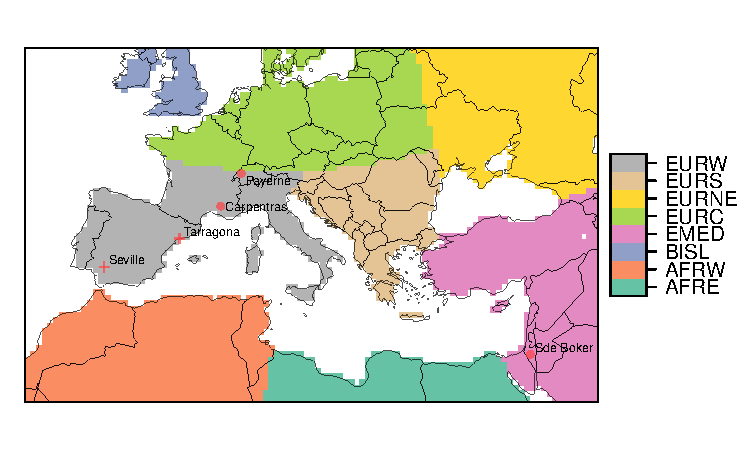
\includegraphics[width=0.7\textwidth]{figs/capitulo6/zonasPuntosLabel.pdf}
\caption{Areas defined to evaluate the difference in solar radiation between the satellite and the climate model simulations: Western Europe, EURW; Southern Europe, EURS; North-Eastern Europe, EURNE; Central Europe, EURC; Eastern Mediterranean, EMED; British Island, BISL; Western Africa, AFRW; Eastern Africa, AFRE. The location of the BSRN stations is represented with points ``.'' and the two PV plants are plotted with ``+'' in orange.}
\label{fig:mapapral}
\end{figure}

 
\subsection{PV model description}

In this section we make use of the commonly used terms: shortwave solar radiation, SSR, is equivalent to the global irradiation at the horizontal plane $G(0)$, which is composed of the beam component, $B(0)$, the diffuse irradiation, $D(0)$, and the albedo $R(0)$.

A photovoltaic energy system is mainly composed of the generator, consisting of several modules that include the cells to transform solar radiation into electricity, and the inverter, which transforms direct current into alternate current to be integrated into the electricity network. The assessment or estimation of the power output of a PV system implies modeling its components. For this purpose, two main steps have to be considered. The first is related to the amount of energy that reaches the generator surface and the other is based on the performance of the electrical components. The procedure is described in \cite{Perpinan2009} and the same methodology was applied in \cite{Gutierrez2017}.

1) Global irradiation at the horizontal plane $G(0)$, as an output of the climate model, has to be transformed into the global effective irradiation, $G_{eff}(\alpha, \beta)$, which is the amount of energy reaching the tilted surface of the generator (where $\alpha$ is the azimuth angle and $\beta$ the inclination angle) after considering reflection losses, angle of incidence and accumulated dust.  

First, for the decomposition of $G(0)$, empirical equations that correlates the \textit{clearness index} and the \textit{diffuse fraction} \citep{Page1961} are used. The clearness index is a measure for the energy lost when solar irradiation goes through the atmosphere, and the diffuse fraction is the relationship between the diffuse component, $D(0)$, and the global irradiation at the horizontal plane $G(0)$. Its value is the amount of the diffuse component in global irradiation.

The equations that relate the clearness index to the diffuse fraction depend on the place and time scale involved. There are many relationships proposed depending on the area of the study \citep{deMiguel2001, Gopinathan1995}. For daily time-scales, the equations that relate the clearness index and the diffuse fraction proposed by \cite{Aguiar1992} are used in our case. 

Three different tracking types are considered for the photovoltaic generator and the equations describing movements and relative position between the system and the sun are described in \cite{Perpinan2009}
\begin{enumerate}
\item \textbf{Fixed panels} with an optimum angle of inclination that depends on the latitude.
\item \textbf{One} axis trackers, with a generator rotating on an axis oriented North-South. We will refer to them as \textbf{“one”}.
\item \textbf{Two-axes} tracking system that allows variation of the azimuth and inclination angles, we will refer to them as \textbf{“two”}.
\end{enumerate}

To obtain irradiation components in the tilted surface at daily time scale, it is first necessary to estimate the irradiance profile using empirical relationships \citep{Collares-Pereira1979}. Irradiance profile is then transformed into its components at the tilted surface and integrated in time to obtain the energy reaching the generator surface. Direct irradiance can be transformed to the tilted surface using only geometrical criteria whereas the diffuse fraction is obtained with the model proposed by \cite{hay1985estimating}. This model considers an approximation where the sky sphere is seen by the generator as isotropic except for the circumsolar region, which is considered to emit direct irradiance. The albedo component is considered as isotropic, due to the fact that its contribution to global irradiance is low. 

Finally, we apply equations from \cite{Martin2001} to obtain $G_{eff}(\alpha, \beta)$. It includes optical losses due to the fact that, except for the two-axis tracking system, the incident irradiation deviates from the normal of the generator. Also, transmittance losses are included for accumulated dust over the surface, considering a ``moderate dust degree'' in the terms used in the referenced paper \cite{Martin2001}. In this case, any spatial distinction is considered and the same coefficient values are used to calculate angular and transmittance losses. 

2) The second step is the transformation into power output, depending on the electrical characteristics of the components in the photovoltaic system and second order effects like temperature. A summary of the modules and the inverter model can be found in table \ref{table1}. Detailed information about this step can be found in \cite{Perpinan2009}.

Ambient temperature is needed since the efficiency of the cells decreases with the increase of temperature, assuming a linear relationship. In this work we use the equation of \cite{Crook2011}, to calculate the daytime temperature from the daily maximum and minimum temperature, obtaining a daily profile. 

Computation of the photovoltaic energy model is carried out with the \texttt{solaR} package \citep{Lamigueiro2012}. This package implements in R a set of functions that include the sun apparent movement equations, the solar irradiation and irradiance decomposition, transposition models, and the PV generator and inverter models. 

\begin{table}[h!]
  \begin{tabular}{>{\raggedright}m{2cm}>{\raggedright}m{6cm}}
    \toprule 
    Element & Method\tabularnewline
    \midrule
    PV generator & Identical modules with
    $dV_{oc}/dT_{c}=0,475\frac{\%}{\celsius}$ and $NOCT=47\celsius$. 
    The MPP point calculated as in \cite{garcia2005caracterizacion}). \tabularnewline
    \midrule
    Inverter & Efficiency equation proposed in
    \cite{jantsch1992results}:  
    \begin{equation}
      \eta_{inv}=\frac{p_{o}}{p_{o}+k_{0}^{o}+k_{1}^{o}p_{o}+k_{2}^{o}p_{o}^{2}}
    \end{equation}
    where $p_{o}=P_{ac}/P_{inv}$ is the normalized output power of the inverter. The characteristic coefficients of the
    inverters are: $k_{0}^{o}=0.01$, $k_{1}^{o}=0.025$, $k_{2}^{o}=0.05$.\tabularnewline
    \midrule
    Other losses & \begin{itemize}
    \item Average tolerance of the set of modules, $3\%$.
    \item Module parameter dispersion losses, $2\%$.
    \item Joule losses due to the wiring, $1.5\%$.
    \item Average error of the MPP algorithm of the inverter, $1\%$.
    \item Losses due to the MV transformer, $1\%$.
    \item Losses due to stops of the system, $0.5\%$.
    \end{itemize}
    \tabularnewline
    \bottomrule
  \end{tabular}
  \caption{Calculation procedure for the estimation of energy produced by a PV system from daily global horizontal irradiation data. Left column represents the element of the PV system and the right column the equations and methods used in each case for the efficiency of the elements.}
  \label{table1}
\end{table}

\subsection{Datasets for evaluation}
\subsubsection{Satellite product: CM-SAF.}

CM-SAF (Climate Monitoring Satellite Application Facility) \citep{Schulz2009} was created as part of EUMETSAT Satellite Application Facility (SAF) when the importance of “contributing to the operational monitoring of the climate and the detection of global climatic changes” was recognized. Besides its operational products, they provide Climate Data Records generating long-term data, which is a valuable product for climate variability studies. In this work, the SARAH \citep{Muller2015} dataset for daily shortwave solar radiation, SSR, is used with an horizontal resolution of 0.44º to be consistent with the model simulations and for the period 2003 and 2009. For this product, the $85\%$ of absolute differences with shortwave solar radiation measurements is below 10 $\watt/m^2$ for monthly values and 13 $\watt/m^2$ for daily means.

Concerning aerosols representation, the satellite dataset includes information from MACC \citep{Benedetti2009, Morcrette2009}, provided by the European Centre for Medium-Range Weather Forecasts (ECMWF). Monthly long-term means of a 0.5x0.5 degrees grid are spatially interpolated to assign the values of each pixel.

\subsubsection{BSRN stations}

The BSRN (Baseline surface radiation network) \citep{Ohmura1998} is a set of ground-based measurements, from the WRCP Radiative Fluxes Working Group. It was created for supporting research in the radiation budget of the Earth-atmosphere and the radiation distribution, considering its main role in climate processes. The main objective is to provide high-quality measurements that are able to deal with the scarcity of the existing radiometric network. Although there are not many stations available for the period of the study in the Euro-Mediterranean domain, the high quality data provided by BSRN is necessary for a first evaluation of the climate simulations.

The three stations of the BSRN network used in this study (Payerne, Carpentras and Sede Boker) covered the period 2003-2009 and provide SSR monthly data. Their location is represented in figure \ref{fig:mapapral} together with the PV plants considered in the study.  

\subsubsection{Temperature data: ECAD}

The PV production assessment calculated using the SSR from satellite data needs also the temperature for the performance of cells inside the module. The gridded E-OBS data set from the EU-FP6 project ENSEMBLES \citep{Haylock2008} is used in the energy production model at daily resolution. Mean, maximum and minimum temperature from the dataset, in a spatial resolution of 0.25º, are interpolated to the same grid of the climate model. 

\subsubsection{PV production data}

Data from two different power plants are used for the evaluation of the simulated PV power and the assessment of the added value of the aerosol inclusion in the climate simulations.

The two power plants are in the Iberian Peninsula and their location represented in figure \ref{fig:mapapral}. The first one, located in Tarragona in the North-East area, is a PV system with fixed structure. The second one is a two-axis tracking PV plant located in Seville, in the South of Spain. Details of both PV power plants are in table \ref{tabPlants}, including the electrical characteristics of their components. 

\begin{table}[h!]
  \begin{tabular}{>{\raggedright}m{1.5cm}>{\raggedright}m{3cm}>{\raggedright}m{3cm}}
    \toprule 
     & \centering{Seville} & \centering{Tarragona}\tabularnewline
    \midrule
    Type & \centering{two-axes} & \centering{fixed} 
\tabularnewline
    \midrule
    Generator & \centering{$P_{g}=27.31$ $\kilo\wattpeak$}\\ 
                 \centering{$N_{mp}=12$}\\
                 \centering{$N_{ms}=11$} & \centering{$P_g=100.18$ $\kilo\wattpeak$}\\
                               \centering{$N_{mp}=27$}\\
                               \centering{$N_{ms}=35$}
   \tabularnewline
   \midrule
   Inverter & \centering{$P_{inv}=25$ $\kilo\watt$}\\
              \centering{$V_{min}=405$ $\volt$} & \centering{$P_{inv}=100$ $\kilo\wattpeak$}\\
                                \centering{$V_{min}=450$ $\volt$}
    \tabularnewline    
    \bottomrule
  \end{tabular}
  \caption{Summary of the electrical components of the two photovoltaic plants, including generator characteristics (generator power $P_g$, and modules in parallel and serie, Nmp and Nms) and the inverter characteristics (power of the inverter $P_{inv}$ and the voltage $V_{min}$).}
  \label{tabPlants}
\end{table}


Data of PV production are difficult to obtain due to confidentiality contracts. Moreover, when data are available time series are not always complete. Maintenance, modules substitutions, inverter problems and other stops in the production may lead to common time-gaps in the datasets. These limitations must be taken into account when establishing statistical comparisons between models and real data. In this case, the two PV power plants provide daily data within the period 2003-2009, the details are in table \ref{localData}. Monthly means of these data are compared against the monthly means of simulated daily PV productivity, energy produced by the power installed ${\kilo\watthour\over\kilo\wattpeak}$, with the models and the satellite. Only months with more than 15 days of data available are considered for the monthly mean and compared against simulated data.

\section{Results} 

Although the AOD dataset and the climate simulations used in this study have already been evaluated against observations and satellite datasets in \cite{Nabat2013, Nabat2014, Nabat2014a}, an additional assessment of the SSR form the climate simulations is also made in this work against the CM-SAF SARAH dataset \citep{Muller2015} for the period 2003-2009 and against some BSRN \citep{Ohmura1998} stations at a local scale. 
\subsection{Local scale}

Three different stations from BSRN cover the period between 2003-2009 with SSR monthly data. Stations are represented in figure \ref{fig:mapapral} with points. Also, two different power plants in Spain, represented in figure \ref{fig:mapapral} with a cross, are used to evaluate PV power simulations at a local scale. A summary of the data used in this section, the periods and the resolution can be found in table \ref{localData}.


\begin{table}[h!]
  \begin{tabular}{>{\raggedright}m{2cm}>{\raggedright}m{2cm}>{\raggedright}m{2cm}>{\raggedright}m{2cm}>{\raggedright}m{2cm}>{\raggedright}m{2cm}}
    \toprule 
    Data from & \centering{Seville} & \centering{Tarragona} & \centering{Payerne} &\centering{Sede Boker} &\centering{Carpentras}\tabularnewline
    \midrule
    Variable & \centering{PV productivity} & \centering{PV productivity} & \centering{SSR} & \centering{SSR} & \centering{SSR} 
\tabularnewline
    \midrule
    Time res. & \centering{day} & \centering{day} & \centering{month} & \centering{month} & \centering{month}
                    \tabularnewline
   \midrule
                                                                                            Period & \centering{518 {\small{daily values between:}} 02-07-2007\\30-11-2008} & \centering{300 {\small{daily values between:}} 01-01-2003\\19-03-2005} & \centering{2003-2009} & \centering{2003-2009} & \centering{2003-2009}
                  \tabularnewline    
 \midrule
    $\%$ no data & \centering{0} & \centering{8 $\%$} & \centering{0} & \centering{10.71 $\%$} & \centering{0}
                    \tabularnewline

 \bottomrule
  \end{tabular}
  \caption{Summary of the local data of PV power plants and SSR from BSRN stations used for the evaluation of the simulations. SSR is evaluated as input of the PV model and the PV output as the result of the whole modeling process.}
  \label{localData}
\end{table}

In figure \ref{fig:station} differences in monthly time series of SSR from simulations and satellite data and the stations measurements are represented.

\begin{figure}[h!]
  \centering\begin{subfigure}{0.4\textwidth}
    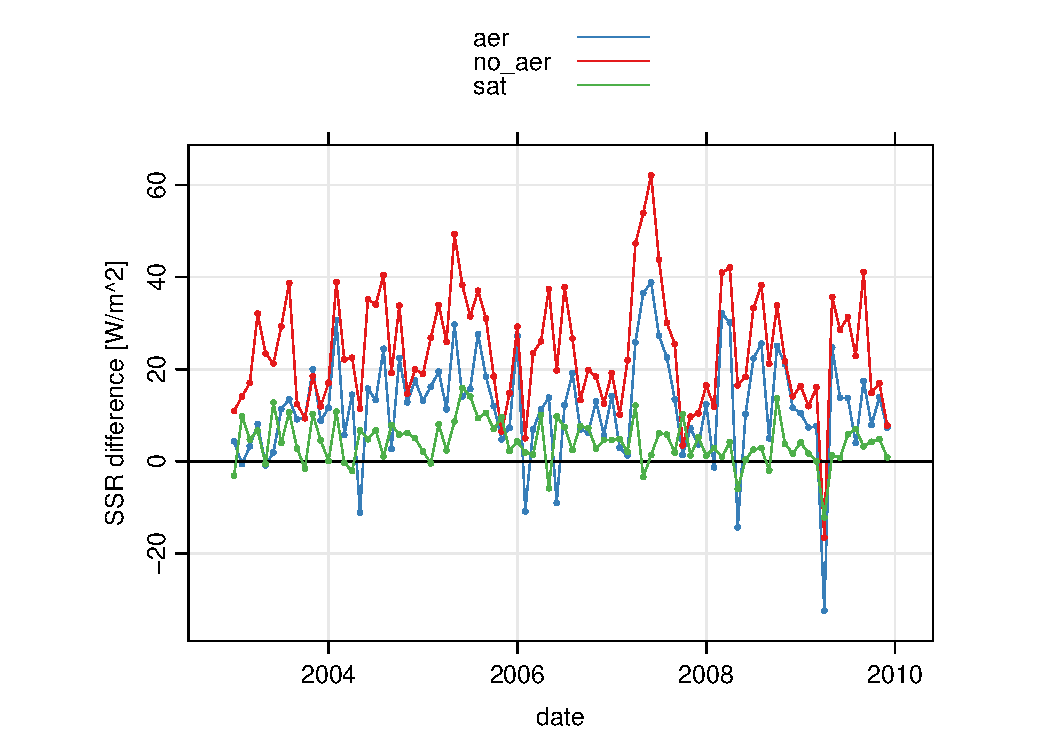
\includegraphics[width=1.2\textwidth]{figs/capitulo6/CarpentrasMesesDif.pdf}
    \caption{Carpentras}
    \label{Carpentras}
  \end{subfigure}
  %
  \centering\begin{subfigure}{0.4\textwidth}
    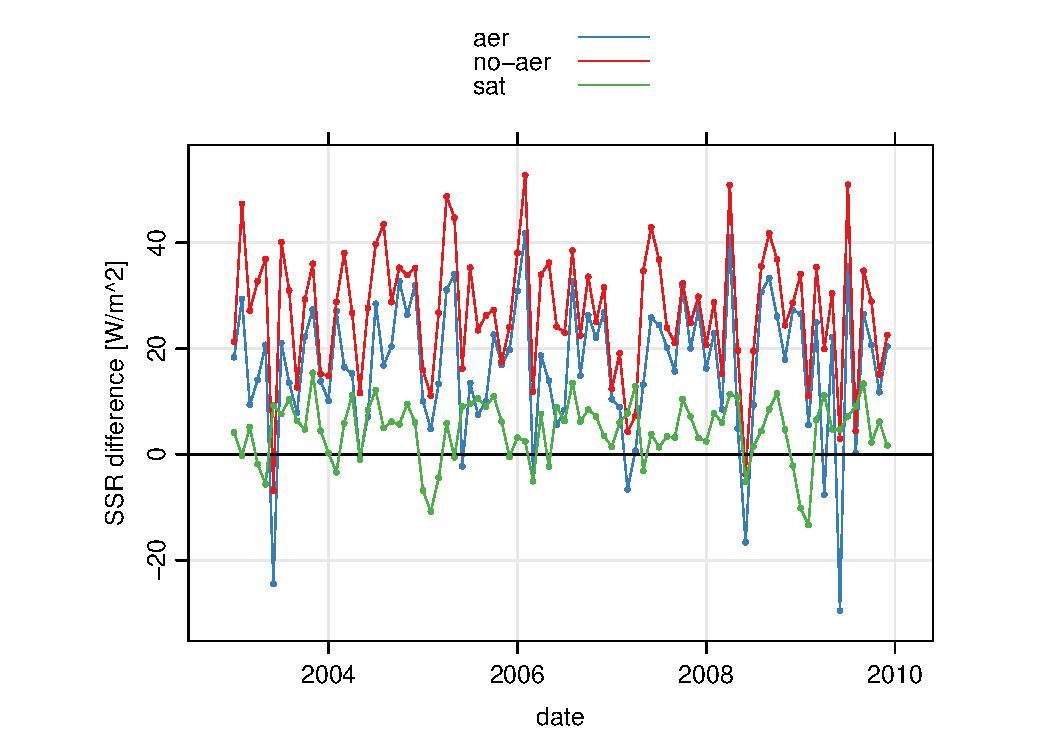
\includegraphics[width=1.2\textwidth]{figs/capitulo6/PayerneMesesDif.pdf}
    \caption{Payerne}
    \label{Payerne}
  \end{subfigure}
  %
    \centering\begin{subfigure}{0.4\textwidth}
    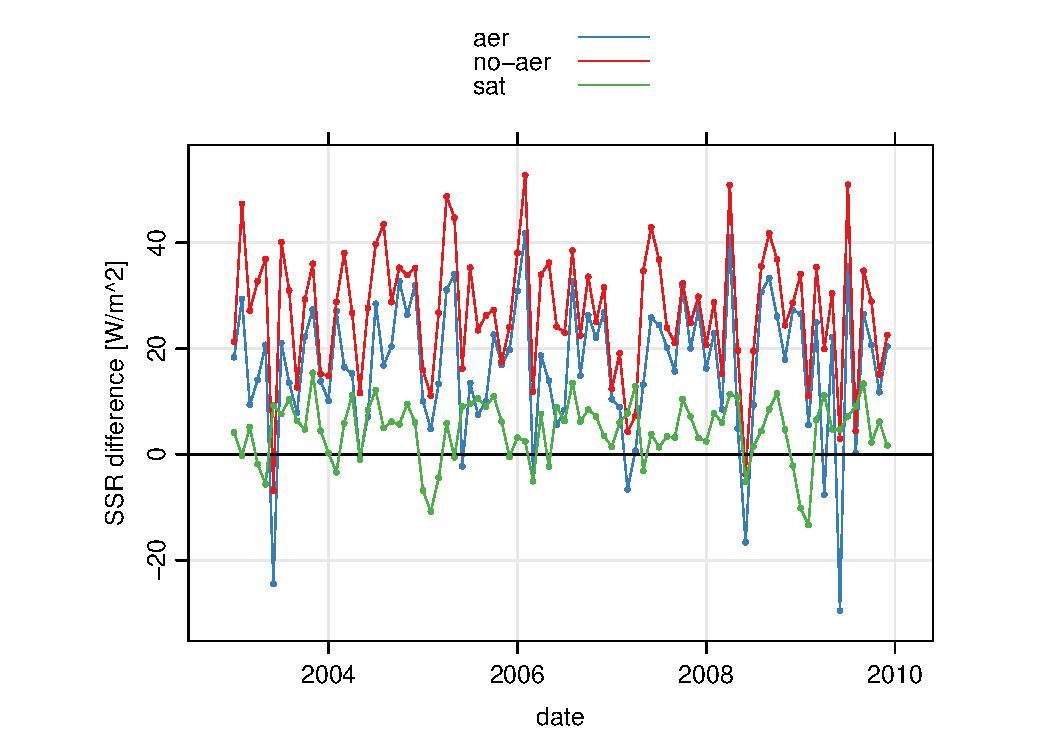
\includegraphics[width=1.2\textwidth]{figs/capitulo6/SedebokerMesesDif.pdf}
    \caption{Sede Boker}
    \label{fig:Sde Boker}
  \end{subfigure}
  \caption{Difference in SSR $\si{\watt\per\metro\squared}$ between both simulations and the satellite with respect to the data from BSRN stations (BSRN)}
    \label{fig:station}
\end{figure}

For the three stations, the satellite has better results than the simulations, although the error magnitude varies depending on the station. There is also a general improvement of the AER simulation against the NO-AER. Carpentras station is the one with lower bias with respect to the observed data \ref{Carpentras}. In the case of the Sede Boker station \ref{fig:Sde Boker}, there is a seasonal bias in the AER simulation. High negative differences appear from May to August, showing underestimation of the SSR in these months.

Several statistical measurements summarize the general performance of the SSR from the climate model and the PV simulations at each location and are reported in table \ref{RMSE_MAE_table}.

For the simulation of PV power output, the daily mean of PV production data averaged for each month is compared with simulated PV energy production at each power plant, using the three possibilities of SSR data as input: AER, NO-AER and SAT. For these simulations, in order to help with the visualization of the results a \textit{violin plot} is used to visualize the absolute error and its distribution.
For the Seville PV power plant, AER performs better than NO-AER and SAT simulations showing lower errors \ref{fig:figuraSEVILLA}. Besides, only AER has some negative errors, which means underestimation for some months, whereas the satellite and the NO-AER have only positive error values.

The median error for the AER simulation is less than 0.25 $\si{\kilo\watthour\per\kilo\wattpeak}$. Differences are concentrated around this value, which makes the distribution peaks around it in a narrow shape, although the range is wider due to higher values above 0.5 $\si{\kilo\watthour\per\kilo\wattpeak}$ that spread the distribution.

NO-AER simulation has a wider range of errors than AER and SAT, and a wider distribution. The satellite presents a median error close to 0.5 $\si{\kilo\watthour\per\kilo\wattpeak}$, as it could be expected from the evaluation and report of the CM-SAF dataset.

\begin{figure}[h!]
  \centering\begin{subfigure}{0.45\textwidth}
    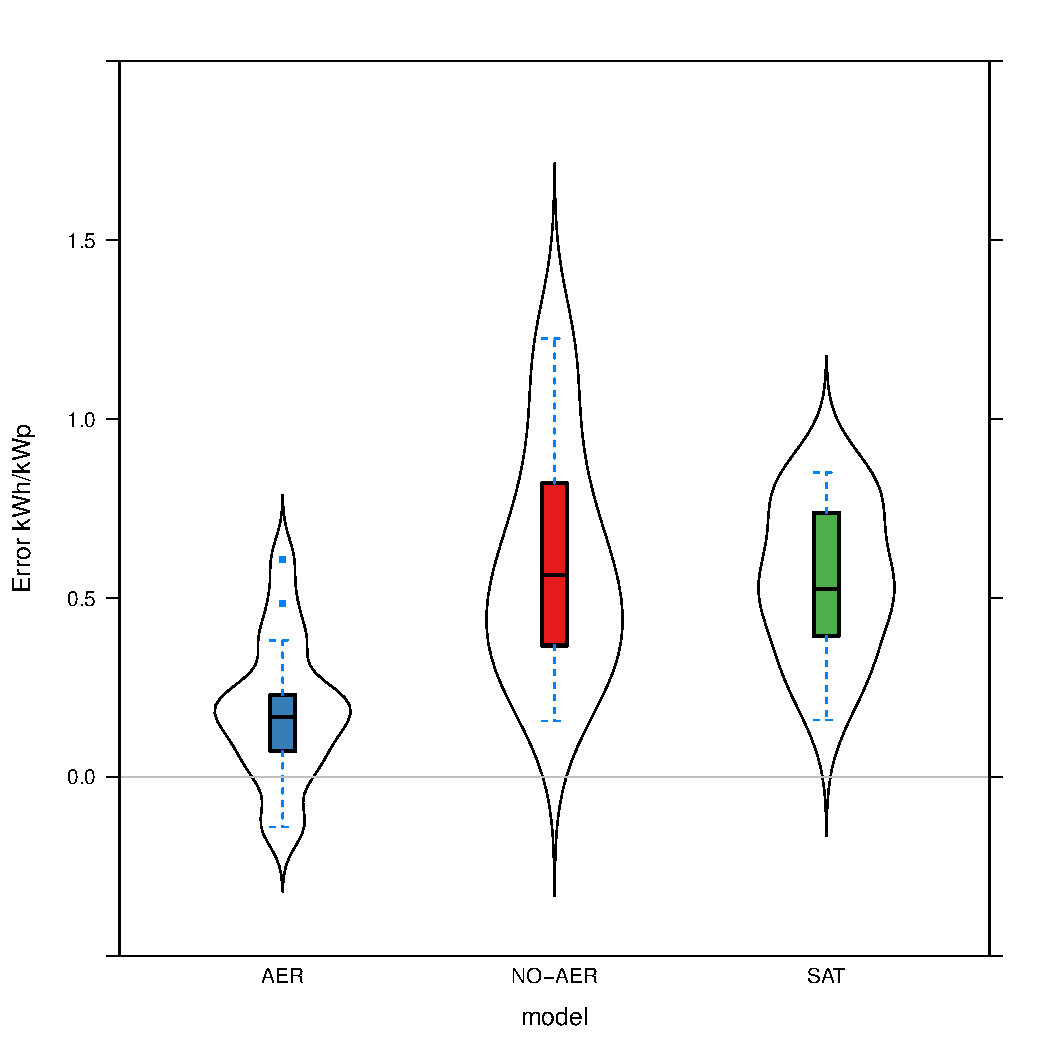
\includegraphics[width=1\textwidth]{figs/capitulo6/violinplorSeville.pdf}
    \caption{Seville}
    \label{fig:figuraSEVILLA}
  \end{subfigure}
  %
  \centering\begin{subfigure}{0.45\textwidth}
    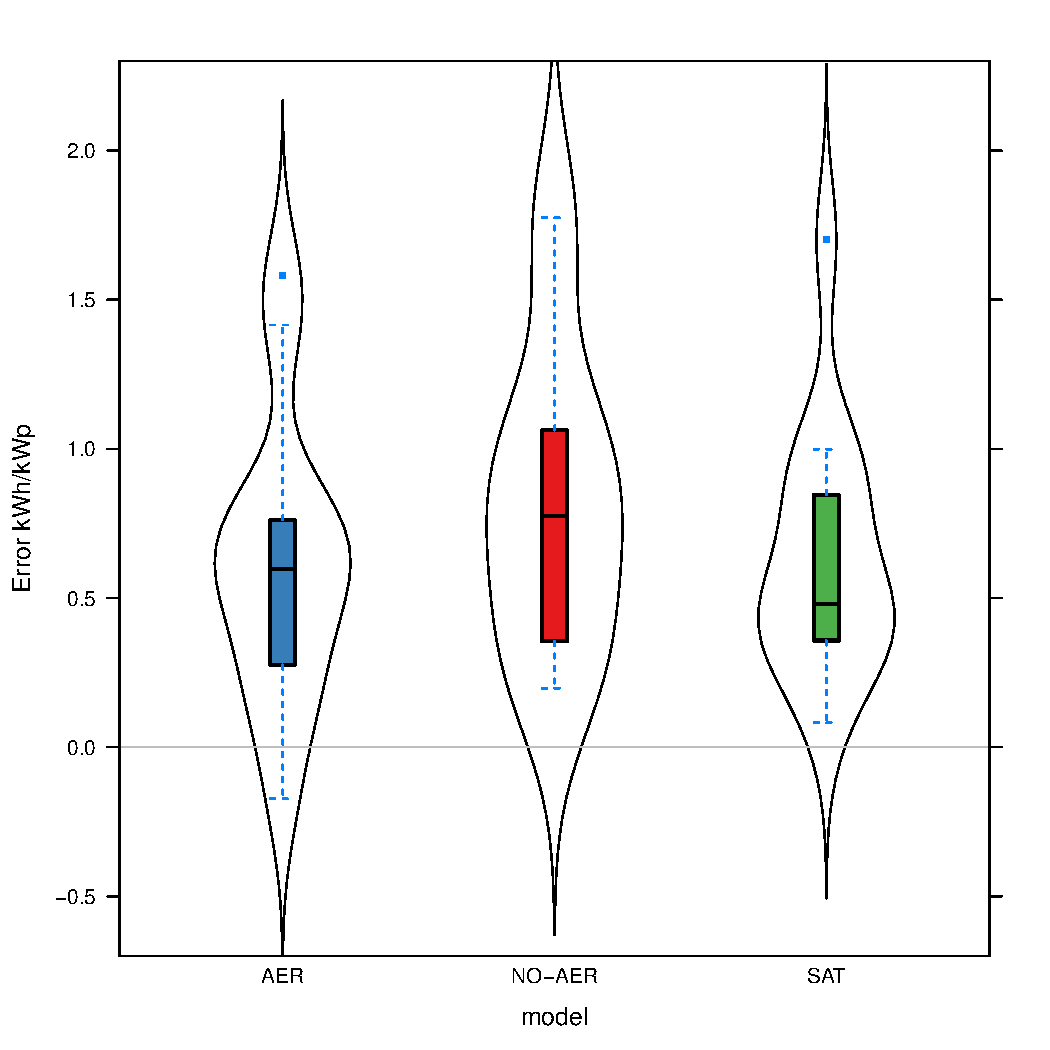
\includegraphics[width=1\textwidth]{figs/capitulo6/violinplotTarragona.pdf}
    \caption{Tarragona}
    \label{fig:violinTarragona}
  \end{subfigure}
  \caption{Distribution of differences in monthly mean of daily PV productivity $\si{\kilo\watthour\per\kilo\wattpeak}$ from Seville and Tarragona power plants and the simulated with the model, AER (blue) and NO-AER (red), and the satellite (green) in the same location. The period for Seville is from July 2007 to November 2008 and for Tarragona power plant from January 2003 to December 2005. The violin plot represents at the y-axis the probability density function of the variable, estimated with a kernel density estimation. Along this axis, the plot represents the shape of the variable distribution and it is duplicated by symmetry over an imaginary vertical axis to facilitate visualization. In this way it is easier to see not only statistical parameters represented in the boxplot, that it is also shown inside the violin, but also how the errors are distributed.}
    \label{violin}
  \end{figure}

\begin{table}[h!]
  \begin{tabular}{>{\raggedright}m{1.5cm}>{\raggedright}m{1.5cm}>{\raggedright}m{2cm}>{\raggedright}m{2cm}>{\raggedright}m{2cm}>{\raggedright}m{2cm}}
    \toprule 
    Location & \centering{Simulation} & \centering{RMSE} & \centering{MBE} &\centering{cor} &\centering{sd}\tabularnewline
    \midrule
    Seville & \centering{AER} & \centering{0.27} & \centering{0.18} & \centering{0.98} & \centering{1.34}
    \tabularnewline
    & \centering{NO-AER} & \centering{0.67} & \centering{0.60} & \centering{0.95} & \centering{1.29}
    \tabularnewline
    & \centering{SAT} & \centering{0.59} & \centering{0.55} & \centering{0.98} & \centering{1.45}
    \tabularnewline
   \midrule
    Tarragona & \centering{AER} & \centering{0.77} & \centering{0.61} & \centering{0.87} & \centering{1.21}
    \tabularnewline
    & \centering{NO-AER} & \centering{0.96} & \centering{0.82} & \centering{0.9} & \centering{1.29}
    \tabularnewline
    & \centering{SAT} & \centering{0.76} & \centering{0.64} & \centering{0.88} & \centering{1.13}
   \tabularnewline
   \midrule
  Payerne & \centering{AER} & \centering{21.21} & \centering{16.62} & \centering{0.97} & \centering{77.4}
  \tabularnewline
    & \centering{NO-AER} & \centering{29.70} & \centering{27.07} & \centering{0.98} & \centering{81.88}
  \tabularnewline                           
    & \centering{SAT} & \centering{7.36} & \centering{4.6} & \centering{0.99} & \centering{83.29}                         \tabularnewline
      \midrule
      Carpentras & \centering{AER} & \centering{16.59} & \centering{12.05} & \centering{0.98} & \centering{90.05}
  \tabularnewline
  & \centering{NO-AER} & \centering{27.26} & \centering{24.10} & \centering{0.99} & \centering{90.57}
  \tabularnewline
    & \centering{SAT} & \centering{6.38} & \centering{4.26} & \centering{1.00} & \centering{88.71}
 \tabularnewline
      \midrule
  Sede Boker & \centering{AER} & \centering{18.89} & \centering{8.17} & \centering{0.98} & \centering{62.83}
  \tabularnewline
  & \centering{NO-AER} & \centering{37.42} & \centering{35.63} & \centering{0.98} & \centering{76.06}
  \tabularnewline
    & \centering{SAT} & \centering{12.00} & \centering{10.27} & \centering{0.99} & \centering{77.62}
 \tabularnewline
 \bottomrule
  \end{tabular}
  \caption{Values for the root mean squared error (RMSE), mean bias error (MBE), temporal correlation (cor) and standard deviation (sd) for the simulated PV production in Seville power plant and Tarragona power plant compared with the final productivity data measured $\si{\kilo\watthour\per\kilo\wattpeak}$ and the SSR from the climate model simulations and the satellite in comparison with the SSR from BSRN stations $\si{\watt\per\metro\squared}$}
  \label{RMSE_MAE_table}
\end{table}

The Tarragona PV power plant presents larger errors. The SAT has slightly better performance than AER and the improvement with respect to NO-AER can be observed in both cases. 

AER simulation's median error is 0.60 $\si{\kilo\watthour\per\kilo\wattpeak}$ and NO-AER simulation error has larger values, the median is 0.77  $\si{\kilo\watthour\per\kilo\wattpeak}$. The SAT error has lower median value: 0.48  $\si{\kilo\watthour\per\kilo\wattpeak}$.

It can be also appreciated in figure \ref{fig:violinTarragona} that there are two months in the simulations where errors are specially large. As these values are clear outliers, it might be that some maintenance activities in the plant are the cause of the lower energy output than expected, which would explain the larger errors in those months.  

The added value of including aerosols in climate simulations for the estimation of PV production is clearly illustrated by our results. The model using climate simulations with a good aerosols representation could be locally as good as the satellite, at least at the location of the PV power plants used (despite of its biases in some areas). The satellite product has revealed itself also as a good dataset, either for SSR (seen in the evaluation with BSRN stations) and for the PV production estimation.

\subsection{Regional scale}

The regions defined in figure \ref{fig:mapapral} are the same areas selected in \cite{Nabat2014}, and the acronyms used in this section are also in the figure. The difference between simulations and satellite data in annual terms is represented in figure \ref{fig:figura4}. The improvement of the simulation including aerosols is noticeable for every region. It can be appreciated also that there are some weak changes in the interannual variability of the bias due to aerosols inclusion, like in the BISL area, AFRE region in 2009 or AFRW.

Western (EURW) and Southern Europe (EURS) have the lowest biases in SSR, as well as eastern Africa (AFRE) and the South of British Islands (BISL). Negative biases only appear for Africa and they could be due to the fact that in some cases the annual amount of aerosols is overestimated, or due to the optical properties of the aerosols in the model. The rest of the areas have positive biases, probably due to an underestimation of the cloud cover in the model \citep{Nabat2014}. The east side of the domain shows a higher bias (NEEUR), although it is clear that the addition of aerosols improves the representation of SSR. 

\begin{figure}[h!]
\centering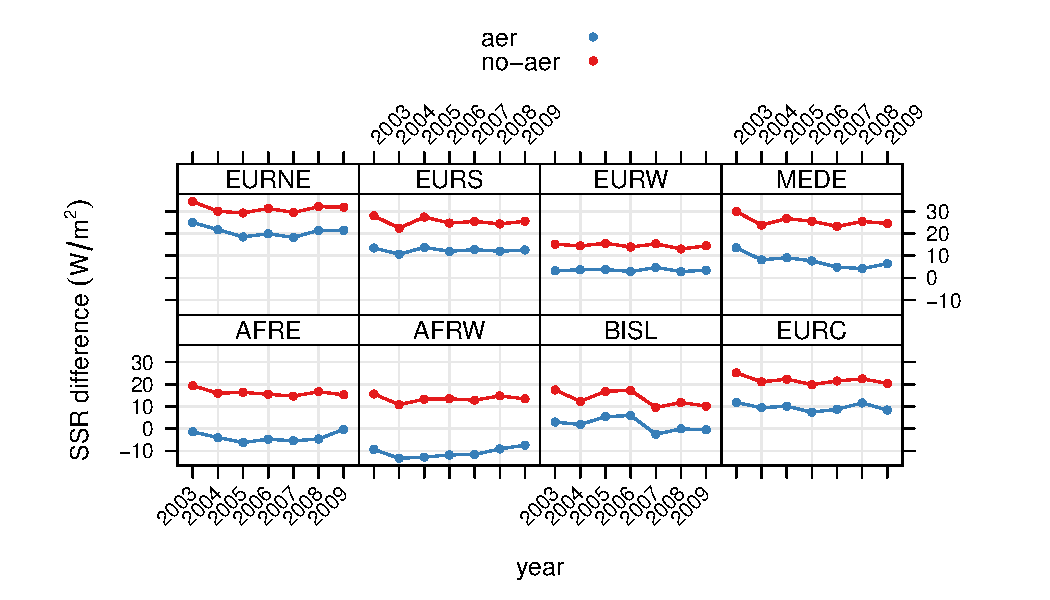
\includegraphics[width=1\textwidth]{figs/capitulo6/dif_model_sat_zonas.pdf}
\caption{Difference in shortwave solar irradiation, SSR $\si{\watt\per\metro\squared}$, between simulations and the satellite aggregated by areas defined in figure \ref{fig:mapapral} in the period 2003-2009.}
\label{fig:figura4}
\end{figure}

In order to calculate the impact on photovolaic production, shortwave solar irradiation, SSR, from the climate model simulations and the satellite dataset is used as an input of the photovoltaic model. For a fixed typology of the panels, the difference between simulations with respect to the satellite dataset as input, in the mean of daily productivity for each month, is represented in figure \ref{fig:ciclosFixed}. The productivity is defined as the energy production per unit of power installed  $\si{\kilo\wattpeak}$.

In general, The NO-AER simulation gives more production than the AER and the satellite, overestimating the PV power potential. Climate model simulations, AER and NO-AER, differ more from satellite PV production output in winter months, whereas in summer months, AER and satellite are close to each other, except form the EURNE region. This area is the most biased area of the model in comparison with the satellite, perhaps due to a bias in the cloud cover.

The regions from North Africa, AFRE and AFRW, are slightly different from the rest with a roughly constant bias curve of the the annual cycle, therefore the difference in PV production between summer and winter months is lower due to the mean latitude of the area. Besides, for these areas, the AER simulations give in summer month lower PV production values than the SAT and the NO-AER, which is not the case in the rest of the regions.

The EURS area is the one with largest amplitude between winter and summer months. For April and May, the AER simulations has small difference with the satellite simulation.

\begin{figure}[h!]
\centering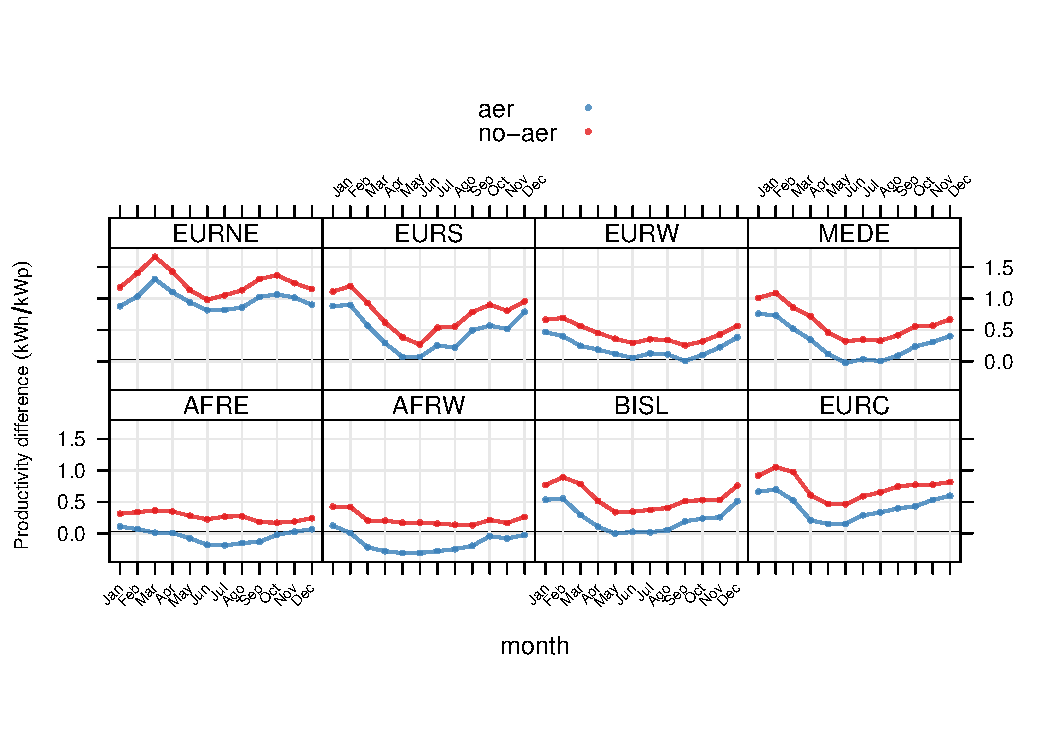
\includegraphics[width=1\textwidth]{figs/capitulo6/diferencia_mesesFIXED.pdf}
\caption{Annual cycle of daily energy productivity  $\si{\kilo\watthour\per\kilo\wattpeak}$ differences by area for the AER simulation and NO-AER simulation with respect to the satellite as inputs of the PV model, considering fixed panels.}
\label{fig:ciclosFixed}\end{figure}

\subsection{Impact of aerosols by tracking type}

\subsubsection{Mean behavior. Period 2003-2009}

In addition to the absolute difference in PV productivity between AER and NO-AER, the relative difference between simulations is presented in this section, showing the relative impact in each case. It allows us to contextualize the loss with respect of the potential of the place.

The difference in yearly PV production between both simulations, for every type of tracking panel, is represented in figure \ref{fig:diferenciaYm}. The spatial pattern shows areas where the aerosols affect more the shortwave solar radiation. Central Europe, Po Valley and the South of the domain, along the African continent coast, are the areas where the differences are more noticeable.

For the fixed panels, the differences are around -150 $\si{\kilo\watthour\per\kilo\wattpeak}$ for some of these areas in annual terms and reaching -200 $\si{\kilo\watthour\per\kilo\wattpeak}$ in the Po Valley, Syria, Iraq and between Algeria and Tunisia.

When the two other tracking systems are considered, the difference between both simulations increases, with values of -300 $\si{\kilo\watthour\per\kilo\wattpeak}$ for the two-axes type over the most affected areas and even higher values like in the south of Turkey. These results are consistent due to the fact that the two-axes and the one-axis tracking systems are more efficient systems to give energy to the generator.

\begin{figure}[h!]
  \centering\begin{subfigure}{1\textwidth}
    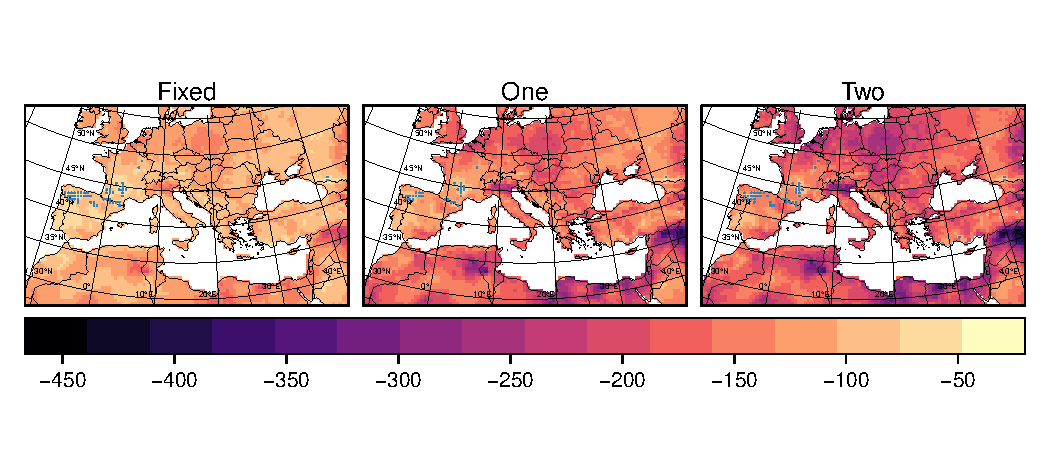
\includegraphics[width=1\textwidth]{figs/capitulo6/dif_aer_no_all_Ym20032009SIGt.pdf}
    \caption{}
    \label{fig:diferenciaYm}
  \end{subfigure}
  %
  \centering\begin{subfigure}{1\textwidth}
    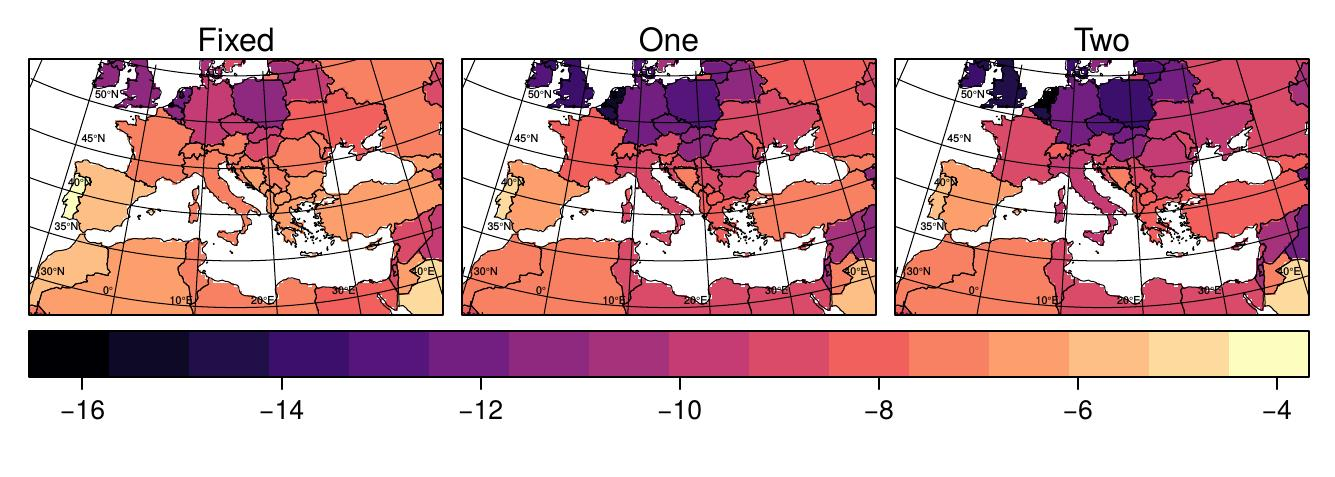
\includegraphics[width=1\textwidth]{figs/capitulo6/byCountry.jpeg}%year_all_bycountry.pdf}%{figs/RelDif_aer_no_all_Ym20032009.pdf}
    \caption{}
    \label{fig:diferenciasRel}
  \end{subfigure}
  %
  \caption{Differences in PV yearly productivity: (a) absolute $\si{\kilo\watthour\per\kilo\wattpeak}$, (b) relative averaged by country (\%); for the period 2003-2009 between AER and NO-AER and for the three different types of tracking. For he non-significant differences, calculated with a 't-test', a point is overplotted for (a)}
\end{figure}

The results of the country averages for the annual productivity are shown in figure \ref{fig:diferenciasRel}. It is shown that the aerosols impact range from $-4\%$ to the PV production to $-16\%$. It can be seen that from the fixed panels to the one-axis, and then to the two-axes tracking type, there is an increase in the productivity losses that is more noticeable in Central Europe, like in Belgium-The Netherlands.

Germany, that have installed a high amount of PV capacity, is affected with values around $-10\%$ of loss for fixed system and more than $-12\%$ for the one-axis and two-axes panels. Thus, some countries with high PV production have moderate losses due to aerosols in relative terms. For countries in the west and south of the domain like Portugal, Spain, Morocco, Jordanian or the extension of Saudi Arabia included in the domain, the relative amount of energy loss is smaller due to its high potential, with differences between $-5\%$ and $-6\%$ for fixed panels and reaching $-8\%$ in some cases for the other types of tracking systems.

\subsubsection{Seasonal cycle}

\begin{figure}[h!]
  \centering
  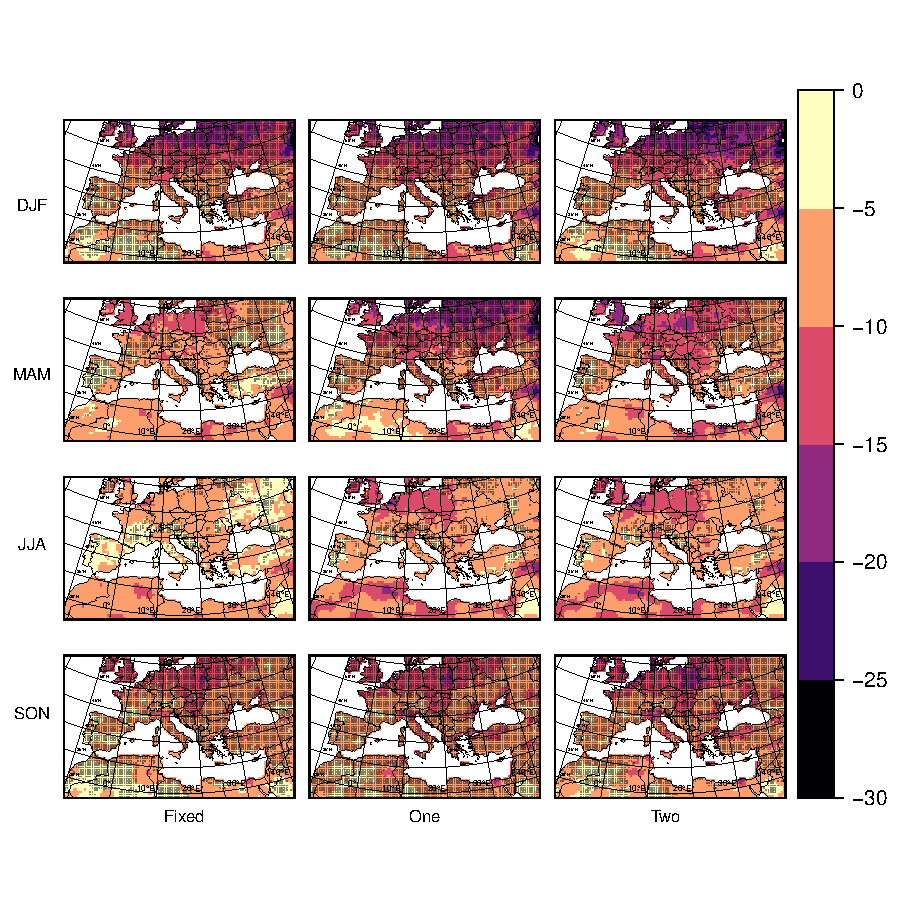
\includegraphics[width=1\textwidth]{figs/capitulo6/RelDif_aer_no_all20032009SIGt.pdf}
\caption{Relative difference (\%) in seasonal PV productivity between both simulation for all type of panels. For the non-significant absolute differences, calculated with a 't-test', a dot is overplotted.}
\label{mapas}
\end{figure}

In seasonal terms spring (MAM) and summer months (JJA) show statistically significant values of the PV productivity difference. For winter (DJF) and Autumn (SON), there are few significant areas, mostly located at the south of the domain, in the African continent. An exception can be found for fixed panels in winter, with significant zones in Europe with values above $-10\%$, like the Po Valley or British Islands. 

The spatial pattern for the spring season shows higher values in Central-Europe, in specific countries like Poland, Belgium and The Netherlands, or British Islands, and in northern parts of Syria and Iraq. Maximum values in these areas, range from an impact higher than $-10\%$ for fixed panels to around $-15\%$ for the two axes tracking type. Almost the whole African part of the domain shows significant differences, with impact values above $-5\%$ and local values reaching more than $-10\%$ between Algerya and Tunisia and in areas of Lybia or Egypt. 

Summer months have higher loads of aerosols over the Mediterranean. For fixed panels, only a few areas in north Africa, Middle East and north-western Europe show values with a loss higher than $-10\%$. One-axis tracking enlarge the extension of areas with a decrease higher than $10\%$ and some areas with more than $-15\%$ appear in Belgium and The Netherlands, Algeria and Syria-Iraq border. Also some smaller areas appear with PV production losses above $-15\%$ within the above mentioned areas. Between the one-axis and the two-axes tracking type, there are no substantial differences in the spatial pattern but maximum values reach in these cases $-17\%$ to $-20\%$ in the same areas.

Significance is not clearly linked to the magnitude of the relative difference in productivity. High relative differences in DJF and SON in central and northern Europe are not significant, due to the high climate variability in these areas and seasons, whereas lower relative differences in spring in Africa and in summer in southern and eastern Europe are mostly significant. The fact that JJA changes are significant over most of the domain explains the statistical significance of most yearly differences (figure \ref{fig:diferenciaYm}), due to the high contribution of summer to the yearly production and yearly interannual variability (see e.g. \cite{Gil2015}).


\subsection{Long-term trends. Period 1980-2012}

The impact of long term trends of solar shortwave on PV production can be illustrated with the results of the simulations of the brightening period over Europe. The simulation including the aerosols dataset, NAB13, and the decreasing trend in sulfur aerosols, TREND, is able to reproduce the observed positive trend in SSR \citep{Nabat2014}.

As a compromise between the lifetime of a PV plant and the length of the simulation, two 15-year periods (at the beginning and end of the simulated period) are evaluated as a proxy for a PV project and the potential amount of energy that can be obtained during such a project. A fixed system is selected for the panels.

The relative difference between the accumulated energy obtained by a 15-year project between 1997-2012 and energy obtained by a 15-year project between 1980-1995 can be seen in figure \ref{fig:trends}.

\begin{figure}[h!]
  \centering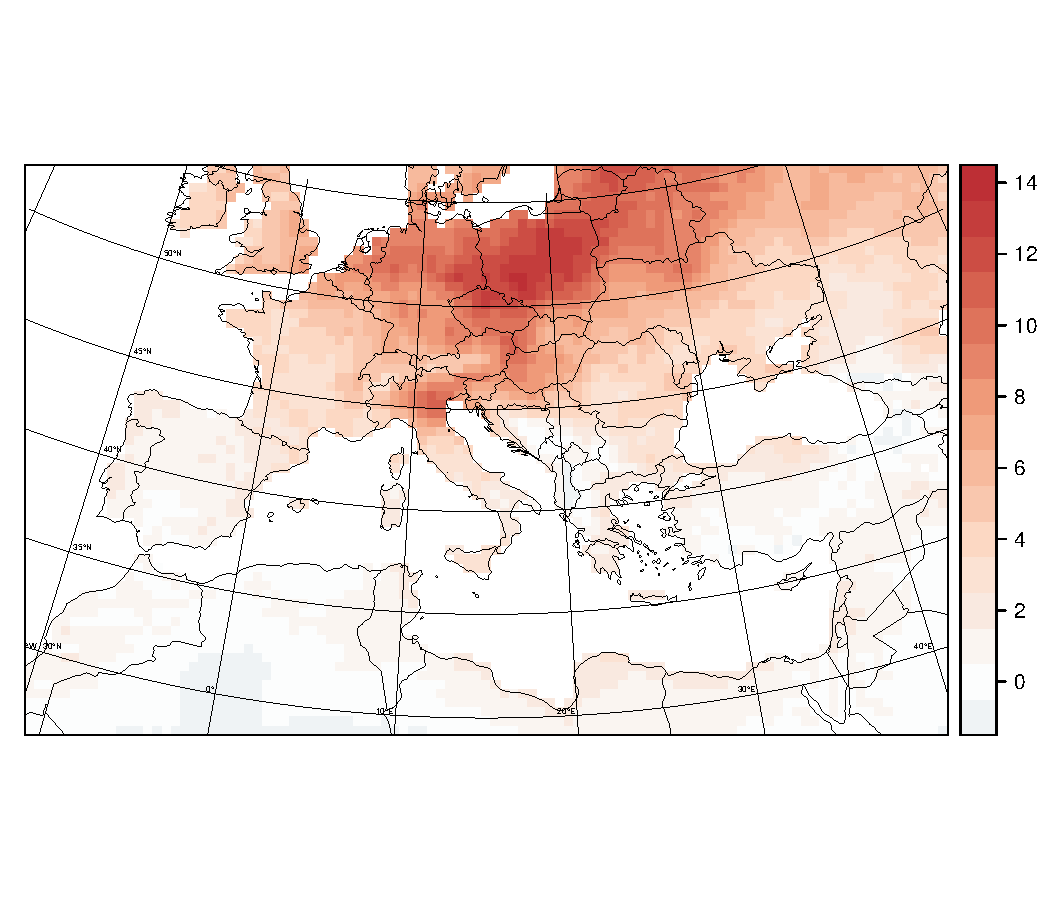
\includegraphics[width=0.7\textwidth]{figs/capitulo6/DifferencesRelativesinPVtciclo15.pdf}
\caption{Relative difference in PV yearly productivity $[\%]$ accumulated for a 15-year period at the end and the beginning of the period: 1980-1994/1998-2012}
\label{fig:trends}
\end{figure}

In Central-Europe the differences in the energy obtained are higher, due to the fact that it is the region where anthropogenic aerosols decrease more. Accumulated over 15 years, an increase higher than 2000 $\si{\kilo\watthour\per\kilo\wattpeak}$ is found for this area. It means that about 10-14 $\%$ more energy can be produced in the lifetime of a PV plant at the end of the period.

These results highlight the impact that environmental policies could have on the PV energy production, showing that anthropogenic aerosols are able to reduce potential PV power of a project significantly. It also illustrates that future evolution of regional anthropogenic aerosols load is likely to influence expected PV production on a given site on the lifetime of a PV plant.

\section{Discussion}
\subsection{Limitations}

The coarse resolution of climate models and their bias in some variables, especially in cloud cover, makes difficult their application for solar resource assessment at local scale in most areas. However, the RCM will evolve to finer resolution and besides, the use of climate models is mandatory for taking into account future climate evolution. They are also relevant tools to perform sensitivity tests allowing to disentangle the driving factors of the resource variability such as aerosols. 

A multi-model approach would be necessary to obtain a more robust answer applying the same methodology to more models but, up to now, aerosols are poorly considered in many RCM, which does not allow that type of study considering actual simulations. 

For the limitations in the PV model, it is important to notice that in the decomposition of SSR and the transposition to the tilted panels, some empirical relationships are used. If components of solar radiation were an output of the RCM, the additional steps for decomposition could be avoided.

It could also be pointed that the spectral decomposition of the SSR reaching the panels would give a better input in order to calculate spectral losses of the PV modules, although for periods longer than a day the spectral effects become less significant \citep{Martin1999}.

In the optical losses, deposition of dust over the generator surface is approximated in the assessment but could be underestimated in desert areas because it is not spatially modeled. That could mean a higher drop in transmittance and final energy production.

The time-scale is also important for the AOD representation. Several processes involving aerosols in the atmosphere are in day to weeks time-scales. We have used a realistic interannual dataset of the AOD that improves the state-of the art used in climate modeling but next studies should go further with an improvement in the aerosols representation. This will include a prognostic scheme of aerosols that allows to study finer time-scales and future scenarios, through a fully-coupled and fully-interactive aerosol-climate model. 
  

\subsection{Implications for the climate services dedicated to the energy sector }

The results show the necessity of considering aerosols in climate simulations used to deliver energy-related climate services. The inclusion of spatio-temporal variability of aerosols in RCMs may change the current estimates of future PV production over Europe \citep{Jerez2015}. An accurate ensemble of models is essential for bridging the gap between services providers and potential users considering that some of the discrepancies between model simulations could come from the aerosols inclusion.

\subsection{PV production data issue}

The scarcity of real power data at PV plant sites is an important issue that has to be overcome in order to improve research in the fields of PV forecasting, climate services or energy modeling. The potential synergies between research institutions and different stakeholders of the energy sector will enhance the PV integration, the management and planning operations as well as the efficiency of the overall system and its development. Not only production data is needed, but also, accurate metadata will be extremely important in order to integrate into the modeling chain important factors such as: days of maintenance activities, cleaning-panel days, installed capacity, electrical characteristics of the PV power plant, among others.

\section{Conclusions}

Two main questions are addressed in this paper: first, the evaluation of the capacity of an RCM to produce reliable estimations of PV production over the Mediterranean area. Secondly, the role of aerosols in PV production using sensitivity tests performed with the RCM. 

It is demonstrated that the use of a RCM as input of a photovoltaic production model is able to reproduce real PV data accurately at monthly time scales for two locations at the domain. Besides, the added value of including aerosols in the simulations is observed over the whole area as the simulation with aerosols shows less bias in SSR than the simulations without aerosols and it is close to the simulated PV using the satellite dataset accross the whole area. 

The results show that the most impacted areas are (with some exceptions) mostly in central Europe, where the lower resource amount in combination with the influence of aerosols gives a significant reduction in potential electricity production. For the annual averaged by country productivity, relative differences are around $-12\%$ for fixed typologies and are seen over Central Europe (Poland and The Netherlands). Differences increase from one axis typology to the two-axes, reaching around $-16\%$ between both simulations in Belgium and around $-13\%$ and $-14\%$ in many countries. In seasonal terms, the loss can reach values of $-20\%$ in some areas for summer months.

In the multi-decadal simulation 1980-2012 a noticeable increase in productivity has been obtained in central Europe as a result of the decreasing trend of anthropogenic aerosols observed from the end of the eighties. This trend has been associated with pollution control measures as well as economic crisis in Western Europe. This result has implications beyond the domain of this study: highly polluted countries like India and China could obtain an increase in PV productivity if pollution control policies are effectively implemented.

The non-negligible impact of aerosols on PV production in the area suggests that the inclusion of aerosols in future scenarios is necessary for solar energy assessment.

\chapter{Future projections of solar resource for photovoltaic applications}

\begin{abstract}

  With the ongoing energy transition, the evolution of renewable energy resources under different climate change scenarios is key for the investors and stakeholders of the energy industry. The possibility of changes in the actual conditions for the operating plants and the projected resources can vary the financial frame of the projects.\\
  
  Although climate models give a robust answer in terms of global warming and other important climate variables, they dissagree in the projected changes of solar resource over Europe. Whereas global climate models, GCM, present a clear positive signal around the mid of XXI century, regional climate models, some studies show a negative anomaly for the same period in RCMs.\\
  
  In this chapter we try to explain the reasons behind the different behaviour focusing on the representation of aerosols in the scenario simulations. We use regional climate models from the EURO-CORDEX project and we focus on the RCP8.5.\\
  
  A fairly pairwise comparison show that regional climate models that include evolving aerosols for the scenarios reverse the sign of the signal in the shortwave solar radiation over Europe.\\
  
  We analyse total cloud cover in the regional models simulations and it is not find a clear relationship between the models with aerosols and the anomaly in cloud cover.\\
  
  Due to the clear relationship between sortwave solar radiation anomaly and aerosols evolution, it is necessary to prepare an experiment that is able to give a robust answer in the role of aerosols in terms of shortwave solar radiation projections, which means, that is able to narrow down the uncertainties.\\

  In terms of photovoltaic (PV) potential it has been shown that for RCM with evolving aerosols countries in Central-Europe has a positive anomaly, in contrast with the rest of the RCMs projections. Those RCMs projections including evolving aerosols agree with GCM projections. This result reveals the impact that the representation of aerosols has in the projections of PV potential for the climate services.\\ 
\end{abstract}

\section{Introduction}

    The generalized increase in the photovoltaic installed capacity in last decades demands the delatiled study of spatio-temporal features of solar resource.\\

  Due to the link between solar energy production and atmospheric variables, there is an increasing concern motivated by the availability of resources under climate change scenarios. Due to that, climate modelling is a key tool to evaluate future energy potential despite of some constrains like its low spatial resolution or cloudiness representation.\\
  
   Although variability of solar radiation are mainly due to changes in cloudiness, in clear days other constituents of the atmosphere, mostly aerosols, decrease the amount of energy reaching the generator surface[ref]. Because of its geographical situation, the Euro-Mediterranean area is one of the most influenced areas by natural and anthropogenic aerosols comming from different sources, affecting the spatio-temporal distribution of solar resource.[ref]\\

   Different CMIP5 simulations with different GCMs have been evaluated to assess the photovoltaic potential under climate change conditions (wild et al.) and projecting an increase over Europe. However, later studies using regional climate models (Jerez et al. Bartok) have shown an opposite behaviour, an overall decrease in shortwave solar radiation and photovoltaic potential in the same area.\\

   The added value of regional climate modeling against global simulations lies on the better representation of local features that can not be solved with coarser models. However, the increase in resolution has lead to a simplification of other processes in order to not compromise the computational time. Many regional climate simulations have been done using a very simplistic representation of aerosols content (nabat) and they do not include an evolution of aerosols in future projections.\\
   
   In this work we analyse the projections of photovoltaic potential over Europe for the RCP8.5 scenario using regional climate models simulations from EURO-CORDEX initiative. We classify diferent simulations atending to the aerosol representation in the model and its driving global climate model.\\

   Section \ref{Climate data} describes the regional models and simulations used in the study and in section \ref{Aerosols} there is a descrioption of the datasets used by them.  In section 3 the the main results are explained and a discussion section followed.\\

\section{Climate data}

\subsection{EURO-CORDEX}

The EURO-CORDEX (Jacob et. al 2014) initiative started as a 'branch' from the Coordinated Regional Climate Downscalling, CORDEX, whose aim is to provide regional climate simulations in different domains. EURO-CORDEX develops climate projections focused on the European continent at different horizontal resolutions (0.44º, 0.11º). These simulations are driven by different CMIP5 GCMs (Taylor et. al 2012).\\

In table 1 there is the information about the aerosols datasets included in the EURO-CORDEX RCMs. It can be observed that only two RCMs include time-evolution of aerosols: RACMO22e and ALADIN5.3. Each of these RCMs have a different dataset of aerosols for projections. Whereas ALADIN5.3 select the Szopa dataset, RACMO22E uses the CAM inventory (Lamarqué et al).\\ 

The choice for the different simulations in this chapter has followed the next 'pairwise' principle: firstly, RCMs simulations from the EURO-CORDEX database including time evolving scenarios of aerosols are selected. Then, a family of RCMs simulations driven by the same GCMs is constructed around it. Following these steps, we will obtain several groups of RCMs simulations where each one will be called 'family' with the same driven GCM and with only one simulation including aerosols scenarios. Besides, we consider only the RCP8.5 because changes in SSR will be more noticeable and differences between simulations easily detected.\\ 

%**La tabla de la descripción de aerosoles de bartok de los GCM se puede referenciar y hacer la de aerosoles de EURO-CORDEX (o de los modelos que yo utilizo?)

\begin{table}
\caption{\label{tb:families}RCMs from EURO-CORDEX grouped by the CMIP5 GCMs drivers generating the 3 families of simulations studied.}
\footnotesize
\begin{tabular}{>{\raggedrigth}m{3cm}>{\raggedright}m{3cm}>{\raggedright}m{3cm}}
\toprule 
CMIP5 GCM & Institution  & RCM  \tabularnewline
\midrule
 CNRM-CM5 & CNRM & ALADIN5.3 \tabularnewline
&CLMcom&CCLM4-8-17\tabularnewline 
&SMHI&RCA4\tabularnewline
\midrule  
ICHEC-EC-EARTH&KNMI&RACMO\tabularnewline
&CLMcom&CCLM4-8-17\tabularnewline
&SMHI&RCA4\tabularnewline
%\midrule  
%HadGEM2-ES&KNMI&RACMO\tabularnewline
%&CLMcom&CCLM4-8-17\tabularnewline
%&SMHI&RCA4\tabularnewline  
\bottomrule
%  \br
\end{tabular}\\
%$^{a}$UK spelling is required; $^{b}$MSC classification numbers are required; $^{c}$titles of articles are required in journal references; $^{d}$Harvard-style references must be used (see section \ref{except}); $^{e}$final page numbers of articles are required in journal references.
\end{table}
\normalsize

\subsection{Aerosols datasets}

Different datasets are used for the RCMs simulations. Only ALADIN5.3 and RACMO22E include in their scenario runs evolving aerosols. For ALADIN5.3 the Szopa  ?? No tengo claro si incluir esta sección. De hacerlo, ¿describo todos los dataset? ¿únicamente los que utilizan los modelos que tienen evolución temporal?


\begin{table}
\caption{\label{tb:families}RCMs from EURO-CORDEX and aerosols description.}
\footnotesize
\begin{tabular}{>{\raggedrigth}m{1.3cm}>{\raggedright}m{1.3cm}|>{\raggedright}m{2.2cm}>{\raggedright}m{2.2cm}>{\raggedright}m{2cm}}
\toprule 
Institution  & RCM & description & classes & scenarios \tabularnewline
\midrule
CNRM & ALADIN5.3 & Climatology. Szopa 2013 & 5 classes: sea salt, sulfate,black carbon, desert dust,organic carbon.& evolve with RCP \tabularnewline
CLMcom&CCLM4-8-17& Climatology. Tanré 1984 & 4 classes: sea, land, desert, urban.& no evolution\tabularnewline 
SMHI&RCA4& Parametrization in radiation fluxes & Single integrated class.& no evolution \tabularnewline
KNMI&RACMO&CAM inventory, Lamarque 2010 & 6 classes: sulfate, organic matter, desert dust, sea salt,stratospheric aerosols, volcanic & evolve with RCP\tabularnewline
\bottomrule
%  \br
\end{tabular}\\
%$^{a}$UK spelling is required; $^{b}$MSC classification numbers are required; $^{c}$titles of articles are required in journal references; $^{d}$Harvard-style references must be used (see section \ref{except}); $^{e}$final page numbers of articles are required in journal references.
\end{table}
\normalsize

\section{Methods}

\subsection{Spatial analysis}

In order to analyse the spatial behaviour of shortwave solar radiation, SSR, it is calculated the mean yearly anomaly for the period 2021-2050 with respect to the reference period 1971-2000. The yearly anomaly is obtained only for summer montths, June, July and Augoust, JJA, which correspond to the season when the AOD (aerosols optical depth) is higher over Europe and the Mediterranean area.\\

The 2021-2050 period has been selected because of two reasons: in the mid-century the effects of global warming are not still very remarkable among the simulations, which could help to better detect the impact of including evolving aerosols. On the other hand, the PV power plants operating during 2021-2050 are the ones that will be planned shortly, so the results are important for the industry.\\

As an important driver of the variability of SSR the same procedure is applied to the total cloud cover variable, CLT. This allow us to know if there is correlation between both anomalies and how this correlation behaves for models including aerosols.\\

\subsection{PV potential}

In order to obtain a projection of the photovoltaic productivity over Europe under climate change scenarios, a modeling chain approach is considered. Shortwave solar radiation from different climate simulations is used as an input of a photovoltaic model that will give an estimation of the power output. The complete process is explained in chapter 4.\\

The two steps followed in the modeling process of the photovoltaic output are: first, it is necessary to get solar irradiation that reach solar cells, after that the electrical performance of the system is modeled.\\

The process is described in \ref{cha:methods}. In this case, monthly means of daily solar irradiation are used for the decomposition and transformation to the plane of array. Correlation equations between de diffuse fraction and the clearness index described by Page are applied. After the decomposition, the components are transposed to the plane-of-array using equations 4.7 and 4.8.\\   

\section{Results}

\subsection{Anomalies of SSR and CLT}

The anual mean anomaly of the period 2021-2050 for summer months (JJA) with respect to the reference period 1971-2000 is represented in figures \ref{fig:anomalySSR} and \ref{fig:anomalyCLT} first for shortwave solar irradiation, SSR, and then for total cloud cover, CLT.\\

\begin{figure}[h!]
\centering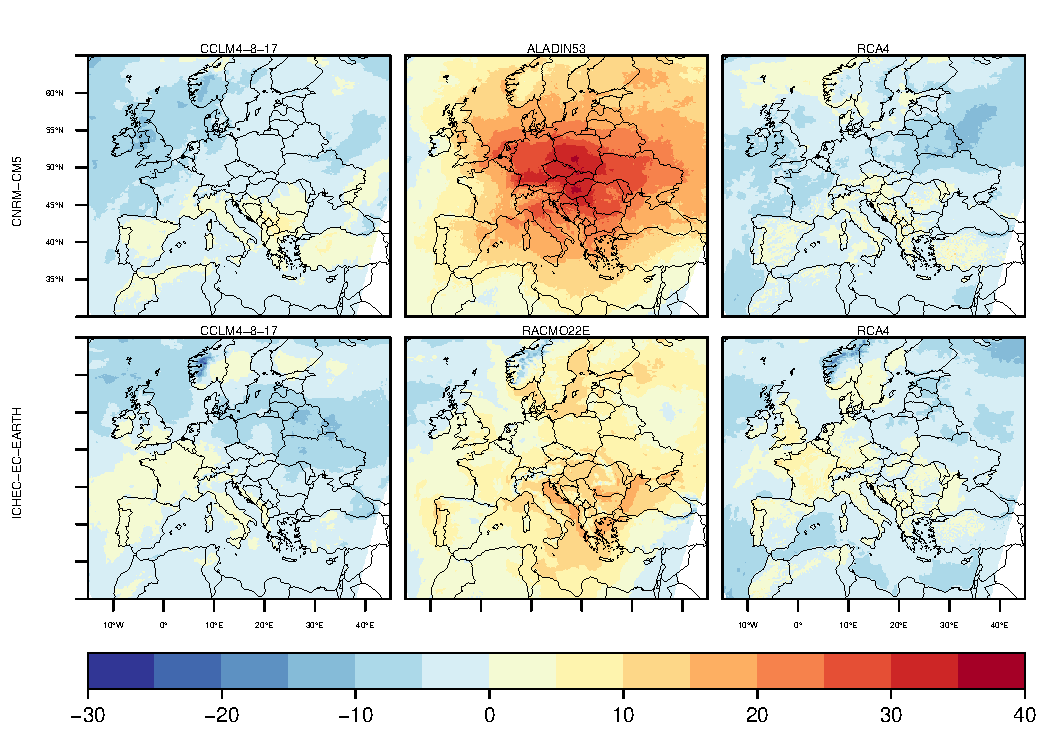
\includegraphics[width=1\textwidth]{figs/capitulo7/ANOMALIAS_JJA_SSR_2050-2021_r12.pdf}
\caption{}
\label{fig:anomalySSR}
\end{figure}

Annual mean anomaly for summer months shows an increase in Europe, more relevant in Central-Europe, for climate models with evolving aerosols in scenarios (ALADIN5.3 AND RACMO22E) although there are differences in the magnitude of the changes. ALADIN5.3 presents highest anomaly in the mentioned area, which correlates with the negative anomaly and spatial pattern of aod of this model, as can be seen in figure \ref{fig:anomalyAOD}. For RACMO, the aod anomaly has similar spatial pattern but the magnitude is sligthly smaller. The the projected SSR anomalies in RACMO are positive for a large area among the domain altought they don not reach the higher value of the ALADIN5.3. Mean values for the whole domain are positive for ALADIN (7.15 $W/m^2$) and RACMO (2.60 $W/m^2$) and negative for the others.\\

The rest of the RCMs from the first and second family presents a similar anomaly in SSR among them, with a sligthly decrease in SSR with the exception of southern and western Europe that shows a small increase.\\

With respect to the CLT anomalies it is noteworthy that they are not able to explain anomalies in SSR. For both families and the whole group of simulations the anomaly in CLT is close to cero as it can be seen in table \ref{}. The spatial pattern of CLT anomaly in ALADIN53 shows an increase in the area where SSR anomaly is higher (Central Europe), which is remarkable. For ALADIN5.3 and RACMO22E the spatial correlation is very low between CLT and SSR, -0.26 and -0.15 respectively whereas it increases between SSR and A0D, -0.94 for ALADIN5.3 and -0.65 for RACMO22E.\\

** Hablar de que la anomalía de nubosidad es parecida entre modelos independientemente de su GCM?

\begin{figure}[h!]
\centering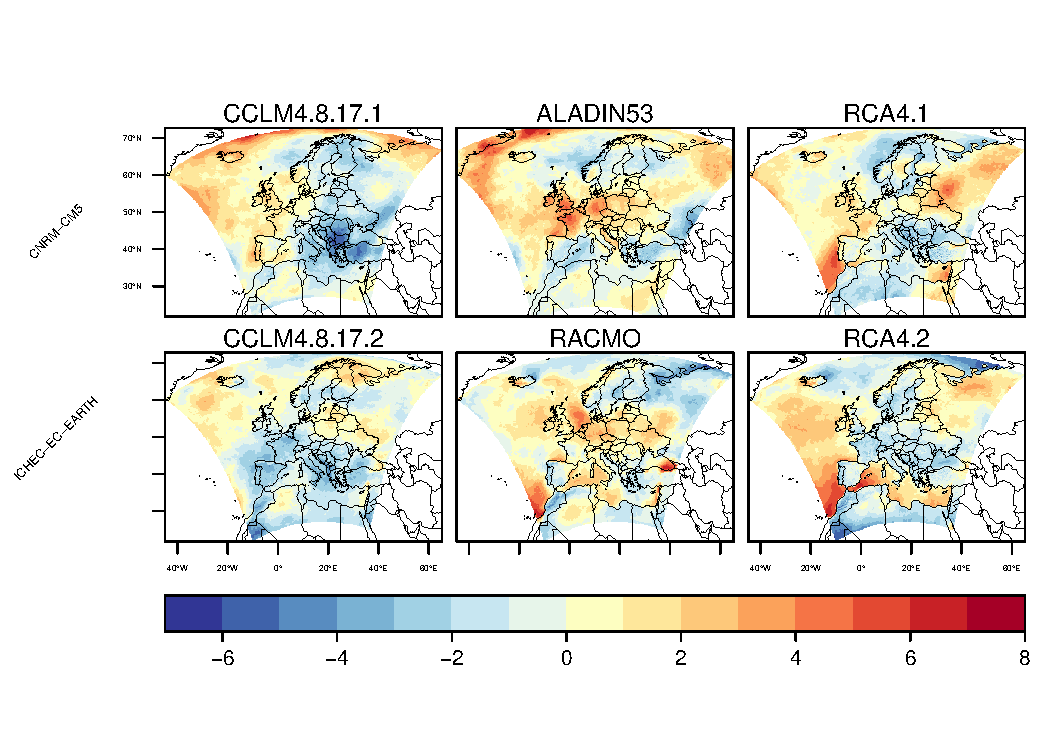
\includegraphics[width=1\textwidth]{figs/capitulo7/ANOMALIAS_JJA_CLT_2050-2021_r12.pdf}
\caption{}
\label{fig:anomalyCLT}
\end{figure}

\begin{figure}[h!]
\centering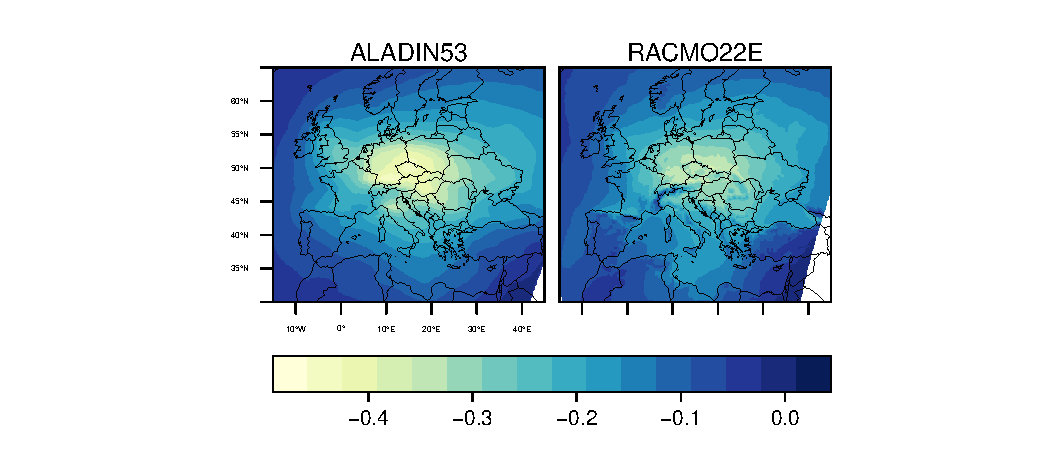
\includegraphics[width=1\textwidth]{figs/capitulo7/ANOMALIAS_JJA_AOD_2050-2021_r12.pdf}
\caption{}
\label{fig:anomalyAOD}
\end{figure}

\begin{table}
\caption{\label{tb:spatial correlations}Spatial correlation between SSR,CLT and AOD anomalies maps.}
\footnotesize
\begin{tabular*}{1\textwidth}{@{}llllllll}
\br
CMIP5 GCM & RCM & $\rho_{SSR,CLT}$  & $\rho_{SSR,AOD}$ & $\Delta{SSR}$ & $\Delta{CLT}$ & $\Delta{AOD}$ & $\Delta{PV_{annual}}$\\
\midrule
%  \mr 
CNRM-CM5&ALADIN5.3& -0.26 & -0.94 & 7.15 & 0.60 & -0.10 & 3.5$\%$\\
&CCLM4-8-17& -0.83 & - & -4.17 & -0.15 & - & -2.8$\%$\\
&RCA4& -0.71 & - & -3.55 & 0.21 & - & -2.6$\%$\\
\midrule
% \mr  
ICHEC-EC-EARTH&RACMO& -0.15 & -0.65 & 2.60 & 0.13 & -0.11 & -0.7$\%$\\
&CCLM4-8-17& -0.80 & - & -4.40 & -0.51 & - & -3.9$\%$\\
&RCA4& -0.59 & - & -3.44 & 0.09 & - & -3.6$\%$\\
%\midrule  
%HadGEM2-ES&RACMO& & & & & &\\
%&CCLM4-8-17& & & & & &\\
%&RCA4& & & & & &\\  
\bottomrule
%  \br
\end{tabular}\\
%$^{a}$UK spelling is required; $^{b}$MSC classification numbers are required; $^{c}$titles of articles are required in journal references; $^{d}$Harvard-style references must be used (see section \ref{except}); $^{e}$final page numbers of articles are required in journal references.
\end{table}
\normalsize

\subsection{Projected changes in PV production}

The photovoltaic yearly productivity, defined as the power output by the power capacity installed (it is consider a 1 kW system for each grid cell), is calculated for each pixel of land in the domain of EURO-CORDEX. Then, the averaged by country of the relative difference with respect to the reference period 1971-2000 is represented in next figure.

{\color{red} Anomalía para los modelos con aerosoles y los modelos sin aerosoles}

\begin{figure}[h!]
  \centering\begin{subfigure}{1\textwidth}
    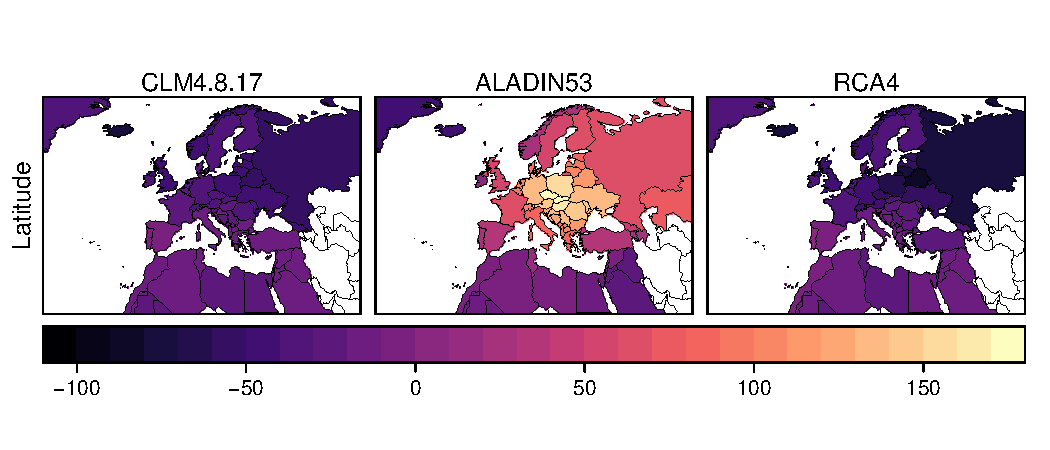
\includegraphics[width=1\textwidth]{figs/capitulo7/bycountry.pdf}
    \caption{a}
    \label{fig:diferenciaYm}
  \end{subfigure}
  %
  \centering\begin{subfigure}{1\textwidth}
    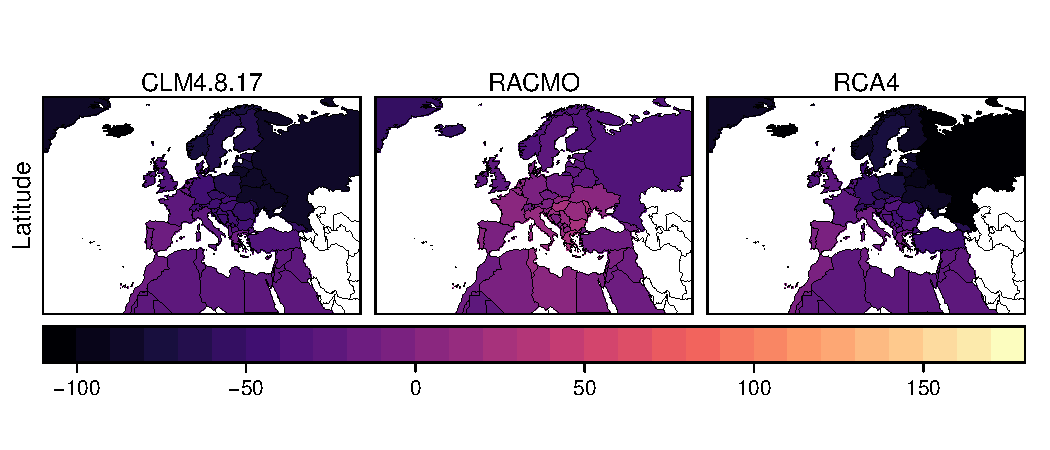
\includegraphics[width=1\textwidth]{figs/capitulo7/bycountry2.pdf}
    \caption{b}
    \label{fig}
  \end{subfigure}
  %
  \caption{}
\end{figure}

The geographical dependence of the PV anomaly is due to the spatial pattern of SSR anomaly, that is close related with the evolution of AOD in central Europe projected by ALADIN5.3 and RACMO22E. It is important to notice that for the ALADIN53 simulation including aerosols the sign in PV power output anomaly is positive and negative in the other cases. !!Besides, the RACMO anomaly is close to zero (although negative) whereas the rest of the simulation has the same magnitude order of the anomaly: ~ -2 to -4\%

%Uncertainties due to the different AOD datasets used in the two RCMs and in the radiative transfer code of the model difficults the robust answer about the change magnitude. Averaging the results for the non-aerosols simulations and aerosols simulation, we obtain the results in fugure.

\section{Discussion}

To determine the uncertainity in climate projections is one of the main issues in climate science because the information underlyng the simulations is difficult to comunicate. In order to isolate the uncertainity sources in a multi-model workit is necessary to design a sensitivity test for each of the models in the study. Up to now, there are not enough simulations from the EURO-CORDEX ensemble including evolving aerosols and for those that include them, there is not exist the same simulation excluding the aerosols forcing, in order to quantify its impact.

For that reason, this preliminary study, although it highlights very important issues, is the firs step in order to understand the role of aerosols in the RCM projections.

\section{Conclusion}

The study shows that regional climate models with evolving aerosols in the scenarios behaves different than those that has a fixed climatology. In the case of ALADIN53 the sign of the anomaly is reversed, agreeing with the positive signal in PV potential projected by GCMs.

It has been shown also that the anomaly of SSR is not directly linked with CLT anomaly in the case of the RCMs simulation that include evolving aerosols. The spatial correlation between SSR and CLT in this models is very low in comparison to the correlation between SSR and AOD anomaly.

The spatial pattern of the aerosols anomaly impact the future projections of PV differently in each country. The results show a general decresase for RCMs with no-evolving aerosols, more important in higher latitudes. However, for ALADIN53 and RACMO22E simulations the Central-Europe countries present a positive anomaly, which is relevant in terms of energy resource assessment.
% \end{document}
% \include{GeometriaSolar}

% \include{RadiacionSolar}

% \include{CelulaSolar}

% \include{AsociacionDispositivosFotovoltaicos}

% \include{SFCR}

% \include{SFER}

% \include{SFBombeo}

% \include{Seguridad}

% \include{EPBT}

% \nocite{Perpinan2009,Perpinan.Lorenzo.ea2009,Macagnan1993,Caamano.Laukamp.ea2008,Cleveland1993,Cleveland1994,Munoz2004,Tufte1990,Tufte2001}

\appendix

%\include{AnexoSimulacionBombeo}

% \include{EnlacesUtiles}

% \include{EjerciciosGeometriaRadiacion}

% \include{Ejercicios}

\backmatter

%%\bibliographystyle{flexbib}
%%\bibliography{../biblio}
\printbibliography

\end{document}
